\documentclass[12pt,twoside,a4paper]{article} 
\usepackage{fullpage}
\usepackage{graphicx}
\usepackage{natbib}
\usepackage{enumerate}
\usepackage{float}
\usepackage{url} % Better display of ~ tilde
\usepackage[leqno,fleqn]{amsmath}
\usepackage[polish,english]{babel} 
\usepackage[plmath,MeX]{polski} 
\usepackage[utf8]{inputenc}
\usepackage[font=footnotesize,format=plain,labelfont=bf,up,textfont=it,up]{caption}
\def\emptyline{\vspace{12pt}}
\pagenumbering{arabic}
\graphicspath{{./../}} % A path to the graphics directory
\numberwithin{equation}{subsection}
\numberwithin{figure}{subsection}
\selectlanguage{english} % We choose the autogenerated texts' language to be english
\addtolength{\voffset}{-1.0cm}
\linespread{1.7} %interline

\pagestyle{plain}
\title{Numerical evaluation of the Hilbert transform used to better understand 
and solve the Kramers-Kronig relations in nonlinear optics}
 \author{Krzysztof Parjaszewski}
 \date{}
\def\Xint#1{\mathchoice
{\XXint\displaystyle\textstyle{#1}}%
{\XXint\textstyle\scriptstyle{#1}}%
{\XXint\scriptstyle\scriptscriptstyle{#1}}%
{\XXint\scriptscriptstyle\scriptscriptstyle{#1}}%
\!\int}
\def\XXint#1#2#3{{\setbox0=\hbox{$#1{#2#3}{\int}$ }\vcenter{\hbox{$#2#3$ }}\kern-.6\wd0}}
\def\ddashint{\Xint=}
\def\dashint{\Xint-}
\newcommand{\ket}[1]{|#1\rangle}
\begin{document}
\maketitle
\section*{} \label{chap:preamble} 
\subsection*{Dedication} \label{chap:pre_dedication}


To my Family.


\section*{Abstract} \label{chap:abstract}
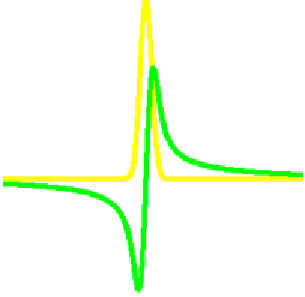
\includegraphics{img/title.png}
The motivation for this work comes from the real world problem stated by physicists and chemists emplyoing theoretical models to
describe the interaction between light and matter due to both low-level and intense light irradiation. The starting point is the
fundamental physical law - the causality principle - which states that the effect cannot precede the cause. This simple assumption
leads us to the Titchmarsh theorem about the Hilbert Transform - and together with advanced signal response-theory we can
investigate the properties of the medium response to the periodic input signal - both in time and frequency domain. Modifications
of the Hilbert Transform for the optical susceptibility $\chi (\omega )$ are known as the Kramers-Kronig relations - which are
defined for both real and imaginary part of susceptibility in the frequency-domain:

\begin{equation*}
  \Re (\chi (\omega ))=\frac {2}{\pi}\,\dashint_{ - \infty }^{\infty } \frac {\Omega \,\Im (\chi (\Omega ))}{\Omega ^{2} - \omega
  ^{2}} \,d\Omega 
\end{equation*}

\begin{equation*}
  \Im (\chi (\omega ))=\frac {2}{\pi}\,\omega \,\dashint_{ - \infty }^{\infty }\frac {\Re (\chi (\Omega ))}{\Omega ^{2} - \omega
  ^{2}}\, d\Omega 
\end{equation*}

where the integration uses the Cauchy principal value method. In this thesis we handle two problems. The first concerns numerical
problems with calculation of such a singular and improper integral. The second problem concerns the questions stated by physicists
- how to properly use these mathematical tools in a typical experiment and construction of a model useful in optical research. We
present comparison of several implementations of numerical calculations of the Hilbert transform:

\begin{itemize} \label{used_methods}
 \item Numerical trapezoidal rule mixed with the Simpson's rule and the
cubic interpolation
 \item Newton-Cotes qudrature of sixth degree
 \item Clenshaw-Curtis quadrature
 \item Hilbert transform based on fast Hartley transforms
 \item a method based on approximation with the orthonormal Hermite polynomials and Hermite functions
 \item a method based on approximation with the Fourier series.
\end{itemize}

We also test the out-of-the-box MATLAB-implemented routines:

\begin{itemize} \label{matlab_methods}
  \item quadgk()
  \item hilbert() - based on FFT
\end{itemize}
The given physical models for both linear and nonlinear optics are analysized and validated. We formulate hints for good practises
for scientists interested in the subject of optical experiments. Finally we make conclusions about the numerical stability,
advantages and disadvantages of the developed implementations in further research in nonlinear optics.

\emptyline

\subsection*{Keywords} \label{chap:abstract_keywords}
numerical analysis, nonlinear optics, Hilbert transform, Kramers-Kronig relations, optical dispersion relations

\subsection*{Promotors} \label{chap:abstract_promotors}

\subsubsection*{Nonlinear optics:}

\textbf{Professor Marek Samoć}

Institute of Physical and Theoretical Chemistry \\
Wroclaw University of Technology, PL-50-370 Wroclaw \\
Wybrzeze Wyspianskiego 27, Poland \\
+48-71-320-4466 | E-mail: Marek.Samoc@pwr.wroc.pl

\subsubsection*{Numerical analysis:}

\textbf{Paweł Keller PhD}

Group of Numerical Methods, Institute of Computer Science \\
University of Wroclaw, PL-50-383 Wroclaw \\
ul. Joliot-Curie 15, Poland \\
+48-71-375-7813 | E-mail: Pawel.Keller@ii.uni.wroc.pl

\subsection*{Author}  \label{chap:abstract_author}

\textbf{Krzysztof Parjaszewski}

Institute of Computer Science \\
University of Wrocław, PL-50-383 Wrocław \\
ul. Joliot-Curie 15, Poland \\
+48-660-070-043 | E-mail: Krzysztof.Parjaszewski@Gmail.Com

\subsection*{Reviewer}  \label{chap:abstract_reviewer}

\textbf{Professor Stanisław Lewanowicz}

Group of Numerical Methods, Institute of Computer Science \\
University of Wroclaw, PL-50-383 Wroclaw
ul. Joliot-Curie 15, Poland \\
+48-71-375-7813 | E-mail: Stanislaw.Lewanowicz@ii.uni.wroc.pl

\section{Introduction to nonlinear optics}  \label{chap:introducion}

\subsection{What is this thesis about?} \label{chap:introducion_what}

This thesis is a small step towards a better understanding the nature of light interaction with matter.

The main motivation and subject of this thesis is the application of numerical methods for better modelling and understanding the physical
models in nonlinear optics. The main experiment used during the work on this thesis has been conducted with the so-called Z-Scan
technique using a high-power femtosecond laser system consisting of a Quantronix Integra-C regenerative amplifier operating at
$800$nm and a Quantronix-Palitra-FS BIBO crystal-based optical parametric amplifier which allows one to obtain the output wavelength in
range of $\sim 450$nm up to $\sim 2000$nm. The laser pulses are of $\sim 130$ fs length and are delivered at $1$kHz repetition
rate. The experiments were performed at the Wroclaw University of Technology at the Institute of Physical and Theoretical
Chemistry. Numerical calculations were performed on a simple personal laptop within MATLAB and Maple environments.

The main numerical results concern the usage of the the Kramers-Kronig relations and the discussion about their application in
nonlinear optics. Firstly the simple linear Kramers-Kronig relation is derived and reviewed, then it is developed into a simple
nonlinear case. Next the perturbative approach and other modifications of the discussed model are reviewed. In each of these
examples, attention is paid to the numerical issues. The constructed numerical calculations are compared and discussed and further good practices for
physicists and chemists are formulated.

The subject of this thesis is not only an academic exercise - in last twenty years the global interest in photonics, and especially
application of light in modern devices for information transfer, storage and processing - including the construction of super-fast
all-optical computers - is steadily increasing. Recent years have seen much focus on the science and technology of photonics on
nano scale. In Poland - the nanophotonics research is being developed in several scientific centers among them in Wroclaw , which
would like to be one of the leading ones. To review both with Prof. MS and Dr PK.

\subsection{What is nonlinear optics?} \label{chap:introducion_nlo}

In mathematics a linear function f satisfies both of the following properties:

\begin{subequations}  \label{eq:linear_optics}
  \begin{equation}  \label{eq:nlo_additivity}
    \text{additivity:\,} \, \forall \, x, y : f(x+y) = f(x) + f(y)
  \end{equation}
  \begin{equation} \label{eq:nlo_homogeneity}
    \text{homogeneity:\,} \, \forall \, \alpha : f(\alpha\,x) = \alpha\,f(x)
  \end{equation}
\end{subequations}

Sometimes instead of talking of a function one taks about a ''system''. A nonlinear system is related to a function which does not
satisfy both additivity and homogenity simultaneosly. Another definition says that a nonlinear system does not follow the
superposition rule. The main area of interest for nonlinear optics is the behaviour of an optical wave in a nonlinear medium. In
the nonlinear case the superposition principle no longer holds, and therefore the response of a system/function depends nonlinearly
on the input signal. In practice the nonlinear behavior shows only at very high intensities of light, so the theory of nonlinear
optical effects is only applied to devices using high intensity light - such as modern lasers or optical fibers. Nonlinear optics
has strong links with physics, biology and chemistry but also mathematics and computer science, because modelling the
light behaviour is an open problem still being solved - which is schematically shown in figure \ref{fig:nonlinear_optics}:

\begin{figure} 
 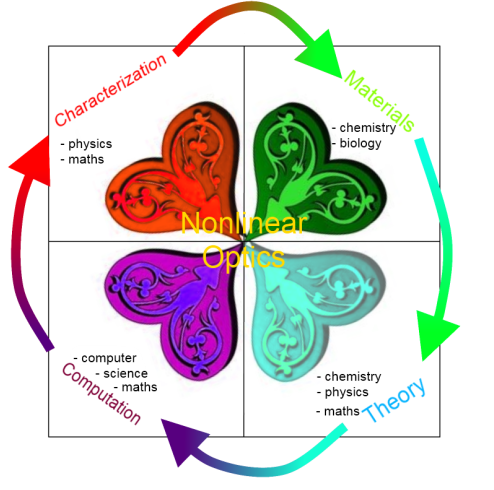
\includegraphics{img/nlo.png}
 \caption{Nonlinear optics derives from many foundamentary disciplines: biology, chemistry, math, physics and computer
 science \label{fig:nonlinear_optics}}
 
\end{figure}

A comprehensive, well prepared introduction to nonlinear optics can be found in the book ``\textit{Nonlinear Optics}'' written 
by Robert Boyd \cite{boyd_nlo}.

\subsection{What are the most important nonlinear optical properties and phenomena?} \label{chap:introducion_phenomena}

Experiments, which investigates the nonlinear nature of light interaction with matter may sometimes be similar to those in
classical optics, but they differ in the intensity of the radiation which is used. Modern lasers can routinely produce short pulses
of light with the duration of eg from $10$ femtoseconds up to several picoseconds and energy per pulse reaching mJ range thus a
single pulse from a laser can have power of giga-, tera- or even perawatts. Light intensities in the range of $\frac{G\,W}{cm^2}$
are commonly obtained even with lower powers by focusing of the laser beam. At these huge power of the light beam and the resulting
intensities - matter shows its nonlinear properties. Under the influence of the powerful and ultrafast lasers optical properties of
matter and the related phenomena such as refraction, diffraction, interference, dispersion, scattering of light etc. tend to
modify.

We define the following classification of the linear and nonlinear optical phenomena: \\
- linear phenomena \\
- second--order nonlinear phenomena \\ 
- third--order nonlinear phenomena \\
- nonlinear phenomena of higher orders
\begin{figure} 
  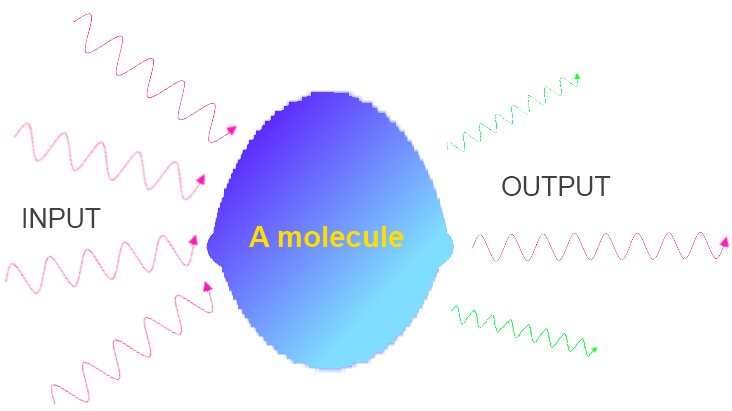
\includegraphics[width=150mm]{img/opt_phenom3.png}
  \caption{Schematic diagram of the nonlinear phenomenon -- the input beam(s') wavelength(s) may differ from the output signal(s).
  This happens only in case of the strong optical signals
  \label{fig:nonlinear_phenomenom}}
\end{figure}

The basis of such classification is the equation defined for the electric polarization by the classical electromagnetism. The
polarization density vector $\frac{C}{m^2}$ is approximated by the Taylor series: 

\begin{equation} \label{eq:polarization_taylor}
  \begin{split}
    \frac {{P_{i}}}{{\varepsilon_{0}}}=\frac {{P_{i}}(0)}{{\varepsilon_{0}}}
    + (\sum_{j=1}^{3}\,{\chi_{ij}}^{[1]}\,{E_{j}}) +
    + (\sum_{k=1}^{3}\,(\sum_{j=1}^{3}\,{\chi_{{ijk}}}^{[2]}\,{E_{j}}\,{E_{k}}))  \\
    + \left(  \! \sum_{l=1}^{3}\,(\sum_{k=1}^{3}\, (\sum_{j=1}^{3}\,{\chi_{ijkl}}^{[3]}\,{E_{j}}\,{E_{k}}\,{E_{l}}))
    \! \right) + \ldots
  \end{split}
\end{equation}

\begin{equation*}
  \mbox{for}\,i=1, \,2, \,3\,\mbox{with omission of}\,\frac {1}{n\mathrm{!}}\, \mbox{factors in the power expansion, }
\end{equation*}
where: 
\begin{equation*}
  \chi ^{[1]} : [\frac {m^{2}}{V^{2}}]
  \mbox{\,- the linear susceptibility tensor;}
\end{equation*}

\begin{equation*}
  \chi ^{[2]} : [\frac {m^{2}}{V^{2}}]
  \mbox{ - the second order nonlinear susceptibility tensor  }
\end{equation*}
- responsible for phenomena such as optical rectification (OR), second-harmonic generation (SHG), generation of sum and
differential frequencies (SFG and DFG) and Pockels electro-optic effect;
\begin{equation*}
  \chi ^{[3]} : [\frac {m^{2}}{V^{2}}]
  \mbox{ - the third order nonlinear susceptibility tensor  }
\end{equation*}

- responsible for phehonema such as intensity dependent refractive index (IDRI), third harmonic generation (THG), stimulated
brillouin scattering (SBS), stimulated Raman scattering (SRS), degenerate four waves mixing (DFWM)
and nonlinear absorption \cite{samoc_nlo_opt_mat}. 

The intensity dependent refractive index (IDRI) can be described by the equation:

\begin{equation} \label{eq:refr_idri}
  n={n_{0}} + [{n_{2}}]\,\langle E^{2}\rangle \mbox{,}
\end{equation}

where: 

\begin{equation*}
  {n_{0}} \mbox{ - the weak-field refractive index;}
\end{equation*}
\begin{equation*}
  [{n_{2}}] \mbox{ - the nonlinear index of refraction;}
\end{equation*}
\begin{equation*}
  \langle E^{2}\rangle \mbox{ - means the time averaged $E^2$.}
\end{equation*}

$[n_2]$ is a new optical constant which describes the change of the refractive index in the relation to the strength of
the optical signal. Alternatively, the nonlinear refractive index may be related to the light intensity \textit{I} since \textit{I} is
proportional to the square of the electric field amplitude.

The intensity-dependent change in the refractive index is sometimes called the optical Kerr effect. It is a similar effect to
the Kerr electro-optic effect, which is a modification of the refraction index under the influence of the strong electric field
applied to the medium. In the optical case the change of refraction index comes only from the influence of very intense light beam,
typically from a laser system. The theory beneath this effect has its roots in a quantum mechanics effects (e.g. the dynamic
Burstein-Moss effect) and the more advanced quantum chemical description of the $[n_2]$ can be found in the most recent
nanophotonics literature (e.g. chapter $5$ in \cite{christodoulides_nonlinear}).

Several effects come as the result from the indensity dependent refractive index:
\begin{itemize}  
  \item self-focusing of light - focusing the light beam within the nonlinear medium;
  \item two beam coupling - is the energy transfer between two light beams interaction within the nonlinear medium. This effect
  requires a special type of ``nonlocal" refractive index changes typically found in so-called photorefractive phenomena;
  \item optical phase conjugation - can be used for reversing the typical abberation effects;
  \item all-optical switching - is the very interesting effect which allows to control the flow of one beam of light by another. In
  other words it is a control of light by light.
\end{itemize}

The nonlinear absorption may concerns the absorption of energy from two or more photons influencing matter in the very 
same moment of time or the absorption of light under the heavy light intensity. Both linear and nonlinear absorption 
process has the property of spatial selectivity, which means that the with different angle of light beam incidenting on 
matter we get different absorption coefficients - which is related to the tensor nature of the optical susceptibility. 
Also the polarization geometry of the light beam plays important role here \cite{boyd_chirality}.

\textit{Description of determination the nonlinear optical properties and describing the NLO phenomena in several sentenses}

\subsection{Why is nonlinear optics so important?} \label{chap:introducion_rank}

Nonlinear optics is the widely investigated area in nanophotonics, because a material with a high nonlinear refractive 
index will be a key to to build an all-optical-transistor and such device should work as an all-optical logic gate. 
That will lead us to create the ultra-fast optical devices, for instance the photonic computer - where instead of electrons, 
photons will be used to perform computations with a very high speed. Some scientists suggest that the taming of 
all-optical-switching phenomenom is the Holy Grail of modern photonics \cite{samoc_nlo_opt_mat}.

On the other hand - the nonlinear absorption, which is strongly related to the nonlinear refraction index - is an important obstacle
to build such a fast all-optical-device. Despite ot that, nonlinear absorption still may be very useful in nanofabrication, biophotonics,
microscopy, information storage and other technologies using short laser pulses \cite{samoc_nlo_absorption}. 

The interest in nonlinear optics comes from both the basic research and industry. The basic research and fundamental questions in material
research concerns the nature of light, optical properties of molecules, the strength and properties of chemical bonds and theory to
determine both linear and nonlinear optical properties insead of performing myriads of experiments. The industrial research interests
in nonlinear optics are mostly focused in the area of developing new optical devices (detectors, engines, logic gates, fibers, lasers and
more) and the usage of intensive light beams for various types of screening and determing the 3D information about the geometrical of
the investigated material.

\textit{Description of the most expected results of understanding the nonlinear optics.}

\subsection{Why should we use Kramers Kronig relations here?} \label{chap:introducion_kk}

Kramers Kronig relations are the fundamental tools in the exploration of the material optical properties and together with other classical
physics and quantum mechanics predictions can be used to construct and validate theoretical models. They are originated from the most basic
but also very important law in physics - the causality principle. From the philosophical perspective it states that each effect must be
preceded by a cause. In computer science this principle is somehow paraphrased in a discussion of formal deterministic and
nondeterministic automatas. We believe that only deterministic automatas really exist. 


\begin{subequations}  \label{eq:kk_basis}
 \begin{equation}  \label{eq:kk_basis_ift}
   \Psi (t) = \mathbf{IFT}(\Psi (\omega ))
  \end{equation}
  \begin{equation} \label{eq:kk_basis_casuality}
    \forall t < 0 : \Psi (t) = 0
  \end{equation}
\end{subequations}

The causability principle looks obvious, but in the field of nonlinear optics - combined together with the application of the inverse Fourier
transform of any nonlinear quantity spectrum: $\Psi (\omega )$ , $\textbf{R} \ni \omega$ - it states that the time-domain signal 
$\Psi (t)$ calculated with \ref{eq:kk_basis_ift} from frequency-domain must equal zero for any negative time argument. This statement 
can be used in validation of any spectrum $\Psi (\omega )$ , $\textbf{R} \ni \omega$ - what is important when we only measure the 
physical quantity in aspecific range $\exists a,\,b : a < \omega \wedge \omega < b$. We simply cannot measure the whole real spectrum 
$\textbf{R} \ni \omega $ and in this case we need to perform the validation of approximated or assumed spectrum $\Psi (\omega )$.

Kramers Kronig relations - which will be derived in the following chapter - connects the real and imaginary part of the Fourier
transform of valid response signal. It is said that one can derive the real part of the determined spectrum $\Psi (\omega )$. What is 
even more important - this relation is bidirectional - so with the Kramers Kronig relations one can derive the imaginary part from real. 
This hypothesis has been formulated in 1948 by Edward Charles Titchmarsh - with the tacit assumption, that both $\Psi (t)$ and 
$\Psi (\omega )$ are the square-integrable functions and more - the $\Psi (\omega )$ holomorphic in the upper-plane. This simple theorem 
- is widely investigated area in both the nonlinear and linear optics - to connect the refraction index togheter with absorption coefficient, 
which are th real and imaginary parts of the optical susceptibility respectively.

\textit{Just few words about the hopes of using K-K relations also in nonlinear optics.}

\subsubsection*{Notes}

1. ''Znajomość pełnej funkcji dielektrycznej $\varepsilon (\omega )={\varepsilon_{1}}(\omega ) + i\,{\varepsilon_{2}}(\omega )$
 daje nam klasycznie pełny opis zjawisk towarzyszących rozchodzeniu się fali elektromagnetycznej w materii.''
2. Teorię fitowania lorentzianów opisuje regresja nieliniowa.
3. Dopisać referencje do fragmentu dotyczącego kwantowo-chemicznego opisu n2

\textit{Some notes in both polish and english.}

\section{Problem definition (understanding)} \label{chap:problem}

\subsection{Linear model} \label{chap:problem_lin}

Basically in the linear optical model we assume, that the response of a medium depends linearly on the input. The similar presumption is
made in many fields of physics - for instance in magnetostatics we linearly connect the current density \textbf{J} with the electric
field \textbf{E} vector multiplied by a conductivity parameter $\sigma $ - which is called the Kirchhoff's reformulation of the Ohm's Law:

\begin{equation} \label{eq:ohms_law}
  \textbf{J} = \sigma \textbf{E}
\end{equation}

As it will be shown later, such relations hold for sufficiently small intensities - but the definition of 'sufficiently small' will not be
further specified. In the time-domain it is stated that an external sinusoidal electromagnetic radiation of a light beam - \textbf{the
input} - is defined by a field vector:

\begin{equation} \label{eq:electromagnetic_radiation}
  \textbf{E} (\textbf{r}, t) =  \frac{1}{r} {E_{0}} cos(\textbf{k r} - \omega t + \phi) \mbox{,}
\end{equation}

where:
$\textit{\textbf{k}}$ - wave vector (radians per meter) \\
$\textit{\textbf{r}}$ - position vector (meters) \\
$t$ - time (seconds) \\
$\omega $ - angular frequency (radians per second) \\
$\phi $ - phase shift (radians)

\textbf{The output} - reponse in the form of polarization vector can be described using the linear response theory - which is the
simplification of the Volterra series that takes only the leading order term can be described as the following convolution:

\begin{equation} \label{eq:polarization_volterra}
  {P_{1, \,i}} (\textbf{r}, t) = {\varepsilon_{0}}\, \left(  \! \sum_{j=1}^{3}\,\int_{ -
  \infty }^{\infty }\int {G_{1, \,i, \,j}}(p - r, \,s - t)\,{E_{1,\,j}}(p, \,s)\,dp\,ds \!  \right)
\end{equation}
with the inner integral made through the Euclidean space $R^{3}$ \cite{thesis_novak},\\
where: \\
${1}$ -- the '1' index states for linear property of any investigated value \\
${P_{1, \,i}}$ -- 3x1 real linear polarization tensor (vector) in a spacetime-domain, $i$ stays for chosen spatial coordinate (x, y or z)
$[\frac {C}{m^{2}}]$ \\
${G_{1, \,i, \,j}}$ - 3x3 real susceptibility tensor (matrix) defined by a linear Green function in a spacetime-domain \cite{fakiszscan} \\
${E_{1, \,j}}$ - 3x1 real electric field tensor (vector) in a spacetime-domain $[\frac {V}{m}]$ \\
${\varepsilon_{0}}$ - electric permittivity of free space $8.854187817620 x\,10^{( - 12)}$ \\
$\frac {C}{V\,m}$  -  position vector (meters)  \\
$t$ - time (seconds)

Even such linear equation is only the simplification, because we do not assume the local field corrections \cite{chui_lf_correction}. It seems to be an
reasonable assumption as long as we emphasize the macroscopic character of polarization. Only in case of constructing very small
devices or synthesizing small particles - we shall take the local field interaction into account. Investigation of the properties of the
susceptibility tensor both in time-domain and frequency-domain will be the main part of considerations in this thesis - it is also widely
discussed topic in the literature \cite{boyd_nlo, prasad_intro_nlo, Levenson_dispersion, trager_springer, bloembergen_nonlinear}.

The Fourier transform allows us to change the polarization equation \ref{eq:polarization_volterra} from time domain to frequencydomain:

\begin{equation} \label{eq:polarization_frequency}
   \Phi \{ \textbf{F} P_{1, \, i} ( \textbf{r}, t) \} = P_{1, \, i} (\textbf{k}, \omega )
\end{equation}

where: \\
$\Phi $ - Fourier transform operation in $3$D space domain \\
\textbf{F} - Fourier transform operation in time domain \\
${P_{1, \,i}} (\textbf{k},\omega )$ - $3$x$1$ complex linear polarization tensor (vector) in a wave-frequency domain,
                                        $i$ stays for chosen spatial coordinate (x, y or z) $[\frac {C}{m^{2}}]$ \\
$\textbf{k}$ - $3$x$1$ wave tensor (vector) of the electromagnetic field $[\frac {1}{m}]$ \\
$\omega $ - angular frequency of the electromagnetic field $[\frac {rad}{s}]$


Due the convolution theorem \cite{katznelson_introduction} the Fourier transform applied to the convolution of two given functions equals
the simple multiplication of two Fourier transforms:
\begin{equation} \label{eq:convolution_theorem}
  \Phi \textbf{\{F}[ {\varepsilon_{0}}\, \left(  \! \sum_{j=1}^{3}\,\int_{ - \infty }^{\infty }
    \int {G_{1, \,i, \,j}}(p - r, \,s - t)\,{E_{1, \,j}}(p, \,s)\,dp\,ds \!  \right) =
    {\varepsilon_{0}}\,(\sum_{j=1}^{3}\,{\chi_{1, \,i, \,j}}(k, \,\omega )\,{E_{1, \,j}}(k, \,\omega )),
\end{equation}

where: 

\begin{tabular}{r l}
  $\Phi $ & - Fourier transform operation in $3$D space domain \\
  $\textbf{F}$ & - Fourier transform operation in time domain \\
  ${\chi_{1, \,i, \,j}} (\textbf{k},\omega) $ & - 3x3 complex susceptibility tensor in a wave-frequency domain
  \cite{fakiszscan} \\ ${E_{1, \,j}} (\textbf{k}, \omega) $ & - 3x1 complex electric field tensor in a wave-frequency
  domain $[\frac {V}{m}]$ \\
\end{tabular}


\emptyline


From \ref{eq:polarization_frequency} and \ref{eq:convolution_theorem} we get:

\begin{equation} \label{eq:final_linpolarization}
  {P_{1, \,i}}  (\textbf{k}, \omega) = {\varepsilon_{0}}\,(\sum_{j=1}^{3}\,{\chi_{1, \,i, \,j}}(k,\,\omega )\,{E_{1, \,j}}(k, \,\omega ))
\end{equation}

which seems to be a simpler equation - so from now we will use the wave-frequency domain. We will no be getting further into the physical
details of the optical susceptibility theory. For our interests it is worth stressing, that the ${G_{1, \,i, \,j}}$  - 3x3 real susceptibility
tensor (matrix) defined by a linear Green function in a space-time domain follows the following rules:

\begin{subequations}  \label{eq:green_properties}
 \begin{equation}  \label{eq:green_causality} (\textbf{r}, t) = 0
   \mbox{the causality principle: } {G_{1, \,i, \,j}}
  \end{equation}
  \begin{equation} \label{eq:green_energy}
    \mbox{the convservation of energy law: }  \forall \textbf{r} : \int_{ - \infty }^{\infty }{G_{1, \,i, \,j}}(r, \,t)\,dt <  \infty
  \end{equation}
\end{subequations}

The Fourier transform is defined for integrable functions and after \cite{muhoray_course,lucarini_kramers} we can assume the asymptotic
behaviour of the susceptibility tensor in wave-frequency domain:
\begin{equation} \label{eq:susceptibility_wavefrequency}
  F[ G_{1, \,i, \,j} (\textbf{r} ,t) ] = \chi_{1, \,i, \,j} (\textbf{k}, \omega ) = - \frac {C}{\omega ^{2}} + o(\omega ^{( - 2)}),
\end{equation}
where: 

\begin{tabular}{r l}
  $C$ & - is a material specific constant, which does not depend on $\omega $ \\
  $o(\omega ^{( - 2)})$ & - indicates a term with asymptotic descrease stricly faster then $\frac {1}{\omega ^{2}}$ \\
\end{tabular}


From the physical point of view such a vanishment is true - because for an input oscillation with a frequency much higher than any
resonant frequency - the system will have not enough time to responde before the input signal has switched it direction, so for large
$\omega $ the susceptibility ${\chi_{1, \,i, \,j}}(\textbf{k},\omega )$ vanishes.


Also from the conservation of energy law we assume, that:
\begin{equation} \label{eq:susceptibility_conservation}
  \exists \textbf{K} < \infty, \forall \textbf{d}, \omega : chi_{1, \,i, \,j}(\textbf{k}, \omega) < \textbf{K}
\end{equation}


Together with the knowledge of asymptotic behaviour from \ref{eq:susceptibility_wavefrequency} we will concluded, that the susceptibility
tensor is also square integrable:

\begin{equation} \label{eq:susceptibility_sqrintegrable}
  \chi_{1, \,i, \,j}(k, \,\omega ) \,\in \,L \Rightarrow \chi_{1, \,i, \,j} (k, \,\omega )\,\in\,L^{2}
\end{equation}


\textit{Description of linear model of dispersion}

\subsection{Derivation of the Kramers-Kronig for linear model} \label{chap:problem_dlin}

Before we will focus on the final form of the Kramers-Kronig relations - we shall stress that they are the reformulation of the Titchmarsh theorem
in area of Fourier analysis. This theorem relates real and imaginary parts of the functions from the upper half-plane of the Hardy space:
$H^{p}$ with the Hilbert transform of a function from $L^{p}$.

\subsubsection*{Titchmarsh theorem:}

\textbf{Let:}
\begin{subequations}  \label{eq:titchmarsh_theorem}
 \begin{equation}  \label{eq:titchmarsh_assumption}
   a(t)\,\ \in \,L^{2}(\mathbf{R}) \wedge \forall t < 0 : a(t) = 0
  \end{equation}
  \begin{equation} \label{eq:titchmarsh_thesis}
    \mbox{Then: }  b{\omega} = F[a(t)] \wedge b \in H^2(\textbf{U}),
  \end{equation}
\end{subequations}

where:

\begin{tabular} {r l}
  $H^{2}$ & - Hardy space of the holomorphic functions with a norm: \\
  \, & $\sup_{y > 0} [\int  \left|  \! \,\mathrm{f}(x + i\,y)\, \!  \right| ^{2}\,dx] ^{(\frac {1}{2})} < \infty$ \\
  $\mathbf{U}$ & - the upper-half complex plane, \\
  $F$ & - Fourier transform functional \\
\end{tabular} 

\begin{subequations}  \label{eq:titchmarsh_relations}
  \begin{equation}  \label{eq:titchmarsh_real}
    \Re (\mathrm{b}(\omega )) =  \frac{1}{\pi}\,\int_{ -\infty }^{\infty }
    \frac {\Im (\mathrm{b}(\Omega ))}{\Omega - \omega }\,d\Omega 
  \end{equation}
  \begin{equation} \label{eq:titchmarsh_imag}
    \Im (\mathrm{b}(\omega )) = -\frac{1}{\pi}\,\int_{ -\infty}^{\infty }
    \frac {\Re (\mathrm{b}(\Omega ))}{\Omega - \omega }\,d\Omega,
  \end{equation}
\end{subequations}

where:

\begin{tabular} {r l}
  $\Re (\mathrm{b}(\omega ))$ & - real part of $b(\omega)$ \\
  $\Im (\mathrm{b}(\omega ))$ & - imaginary part of $b(\omega)$ \\
\end{tabular}


To omit the singularity - the integral values is calculated using the Cauchy principal value.

What's more - the theorem states that \ref{eq:titchmarsh_assumption}, \ref{eq:titchmarsh_thesis} and \ref{eq:titchmarsh_relations}
are mathematically equivalent. Proof with an exhausting review of both the Fourier and Hilbert transforms has been described by Edward
Charles Titchmarsh in \cite{titchmarsh_introduction} - the theory is described through all book
chapters, but the theorem and its proof has been stated in chapter $5$ about the conjugated integrals also called the Hilbert transforms.

We have nearly state the Kramers-Kronig relations. If we take a closer look into equation \ref{eq:susceptibility_wavefrequency} we will see that:

\begin{subequations} \label{eq:susceptibility_properties}
  \begin{multline}   \label{eq:sproperties_longer}
     {\chi_{1, \,i, \,j}} (k, \, - \omega ) = F[{G_{1, \,i, \,j}}(\textbf{r} ,-t)] = \int_{0}^{\infty }\int_{0}^{\infty }
     {G_{1, \,i, \,j}}(\mathit{\xi}, \,\tau )\,e^{(i\,\omega \,\tau )}\,d\tau\,e^{( - i\,k\,\xi )}\,d\xi
     \\ = [{\chi_{1, \,i, \,j}} (k, \,\omega )] = [{\chi_{1, \,i, \,j}} (k, \,\omega )]
  \end{multline}
  \begin{equation}   \label{eq:sproperties_shorter}
    {\chi_{1, \,i, \,j}} (k, \, - \omega ) = [{\chi_{1, \,i, \,j}}(k, \,\omega )]
  \end{equation}
\end{subequations}


where: 

\begin{tabular} {r l}
  * & - the symbol denoting the complex conjugate. \\
\end{tabular}


With such assumption we deduce that:
\begin{subequations} \label{eq:susceptibility_deduces}
  \begin{equation}   \label{eq:sdeduces_Re}
     Re \{ {\chi_{1, \,i, \,j}} (k, \,\omega ) \} =  Re \{ {\chi_{1, \,i, \,j}}(  k, \, -\omega ) \}
  \end{equation}
  \begin{equation}   \label{eq:sdeduces_Im}
     Im \{ {\chi_{1, \,i, \,j}} (k, \,\omega ) \} = -Im \{ {\chi_{1, \,i, \,j}}( -k, \,  \omega ) \}
  \end{equation}
\end{subequations}
Now the previous equation \ref{eq:susceptibility_properties} can be written in a new form:
\begin{subequations} \label{eq:susceptibility_new}
  \begin{equation}   \label{eq:snew_Re}
     \Re ({\chi_{1, \,i, \,j}}(k, \,\omega ))=\frac {2\,\int_{0}^{\infty }
     \frac {\Omega \,\Im ({\chi_{1, \,i, \,j}}(k, \,\Omega ))}{\Omega ^{2} - \omega ^{2}}\,d\Omega }{\pi }
  \end{equation}
  \begin{equation}   \label{eq:snew_Im}
     \Im ({\chi_{1, \,i, \,j}}(k, \,\omega ))=( - \frac {2\,\omega }{\pi })\,\int_{0}^{\infty }
     \frac {\Re ({\chi_{1, \,i, \,j}}(k, \,\Omega ))}{\Omega ^{2} - \omega ^{2}}\,d\Omega
  \end{equation}
\end{subequations}
We will further forget about the \ref{eq:susceptibility_properties} assumption, because firstly there is no difference in the computation
complexity between \ref{eq:susceptibility_properties} and \ref{eq:susceptibility_new}. What is more - this assumption has sense
only from the mathematical point of view, we supose that it should be dismissed in any further calculations as an ''artefact'' - because in
all experimental fitting we supose that the absorption peak has Gaussian or Lorentzian distribution - which is a not an odd nor an
even function and we would have artificially assume that should tends to zero near the zero frequency - which not always must be true.

For the first look the relations  \ref{eq:susceptibility_new} may look not so impressive, but we must have in our mind that the real and imaginary
part of susceptibility describes two completely different optical phenomena - the refraction of light and the absorption of light. If we
like to measure them - in most cases - we will need to perform two different experiments. Kramers-Kronig relations allows us to imply -
that for now we only need to properly measure one of this two values - and the other can be calculated on the basis of its results. This is
of course the half-true. Taking into consideration many in uncertainities and experimental errors it is also an good idea to
measure both values - and then check if the theoretical model in which we describe the optical properties of investigated material - is valid and therefore we can proof its self-consistency.

\textit{Derivation of the Kramers-Kronig relation for linear optics.}

\subsection{Simple nonlinear model} \label{chap:problem_nlo}

It is true that our knowledge about the linear interaction between the light and matter has been investigated in recent several decades quite
well. We shall even say that this scientific area has been described almost completely. The really interesting and important from the
scientific point of view is the area of nonlinear optics - when more than one light wave interact with matter in a definite, extremely
short period of time with a length of femto- or even attoseconds. When two or more photons 'shoot' an atom or a molecule - we may observe
many new kinds of physical phenomena. From the quantum physics point of view - each photon transports some amount of energy depending on
its frequency. More energy in a short time period - means a higher chance for the molecule to modify its spatial structure, electron
energy or some other property.

We shortly describe the time-resolved processes which allow to determine the origin of two important nonlinear processes: the pump-and-probe and
the frequency mixing process.

\subsubsection*{Pump-and-probe process}

In a typical pump-and-probe process we observe two laser beams. One of them is a strong signal - called the 'pump' - the second signal - the
'probe' - is much less intensive. We try to synchronize this two laser beams in a following way - firstly a pump signal hits the sample with
its strong intensity - causing modifications in the sample properties. Shortly after that - within a time period
$\Delta \, t$ - a low-intesive probe signal hits the modified sample and runs through the detector. In a typical experiment the
$\Delta \, t$ time period should be adjustable. There are usually much more detectors, but we are mostly interested in the polarization amplitude
of the probe response signal. An important assumption for both pump and probe beams is for them to be in the same polarization. The
schematic diagram of a pump-and-probe process has been described on the \ref{fig:pump_and_probe}.

\begin{figure} 
  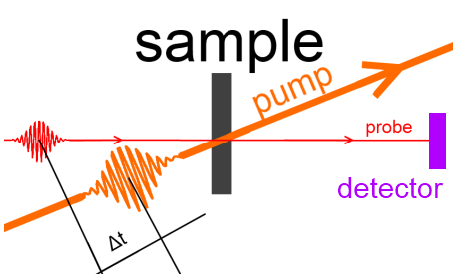
\includegraphics{img/pnp.png}
  \caption{The pump-and-probe process\label{fig:pump_and_probe}}
\end{figure}


The key assumption in the pump-and-probe process is that separated and independent probe signal cannot saturate the response of atomic system
alone \cite{boyd_nlo}. The probe signal shall be that weak - it will not cause any more nonlinear effects in the investigated medium. It is
important that investigated molecule has for both the pump and the probe signal two different relaxation times: ${T_{1}}$  and ${T_{2}}$
respectively. A complicated model is defined by H. N. Yum et al. \cite{yum_pump} for the nonlinear susceptibility in case of pump-probe process:

\begin{multline}   \label{eq:pump_equation}
     {\chi_{pp}}(\delta ) = \frac {G\,n^{0}\,{\gamma_{ba}}}{\Delta  + \delta  + i\,\eta } \cdot \\
     [1 - \frac {{\Omega_{1}}^{2}\,(\Delta  - \delta  + i\,\eta )\,(\delta  + 2\,i\,\eta )}{(\Delta  - i\,\eta )\,((\delta  + i\,
     teta)\,(\Delta  + \delta  + i\,\eta )\,(\delta  - \Delta  + i\,\eta ) - {\Omega_{1}}^{2}\,(\delta  + i\,\eta ))\,2}],
\end{multline}

where: ${\Omega_{1}} = \Omega_{1} ({T_{1}}), G = G({T_{1}}), n^{0} = n^{0}({T_{1}}), \gamma_{ba} = \gamma_{{ba}}({T_{1}}), \eta =
\eta ({T_{1}})$ and 

\begin{tabular} {r l}
  $\delta $ & - probe frequency \\
  $\Delta $ & - pump prequency \\
\end{tabular}



where particular parameters depend on the complicated derivation with an usage of quantum-mechanics and classical-mechanics approach. Here
the important thing to concider is that the susceptibility of the probe depends on the relaxation time of pump signal - which in other
words means that:

\begin{equation} \label{pump_depend}
  \chi_{pp} = \chi_{pp}(\delta, T_{1}) \mbox{ and } T_{1} = T_{1}(\Delta \, t)
\end{equation}

In sense of the response theory this observation leads us to the conclusion, that the suscebility of the nonlinear process depends not
only on the input signal frequency (energy) - but also on the time delay between the moments, when two or more photons shots the
molecule. The literature we have found is in lack of advanced model - so here we are talking about the cutting edge problem in nonlinear
optics and the constructing of the valid model for the pump-and-probe process - so the Kramers-Kronig relations should be applied here. We
also deduce from the response theory, that the output signal in the pump-and-probe process does not shows instantly, but after the last
photon shots the investigated molecule - so we have some type of pause - which observation should expand the linear response theory.

In \cite{christodoulides_nonlinear} we can found results that proofs that the probe signal absorbance depends not only on the pump signal
properties, but also on the delay time between the pump and probe - see \ref{fig:pnp_absorption}.

\begin{figure} 
  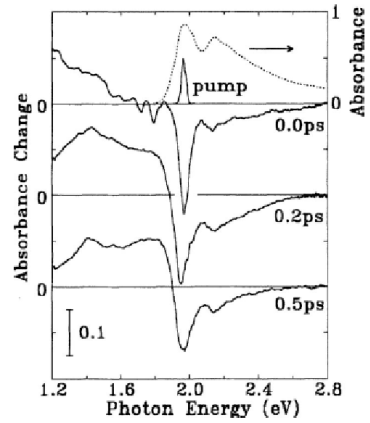
\includegraphics{img/pnp_abs.png}
  \caption{The pump-and-probe absorption change dure to time delay between the pump and probe signal.
  Figure taken from \cite{christodoulides_nonlinear} \label{fig:pnp_absorption} }
\end{figure}

The more interesting results come when we assume, that susceptibility is a complex function of two parameters, both the pump and
probe signal frequency:

\begin{equation} \label{eq:pnp_2args}
  \chi_{pp} = \chi_{pp}(\delta , \,\Delta )
\end{equation}

Therefore we obtain such an 3-Dimensial plots:

\begin{figure} \label{fig:pnp_2d}
  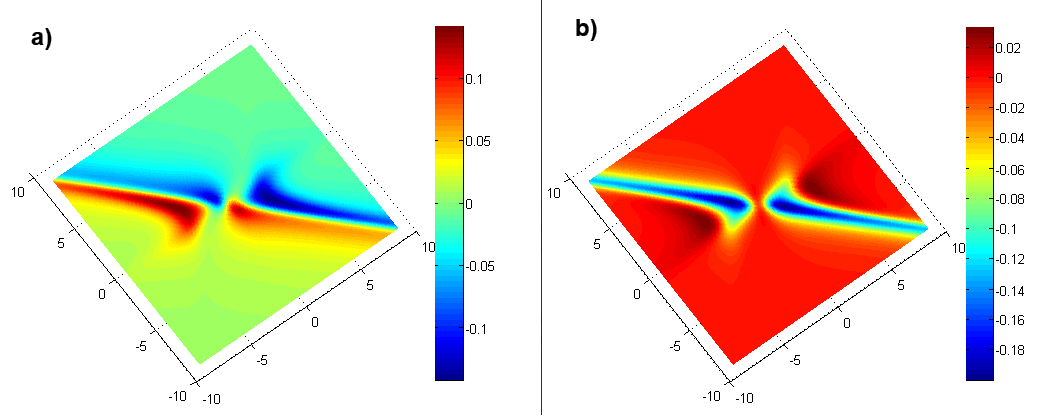
\includegraphics[width=150mm]{img/pnp_2d.png}
  \caption{2-Dimensial plots of both a) real and b) imaginary parts of nonlinear susceptibility threated as a biargumental
  function, where the color means the function value}
\end{figure}

\begin{figure} \label{fig:pnp_3d}
  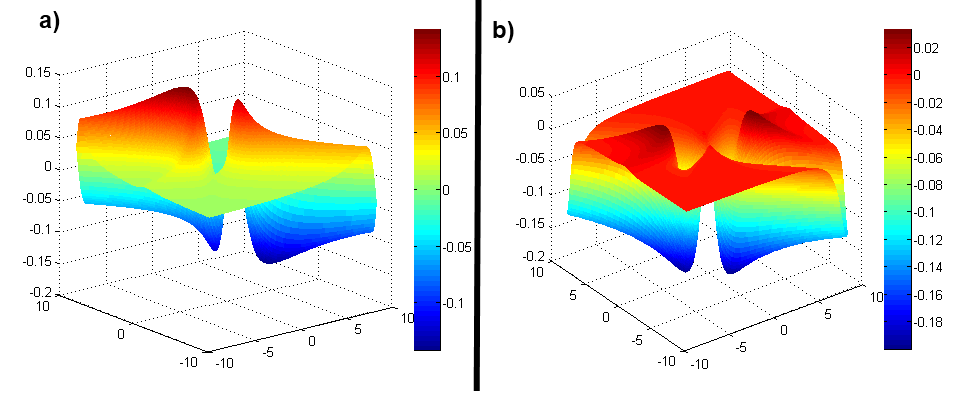
\includegraphics[width=150mm]{img/pnp_3d.png}
  \caption{3-Dimensial plots of both a) real and b) imaginary parts of nonlinear susceptibility threated as a biargumental
  function, where the color means the function value}
\end{figure}

\subsubsection*{Frequency Mixing Process}

The frequency mixing is a general class of processes when we have two or more input photons with their frequencies:
${\omega_{input, \,1}}, \,{\omega_{input, \,2}}, \,{\omega_{input, \,3}}, \ldots $ and we receive one or more output photons with
their frequencies: ${\omega_{output, \,1}}, \,{\omega_{output,\,2}}, \,{\omega_{output, \,3}}, \ldots $. In chapter 6.6 of Boyd
\cite{boyd_nlo} we can find the description of process in which we observe the strong singal 'pump' with frequency $\omega$ andthe
weak signal 'probe' with the frequency $\omega  - \delta $ nearly copropragating, as has been shown on the figure \ref{fig:fmix_sch}.

\begin{figure} 
  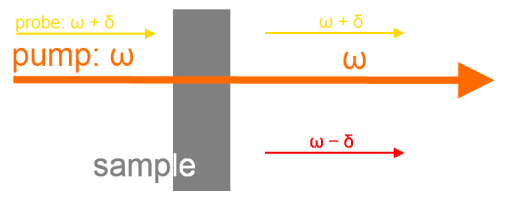
\includegraphics{img/fmix_sch.png}
  \caption{The pump-and-probe frequency mixing process from chapter 6.6 Boyd \cite{boyd_nlo} \label{fig:fmix_sch}}
\end{figure}

For such process a model for the linear susceptibilities has defined by Boyd for both $\omega  + \delta $ and $\omega  - \delta $
frequencies:

\begin{subequations} \label{eq:fmix_eff1}
  \begin{equation}   \label{eq:feff1_plus}
    \chi_{eff, \,1}(\omega  + \delta ) =
     \frac {N\, \left|  \! \,{\mu_{ba}}^{2}\, \!  \right| \,{w_{0}}\,(\delta  + \frac {i}{{T_{1}}})\, \left(  \! \delta  -
     \Delta  + \frac {i}{{T_{2}}} - \frac {\Omega ^{2}\,\delta }{2\,(\Delta  - \frac {i}{{T_{2}}})} \!  \right) }{{\varepsilon_{0}}\,
     h\,\mathrm{D}(\delta )}
  \end{equation}
  \begin{equation}   \label{eq:feff1_minus}
    \chi_{eff, \,1}(\omega  - \delta ) =
     \frac {N\, \left|  \! \,{\mu_{ba}}^{2}\, \!  \right| \,{w_{0}}\,( - \delta  + \frac {i}{{T_{1}}})\, \left(  \!  -
     \delta  - \Delta  + \frac {i}{{T_{2}}} + \frac {\Omega ^{2}\,\delta }{2\,(\Delta  - \frac {i}{{T_{2}}})} \!  \right) }{{
     \varepsilon_{0}}\,h\,\mathrm{D}(\delta )}
  \end{equation}
\end{subequations}

Boyd also derives the third-order nonlinear susceptibilities for both $\omega  + \delta $ and $\omega  - \delta $ frequencies:

\begin{subequations} \label{eq:fmix_eff3}
  \begin{equation}   \label{eq:feff3_plus}
     \chi_{eff, \,3} (\omega + \delta = \omega + \omega - (\omega  - \delta )) =
      \frac {2\,N\,{w_{0}}\,{\mu_{ba}}^{4}\,( - \delta  - \Delta  - \frac {i}{{T_{2}}})\,(\delta  + \frac {2\,i}{{T_{2}}})}{(\Delta
      + \frac {i}{{T_{2}}})\,3\,{\varepsilon_{0}}\,\hbar^{3}\,( \Delta  + \delta  + \frac {i}{{T_{2}}})\,{\mathrm{D}_{c}}(\delta)}\end{equation}
  \begin{equation}   \label{eq:feff3_minus}
     \chi_{eff, \,3} (\omega - \delta = \omega + \omega - (\omega  + \delta )) = \frac {2\,N\,{w_{0}}\,{\mu_{ba}}^{4}\,(\delta  -
     \Delta  - \frac {i}{{T_{2}}})\,( - \delta  + \frac {2\,i}{{T_{2}}})} {(\Delta  + \frac {i}{{T_{2}}})\,3\, {\varepsilon
    _{0}}\,\hbar^{3}\,(\Delta  - \delta  + \frac {i}{{T_{2}}})\,{\mathrm{D}_{c}}(\delta )},
  \end{equation}
\end{subequations}


where: 

\begin{tabular}{ r l}
  $\Delta $ & - detuning of the pump wave \\
  $\hbar$ & - dashed Planck constant \\
  $N$ & - number density of atoms \\
  ${T_{1}}, \,{T_{2}}$ & - relaxation times \\
  ${\mathrm{D}_{c}}(\delta )$ & - conjugate function of D \\
  D & - a complex pump-probe function described with \ref{eq:fwm_ddefinition} \\
\end{tabular}


\begin{equation} \label{eq:fwm_ddefinition}
  \mathrm{D}(\delta)=(\delta + \frac {1}{{T_{1}}}) \, (\delta - \Delta  + \frac {i}{{T_{2}}})
   \,(\delta  + \Delta  + \frac {i}{{T_{2}}}) - \Omega ^{2}\,(\delta + \frac {i}{{T_{2}}})
\end{equation}

It is also found \cite{boyd_nlo} that the total response in freqency domain is stated by the following polarization equations:

\begin{subequations} \label{eq:fmix_totalresponse}
  \begin{equation}   \label{eq:fresponse_plus}
   \mathrm{P}(\omega  + \delta )={\varepsilon_{0}}\,{\chi_{eff, \,1}}(\omega + \delta )\,{E_{ 1}} + 3\,
    {\varepsilon_{0}}\, {\chi_{eff, \,3}}(w + \delta = \omega + \omega - (\omega  - \delta ))\,{E_{0}}^{2}\,{E_{ - 1}^{*}}
  \end{equation}
  \begin{equation}   \label{eq:fresponse_minus}
   \mathrm{P}(\omega  - \delta )={\varepsilon_{0}}\,{\chi_{eff, \,1}}(\omega - \delta )\,{E_{-1}} + 3\,
    {\varepsilon_{0}}\, {\chi_{eff, \,3}}(w - \delta = \omega + \omega  - (\omega  + \delta ))\,{E_{0}}^{2}\,{E_{1}{*}},
  \end{equation}
\end{subequations}

where: 

\begin{tabular}{r l}
  ${E_{0}}$    & - electric field of pump  (with frequency $\omega $ ) \\
  ${E_{1}}$    & - electric field of probe (with frequency $\omega  + \delta $ ) \\
  ${E_{ - 1}}$ & - electric field of probe (with frequency $\omega  - \delta $ ) \\
  * & - denotes the complex conjugate \\
  ${\varepsilon_{0}}$ & - dielectric constant \\
\end{tabular}


The test 3-Dimensional plot has been presented on the Figures below:

\begin{figure} \label{fig:fmix_2d}
  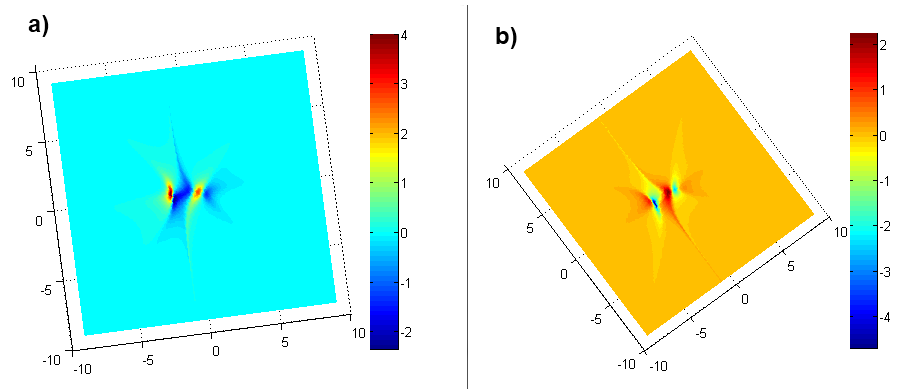
\includegraphics[width=150mm]{img/fmix_2d.png}
  \caption{2-Dimensial plots of both a) real and b) imaginary parts of nonlinear susceptibility threated as a biargumental
  function, where the color means the function value}
\end{figure}

\begin{figure} \label{fig:fmix_3d}
  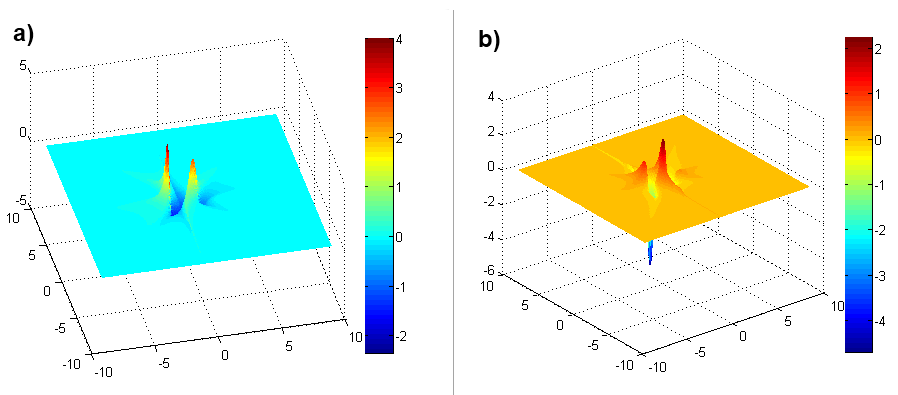
\includegraphics[width=150mm]{img/fmix_3d.png}
  \caption{3-Dimensial plots of both a) real and b) imaginary parts of nonlinear susceptibility threated as a biargumental
  function, where the color means the function value}
\end{figure}

There are dozens of models for the nonlinear optical phenomena. What is important in their derivation is to have in mind that the
frequency domain is connected with time domain with the Fourier transform.We also must remember that to build a valid model - it
must obey the causality principle in the time domain. Here from now we also will observe that the advanced models of susceptibility
does not obey the rule, that it's real (imaginary) part is an even (odd) function - we will discuss this in the next chapter.

\textit{Description of simple modification in linear model to obtain the nonlinear model}

\subsection{Derivation of the Kramers-Kronig relations for simple nonlinear model} \label{chap:problem_dnlo}

As mentioned in equation \ref{eq:polarization_volterra} in time domain polarization tensor is calculated using the leading order
term of Volterra-series. Now - when calculating the response of the system under the influence of many monochromatic light sources
- we can formulate the nonlinear multiple convolution:

\begin{equation} \label{eq:dkk_convolution}
  {P_{n, \,i}}(t)=\int \dotsi \int {G_{n, \,i, \,j_{1},\dotsc, \,j_{n}}}(t_1,\dotsc, \, t_n )\,{E_{j,
  \,1}}(t - {t_{1}})\dotsm\,{E_{j, \,n}}(t -{t_{n}})\,d{t_{1}}\,\dotsm\,d{t_{n}},
\end{equation}
where:\\
${G_{n, \,i, \,j_{1},\dotsc, \, j_{n}}}(t_1, \dotsc, \, t_n)$ - the casual n-th order Green function in
time domain.

After applying the Fourier transform to the \ref{eq:dkk_convolution} toghether with the convolution theorem we obtain:

\begin{equation} \label{eq:dkk_fapplied}
  {P_{n, \,i}}(\omega )=\int_{ - \infty }^{\infty } \dotsi\int_{ - \infty}^{\infty }{\chi_{n, \,i,
  \,{j_{1}}, \dotsc,{j_{n}}}}(\sum_{l=1}^{n}\,{\omega_{l}}, \,{\omega_{1}},\dotsc,\,{\omega_{n}
  })\,{E_{j, \,1}}({\omega_{1}})\dotsm {E_{j,\,n}}({\omega_{n}}) \, 
\end{equation}
\begin{equation*}
  \delta (\omega - (\sum_{l=1}^{n}\,{\omega_{l}}))\,d{\omega_{1}}\dotsm d{\omega_{n}}, 
  \mbox { where $\delta$ - Dirac delta   function}
\end{equation*}

The causality principle can be now assumed for each variable of the nonlinear Green function in time domain. We therefore can again
apply the Titchmarsh theorem to obtain:

\begin{equation} \label{eq:dkk_titchmarsh}
  P\,\int_{ - \infty }^{\infty }\frac {{\chi_{j, \,i, \,{j_{1}}, \dotsc, \,{j_{n}}}}(\sum_{l=1}^{n}\,
  {\Omega_{l}}, \,{\Omega_{1}},\,\dotsc, \,{\Omega_{n}})}{{\Omega_{1}} - {\omega_{1}}}
  \,d{\Omega_{1}}=i\,\pi \,{\chi_{n, \,i, \,{j_{1}},\,\dotsc \,{j_{n}}}}(\sum_{l=1}^{n}\,{\omega_{l}}, \,{\omega_{1}},
  \,\dotsc, \,{\omega_{n}})
\end{equation}

The equation \ref{eq:dkk_titchmarsh} was taken from Lucarini \cite{lucarini_kramers}. At the moment we are not sure about the
symmetry rule in case of nonlinear optics - so we propose carefully, more general that in \cite{lucarini_kramers}:

\begin{subequations}  \label{eq:derivation_lucarini}
  \begin{multline} \label{eq:dlucarini_imag}
    \Im({\chi_{n, \,i, \,{j_{1}}, \,{j_{2}}, \,\ldots,\,{j_{n}}}}(\sum_{l=1}^{n}\,{\omega_{l}}, \,{\omega_{1}}, \, {\omega_{2}},
    \,\ldots, \,{\omega_{n}})) = \\
    \frac { \dashint_{ - \infty }^{\infty }\,\dashint_{ - \infty }^{\infty}\,\ldots\,\dashint_{ - \infty }^{\infty }{
    \frac { \Re({\chi_{n, \,i, \,{j_{1}}, \,{j_{2}}, \,\ldots, \,{j_{n}}}}(\sum_{l=1}^{n}\,{\Omega_{l}}, \,{\Omega_{1}}, \,
    {\Omega_{2}}, \,\ldots, \,{\Omega_{n}}))}{({\Omega_{1}} - {\omega_{1}})\,({\Omega_{2}} - {\omega_{2}})\,\ldots\,({\Omega_{n}} -
    {\omega_{n}})} \,d{\Omega_{1}}\,d{\Omega_{2}}\,\ldots\,d{\Omega_{n}}}
    } {( - \pi )^{n}}
  \end{multline}
  \begin{multline} \label{eq:dlucarini_real}
    \Re({\chi_{n, \,i, \,{j_{1}}, \,{j_{2}}, \,\ldots, \,{j_{n}}}}(\sum_{l=1}^{n}\,{\omega_{l}}, \,{\omega_{1}}, \,{\omega_{2}},
    \,\ldots, \,{\omega_{n}})) = \\
    \frac { \dashint_{ - \infty }^{\infty }\,\dashint_{ - \infty }^{\infty}\,\ldots\,\dashint_{ - \infty }^{\infty } \frac { \Im
    ({\chi_{n, \,i, \,{j_{1}}, \,{j_{2}}, \,\ldots, \,{j_{n}}}}(\sum_{l=1}^{n}\,{\Omega_{l}}, \,{\Omega_{1}}, \, {\Omega_{2}}, \ldots,
    \,{\Omega_{n}}))}{({\Omega_{1}} - {\omega_{1}})\,({\Omega_{2}} - {\omega_{2}})\,\ldots\, ({\Omega_{n}} -
    {\omega_{n}})}\,d{\Omega_{1}}\,d{\Omega_{2}}\,\ldots\,d{\Omega_{n}}}{\pi^{n}},
  \end{multline}
\end{subequations}

We stress that by the moment we are not sure about the symetry rule for \ref{eq:dkk_titchmarsh} because in a typical nonlinear
process a response is not the instant reaction for input - and both the saturation and reflection processes takes time. When taking into consideration
only one frequency - we conclude that:

\begin{subequations}  \label{eq:derivation_conclude}
  \begin{equation}    \label{eq:dconcluse_imag}
    \Im ({\chi_{n, \,i, \,{j_{1}}, \,{j_{2}}, \, \ldots, \,{j_{n}}}}(\sum_{l=1}^{n}\,{\omega_{l}}, \,{\omega_{1}}, \, {\omega
   _{2}}, \, \ldots, \,{\omega_{n}}))= \frac {P\,\int_{ - \infty }^{\infty }\frac {\Re ({\chi_{n, \,i, \,{j_{1}}, \,{j_{2}},
    \, \ldots, \,{j_{n}}}}(\sum_{l=1}^{n}\,{\Omega_{l}}, \,{\Omega_{1}}, \,{\Omega_{2}}, \, \ldots, \,{\Omega_{n}}))}{{\Omega_{1}}
    - { \omega_{1}}}\,d{\Omega_{1}}}{ - \pi }
  \end{equation}
  \begin{equation}    \label{eq:dconslude_real}
    \Re ({\chi_{n, \,i, \,{j_{1}}, \,{j_{2}}, \, \ldots, \,{j_{n}}}}(\sum_{l=1}^{n}\,{\omega_{l}}, \,{\omega_{1}}, \,
    {\omega_{2}}, \, \ldots, \,{\omega_{n}})) = \frac {P\,\int_{ - \infty }^{\infty }\frac {\Im ({\chi_{n, \,i, \,{j_{1}},
    \,{j_{2}}, \, \ldots, \,{j_{n}}}}(\sum_{l=1}^{n}\,{\Omega_{l}}, \,{\Omega_{1}}, \,{\Omega_{2}}, \, \ldots, \,{\Omega_{n}}))}
    {{\Omega_{1}} - { \omega_{1}}}\,d{\Omega_{1}}}{\pi }
  \end{equation}
\end{subequations}

If we focus on the equations \ref{eq:derivation_lucarini} and \ref{eq:derivation_conclude} it can be seen, that they lead to the
different results. In the latter equations we are performing only one Hilbert transform for the N-dimensional array
of  $\chi_{n}, \,i, \,j_{1}, \,j_{2}, \, \ldots, \,j_{n}$. In first equation we evalute the Hilbert transform N times and also
the variables are binded within the most innter integrand, so from the numerical point of view, this multi-integral is harder to
evaluate, because we need to take into consideration the rules of calculating the multiple-level integral. In further
multi-dimensional evaluations we will use the \ref{eq:derivation_conclude} equations, because they seem to be valid. In all equations
\ref{eq:derivation_lucarini} and \ref{eq:derivation_conclude} - we forget about the symmetry rule despite of the uncertainity howto combine
it with the time-varying saturation and reflection processes. It means that the signal response does not only depend on the input
frequencies $\omega_{1},\dotsc,\omega_{n}$, but also on the time delays between them
$T_{1},\dotsc, ,T_{n-1}$:

\begin{equation} \label{eq:derive_withdelay}
   \chi_{n, \,i, \,j_{1},\dotsc,j_{n}} (\sum_{l=1}^{n}\,\omega_{l}, \,\omega_{1},\dotsc,
   \,\omega_{n}) = {\chi_{n, \,i, \,j_{1},\dotsc, \,j_{n} }}(\sum_{l=1}^{n}\,\omega_{l}, \,\omega_{1},\dotsc, 
   \, \omega_{n}, \,T_{1}, \dotsc, \,T_{N-1})
 \end{equation}

Automatically we expand \ref{eq:derivation_conclude} into (2.4.7a-b)

\begin{subequations} \label{eq:dconlude_expand}
  \begin{multline}   \label{eq:dcexpand_imag}
    \Im ({\chi_{n, \,i, \,j_{1}, \,j_{2}, \, \ldots, \, j_{n}}} (\sum_{l=1}^{n}\,\omega_{l}, \, \omega_{1}, \,\omega_{2},
    \, \ldots, \,\omega_{n}, \,T_{1}, \,T_{2}, \, \ldots, \, T_{n - 1})) = \\
    \frac{\dashint_{ - \infty }^{\infty } \frac {\Re
    ({\chi_{n, \,i, \,j_{1 }, \,j_{2}, \, \ldots, \,j_{n}}}(\sum_{l=1}^{n} \,\Omega_{l}, \, \Omega_{1}, \, \Omega_{2}, \,\ldots,
    \, \Omega_{n}, \,T_{1}, \,T_{2}, \,\ldots , \,T_{n - 1}))}{\Omega_{1} - \omega_{1}}\,d{\Omega_{1}}}{ - \pi }
  \end{multline}
  \begin{multline}   \label{eq:dcexpand_real}
    \Re ({\chi_{n, \,i, \,j_{1}, \,j_{2}, \, \ldots, \,j_{n}}}(\sum_{l=1}^{n}\,\omega_{l}, \,\omega_{1}, \, \omega_{2},
    \, \ldots, \, \omega_{n}, \,T_{1}, \, T_{2}, \, \ldots, \, T_{N - 1})) = \\
    \frac{\dashint_{-\infty}^{\infty}\frac{\Im
    ({\chi_{n, \,i, \,j_{1 }, \,j_{2}, \, \ldots, \,j_{n}}}(\sum_{l=1}^{n} \,\Omega_{l}, \,\Omega_{1}, \,\Omega_{2},
    \,  \ldots, \,\Omega_{n}, \,T_{1}, \,T_{2}, \, \ldots, \, T_{n - 1}))}{\Omega_{1} - \omega_{1}} \,d{\Omega_{1}}}{\pi }
  \end{multline}
\end{subequations}

One might say that this equations are to general to practically use them - but for our point of view it is important that in the
nonlinear case we do not need to integrate from zero to plus infinity but through the full real line - we will keep this assumption
in all further nonlinear calculations.

\textit{Mathematical derivation of the Kramers-Kronig relations for simple nonlinear model.}

\subsection{Overview of the simple quantum-perturbative model} \label{chap:problem_quantum}

We are interested in derivation of the first-order linear susceptibility and the second-order and third-order nonlinear
susceptibility using the quantum mechanical approach and by solving the Schrödinger equation. While this is the cutting edge, most
investigated area of moderd physics and an difficult mathematics area - we will only try to do the hand-waving introduction into
this matter. What is important in this model, by Boyd \cite{boyd_nlo} that in case of nonlinear optics the important relaxation
process is not taken into account. As we have written before, the nonlinear susceptibilities depend not only on the input wave
frequency but also on the time between those impulses - we should try the quantum-perturbative model as not yet finalized.


The general assumption in the quantum mechanics applied for nonlinear optics is that the whole material properties can be described
using the time-dependent Schrödinger equation:

\begin{equation} \label{eq:schroedinger_equation}
  i\,\hbar\,({\frac {\partial }{\partial t}}\,\psi (r, \,t))=H\, \ket{ \psi(r, \,t) },
\end{equation}

where: 

\begin{tabular}{ r l}
  H & - Hamiltonian operator \\
  $\ket{\psi(r,\,t)}$ & - atomic wavefunction \\
\end{tabular}


The H Hamiltonian can be splitted:

\begin{equation} \label{eq:schroedinger_hamiltonian}
  H={H_{0}} + {V_{t}},
\end{equation}

where:

\begin{tabular} {r l}
  ${H_{0}}$ & - Hamiltonian for free atom \\
  ${V_{t}}$ & - Hamiltonian for interaction of an atom with electromagnetic field \\
\end{tabular}


Hence the \ref{eq:schroedinger_equation} equation is hard to solve exactly, we replace the H Hamiltonian with:

\begin{equation} \label{eq:shamiltionian_replaced}
  H = {H_{0}} + \lambda \,{V_{t}},
\end{equation}

where: 

\begin{tabular} {r l}
  $\lambda \,\ in \,C[0, 1]$ & - perturbative parameter that describes the strength of interaction. 
\end{tabular}



Not jumping into details, we may now try to find a solution to Schrödinger's equation with power the following power series:

\begin{equation} \label{eq:schrodinger_solution}
  \ket{\psi (r, \,t) } = \ket{ \psi_{0}(r, \,t)} + \lambda \,\ket{\psi_{1}(r, \,t)} + \lambda^{2}\,\ket{\psi_{2}(r, \,t) } +
  \ldots
\end{equation}

With such an perturbative assumption we can now modify the initial \ref{eq:schroedinger_equation} into a form:

\begin{subequations} \label{eq:schrodinger_modified}
  \begin{equation}   \label{eq:smodified_zero}
    i\,\hbar\,({\frac {\partial }{\partial t}}\,\psi_{0}(r, \,t)) = H_{0}\, \ket{\psi_{0}(r, \,t)}
  \end{equation}
  \begin{equation}   \label{eq:smodified_n}
    i\,\hbar\,({\frac {\partial }{\partial t}}\,\psi_{n}(r, \,t)) = H_{0}\,( \ket{\psi_{n}(r, \,t)} +
    \mathrm{V}(t)\,\ket{\psi_{n-1}(r, \,t)})
  \end{equation}
\end{subequations}

We call the $\ket{{\psi_{n}}(r, \,t)}$ an eigenvector. They can be expanded in terms of unperturbed states as following:

\begin{equation} \label{eq:schrodinger_unperturbed}
  {\psi_{n}}(r, \,t)=\sum_{l}\,{a_{N, \,l}}(t)\,{u_{l}}(r)\,e^{( - i\,{\omega_{l}}\,t)}
\end{equation}

where: $a_{N,\,l}(t)$ - amplitude of the probability that the atom is in energy eigenstate l at time l to the Nth order in
perturbation.


We next find that:
\begin{equation} \label{eq:schrodinger_totaldiff}
  \dot a_{N, \,m}(t) = \frac {\sum_{l} \, a_{N-1, \, l}(t) \, V_{ml}(t) \, e^{(-i\, \omega_{ml} \,t)}}{i \, \hbar},
\end{equation}


where: 

\begin{tabular}{ r l}
  $ \omega_{ml}$ &= $\omega_{m} - \omega_{l}$ \\
  $V_{ml}$ &= $\langle {u_{m}}\, | \,\mathrm{V}(t)\, | \,u_{l}\rangle $ \\
\end{tabular}

When we integrate \ref{eq:schrodinger_totaldiff} we get:

\begin{equation} \label{eq:stotaldiff_afterintegrate}
   a_{N, \,l}(t) = \frac{1}{\hbar \, i} \sum_{l}\,\int_{ -\infty }^{t} V_{ml} (T)\, a_{N-1, \,l}(T)\,e^{(i\,\omega_{ml}}\,T)\,dT
\end{equation}

From such probability amplitude we will extract the explicit form for the linear, second-order and third-order optical
susceptibilities. Here we will provide two more physical representations:

\begin{subequations} \label{eq:more_representations}
  \begin{equation}   \label{eq:mreps_dipole}
    \mathrm{V}(t)= - \mu \,{E_{x}}(t) \mbox{ ($mu$ - electric dipole moment operator)}
  \end{equation}
  \begin{equation}   \label{eq:mreps_optical}
    {E_{x}}(t)=\sum_{p}\,\mathrm{E}({\omega_{p}})\,e^{( - i\,{\omega_{p}}\,t)} \mbox{ ( ${E_{x}}(t)$ - total optical field ) }
  \end{equation}
\end{subequations}

Now it is possible to assume that the linear, second-order and third-order of the probability amplitude equals:

\begin{subequations} \label{eq:probability_amplitude}
  \begin{equation}   \label{eq:pamplitude_linear}
    a_{1, \,m}(t) = \frac {1}{h} \sum_{p}\,\frac {{\mu_{mg}}\,\mathrm{E}({\omega_{p}})}{{\omega_{mg}} - {\omega_{p}}}
    e^{(i\,({\omega_{mg}} - {\omega_{p}})\,t)}
  \end{equation}
  \begin{equation}   \label{eq:pamplitude_quadratical}
    {a_{2, \,n}}(t) = \frac {1}{h^{2}}\sum_{pq}\, \left(  \! \sum_{m}\,\frac {{\mu_{nm}}\,\mathrm{E}({\omega_{q}})\, {\mu_{mg}}\,
      \mathrm{E}({\omega_{p}})}{({\omega_{ng}} - {\omega_{p}} - {\omega_{q}})\,({\omega_{mg}} - {\omega_{p}})\,({\omega_{mg}} -
      \omega_{p})} \! \right) e^{(i\,({\omega_{mg}} - {\omega_{p}} - {\omega_{q}})\,t)}
  \end{equation}
  \begin{equation}   \label{eq:pamplitude_cubic}
     {a_{3, \,n}}(t)=\frac {1}{h^{3}} \sum_{pqr}\, \left(  \! \sum_{mn}\,\frac {{
       \mu_{vn}}\,\mathrm{E}({\omega_{r}})\,{\mu_{nm}} \,\mathrm{E}({\omega_{q}})\,{\mu_{mg}}\,\mathrm{E}({\omega_{p}})\,1}
       {({\omega_{vg}} - {\omega_{p}} - { \omega_{q}} - {\omega_{r}})\,({\omega_{ng}} - {\omega_{p}} - {\omega_{q}}) \, ({\omega
      _{mg}} - {\omega_{p}} )} \!  \right) e^{(i\,({\omega_{vg}} - {\omega_{p}} - {\omega_{q}}- {\omega_{r}})\,t)}
  \end{equation}
\end{subequations}


respectively. This results will lead us to the following results about the optical susceptibilities:


\begin{subequations} \label{eq:susceptibility_results}
  \begin{equation}   \label{eq:sresults_linear}   
    {\chi_{1, \,i, \,j}}({\omega_{p}}) = \frac {N}{{\varepsilon_{0}}\,h} \sum_{m}\,(\frac {{\mu_{i, \,gm}}\,{\mu_{j, \,
     mg}}}{{\omega_{mg}} - {\omega_{p}}} + \frac {{\mu_{j, \,gm}}\,{\mu_{i, \,mg}}}{{\omega_{mg}} + {\omega_{p}}})
  \end{equation}
  \begin{equation}   \label{eq:sresults_quadratical}
     \chi_{2, \,i, \,j, \,k}({\omega_{p}} + {\omega_{q}}, \,{\omega_{q}}, \,{\omega_{p}}) = 
      \frac{N}{{\varepsilon_{0}}\,h^{2}}{P_{I}}\, \sum_{mn}\, (
      \frac{{\mu_{i,\,gn}}\,{\mu_{j,\,nm}}\,{\mu_{k,\,mg}}}{(\omega_{ng} - \omega_{p} - {\omega_{q}})\,({ \omega_{mg}}
      -{\omega_{p}})} + \\ 
  \end{equation}
  \begin{alignat*} {1}
    &  + \frac{{\mu_{j,\,gn}}\,{\mu_{i,\,nm}}\,{\mu_{k,\,mg}}}{(\omega_{ng} + \omega_{q})\,(\omega_{mg} - \omega_{p})}
       + \frac{{\mu_{i,\,gn}}\,{\mu_{k,\,nm}}\,{\mu_{i,\,mg}}}{(\omega_{ng} + \omega_{q})\,(\omega_{mg} + \omega_{p}
       + \omega_{q})}),\nonumber\\  
    & \mbox{ \footnotesize{where $P_{I}$  denotes the intrinsic permutation operator} } \nonumber
  \end{alignat*}
  \begin{equation} \label{eq:sresults_cubic}   
   {\chi_{3, \,k, \,j, \,i, \,h}}({\omega_{\sigma }}, \,{\omega_{r}}, \,{\omega_{q}}, \,{\omega_{p}}) =
   \end{equation}
  \begin{alignat*}{1} 
    & \frac{N}{{\varepsilon_{0}}\,h^{3}} {P_{I}} \! \sum_{mnv}\,(\frac {{\mu_{k, \,gv}}\,{\mu_{j, \,vn}}\,{\mu_{i,
    \,nm}}\,{\mu_{h, \,mg}}} {({\omega_{vg}} - {\omega_{r}} - {\omega_{q}} - {\omega_{p}})\,({\omega_{ng}} - {\omega_{q}} - {\omega_{p}})\,({\omega_{mg}} - { \omega_{p}})} 
    \\ &  + \frac {{\mu_{j, \,gv}}\,{\mu_{k, \,vn}}\,{\mu_{i, \,nm}}\,{\mu_{h, \,mg}}}
    {({\omega_{vg}} + {\omega_{r}}) \,({\omega_{ng}} - {\omega_{q}} - {\omega_{p}})\,({\omega_{ mg}} - {\omega_{p}})} 
         + \frac {{\mu_{j, \,gv}}\,{\mu_{i, \,vn}}\,{\mu_{k, \,nm}}\,{\mu_{h, \,mg}}}
    {({\omega_{vg}}+{\omega_{r}})\,({\omega_{ng}} + {\omega_{r}} + {\omega_{q}})\,({\omega_{mg}} - {\omega_{p}})}  \nonumber
    \\ &  + \frac {{\mu_{j, \,gv}}\,{\mu_{i, \,vn}}\,{\mu_{h,\,nm}}\,{\mu_{k, \,mg}}}
    {({\omega_{vg}} + {\omega_{r}})\,({\omega_{ng}} + {\omega_{r}} + {\omega_{q}} )\,({\omega_{mg}} + {\omega_{r}} + {\omega_{q}} + { \omega_{p}})})
    \nonumber
  \end{alignat*}
\end{subequations}


Derivation and equation details may be found in Kuzyk \cite{kuzyk_nlo} and Boyd \cite{boyd_nlo}. The
\ref{eq:susceptibility_results} are sometimes called the sum-over-states euqations, because we are performing the sum over all
possible excited states of the atom. Using the another physical model - called the density matrix operator, we can obtain another
set of equations which are a slight modifications of \ref{eq:susceptibility_results}:


\begin{subequations} \label{eq:susceptibility_sligh_modifications}
  \begin{equation} \label{eq:ssmods_linear}
    {\chi_{1}}({\omega_{p}})=\frac {N}{{\varepsilon_{0}}\,h}\sum_{n}\,(\frac {{\mu_{i, \,an}}\,{\mu_{j, \,na}}}{{\omega_{na}} -
    {\omega_{p}} - i\,{\gamma_{na}}} + \frac {{\mu_{i, \,na}}\,{\mu_{j, \,an}}}{{\omega_{na}} - {\omega_{p}} + i\,{\gamma_{na}}})
  \end{equation}
  \begin{equation} \label{eq:ssmods_quadratical}
    {\chi_{2, \,i, \,j, \,k}}({\omega_{p}} + {\omega_{q}}, \,{\omega_{q}}, \,{\omega_{p}}) = \frac
    {N}{2\,{\varepsilon_{0}}\,h^{2}}\sum_{lmn}\,{\rho_{0, \,ll}}\,(\frac {{\mu_{i, \,l, \,n}}\,{\mu_{j, \,nm}}\,{\mu_{k,
    \,ml}}}{({\omega_{nl}} - {\omega_{p}} - {\omega_{q}}- i\,{\gamma_{nl}})\,({\omega_{ml}} - {\omega_{p}} - i\,{\gamma_{ml}})} +
  \end{equation}
  \begin{alignat*}{1}
    + \frac {{\mu_{i, \,l, \,n}}\,{\mu_{k, \,nm}}\,{\mu_{j, \,ml}}}
     {({\omega_{nl}} - {\omega_{p}} - {\omega_{p}} - i\,{\gamma_{nl}})\,({\omega_{ml}} - {\omega_{q}} - i\,{\gamma_{ml}})} 
+\\ +\frac {{\mu_{k, \,l, \,n}}\,{\mu_{i, \,nm}}\,{\mu_{j,\,ml}}}
     {({\omega_{mn}} - {\omega_{p}} - {\omega_{q}} - i\,{\gamma_{mn}})\,({\omega_{nl}} + {\omega_{q}} + i\,{\gamma_{nl}})}
     \nonumber
+\\ +\frac{{\mu_{j, \,l, \,n}}\,{\mu_{i, \,nm}}\,{\mu_{k, \,ml}}}
     {({\omega_{mn}} - {\omega_{p}} - {\omega_{q}} - i\,{\gamma_{mn}})\,({\omega_{nl}} + {\omega_{q}} + i\,{\gamma_{nl}})} 
+\\ +\frac {{\mu_{j, \,l, \,n}}\,{\mu_{i, \,nm}}\,{\mu_{k,\,ml}}}
     {({\omega_{nm}} + {\omega_{p}} + {\omega_{q}} + i\,{\gamma_{nm}})\,({\omega_{ml}} - {\omega_{p}} - i\,{\gamma_{ml}})}
     \nonumber
+\\ +\frac{{\mu_{k, \,l, \,n}}\,{\mu_{j, \,nm}}\,{\mu_{i, \,ml}}}
     {({\omega_{nm}} + {\omega_{p}} + {\omega_{q}} + i\,{\gamma_{nm}})\,({\omega_{ml}} - {\omega_{p}} - i\,{\gamma_{ml}})} 
+\\ +\frac {{\mu_{k, \,l, \,n}}\,{\mu_{j, \,nm}}\,{\mu_{i, \,ml}}}
     {({\omega_{ml}} + {\omega_{p}} + {\omega_{q}} + i\,{\gamma_{ml}})\,({\omega_{nl}} + {\omega_{p}} + i\,{\gamma_{nl}})}
     \nonumber
+\\ +\frac {{\mu_{j, \,l, \,n}}\,{\mu_{k, \,nm}}\,{\mu_{i, \,ml}}}
     {({\omega_{ml}} + {\omega_{p}} + {\omega_{q}} + i\,{\gamma_{ml}})\,({\omega_{nl}} + {\omega_{q}} + i\,{\gamma_{nl}})})
     \nonumber
  \end{alignat*}
  \begin{equation} \label{eq:ssmods_cubic}
    {\chi_{3, \,k, \,j, \,i, \,h}}({\omega_{p}} + {\omega_{q}} + {\omega_{r}}, \,{\omega_{r}}, \,{\omega_{q}}, \,{\omega_{p}})=\frac
	{N}{{\varepsilon_{0}}\,h^{3}}\,\cdot
  \end{equation}
  \begin{alignat*}{1}
  	\cdot\,\sum_{vnml}\,{\rho_{0, \,ll}}\,(
  	\frac {{\mu_{k,\,lv}}\,{\mu_{j,\,vn}}\,{\mu_{i,\,nm}}\,{\mu_{h,\,ml}}}
  	 {({\omega_{vl}} - {\omega_{p}} - {\omega_{q}} - {\omega_{r}} - i\,{\gamma_{vl}})\,
  	  ({\omega_{nl}} - {\omega_{p}} - {\omega_{q}} - i\,{\gamma_{nl}})\,
  	  ({\omega_{ml}} - {\omega_{p}} - i\,{\gamma_{ml}})} 
+\\ +\frac {{\mu_{h,\,lv}}\,{\mu_{k,\,vn}}\,{\mu_{j,\,nm}}\,{\mu_{i,\,ml}}}
     {({\omega_{nv}} - {\omega_{p}} - {\omega_{q}} - {\omega_{r}} - i\,nv)\,
      ({\omega_{mv}} -	{\omega_{p}} - {\omega_{q}} - i\,{\gamma_{mv}})\,
      ({\omega_{vl}} + {\omega_{p}} + i\,{\gamma_{vl}})} 
+\\ +\frac {{\mu_{i,\,lv}}\,{\mu_{k,\,vn}}\,{\mu_{j,\,nm}}\,{\mu_{h,\,ml}}}
     {({\omega_{nv}} - {\omega_{p}} - {\omega_{q}} - {\omega_{r}} - i\,{\gamma_{nv}})\,
      ({\omega_{vm}} + {\omega_{p}} + {\omega_{q}} + i\,{\gamma_{vm}})\,
      ({\omega_{ml}} - {\omega_{p}} - i\,{\gamma_{ml}})} 
+\\ +\frac {{\mu_{h,\,lv}}\,{\mu_{i,\,vn}}\,{\mu_{k,\,nm}}\,{\mu_{j,\,ml}}}
     {({\omega_{mn}} - {\omega_{p}} - {\omega_{q}} - {\omega_{r}} - i\,{\gamma_{mn}})\,
      ({\omega_{nl}} - {\omega_{p}} - {\omega_{q}} + i\,{\gamma_{nl}})\,
      ({\omega_{vl}} + {\omega_{p}} + i\,{\gamma_{vl}})} 
+\\ +\frac {{\mu_{j,\,lv}}\,{\mu_{k,\,vn}}\,{\mu_{i,\,nm}}\,{\mu_{h,\,ml}}}
     {({\omega_{vn}} - {\omega_{p}} - {\omega_{q}} - {\omega_{r}} + i\,{\gamma_{vn}})\,
      ({\omega_{nl}} - {\omega_{p}} - {\omega_{q}} - i\,{\gamma_{nl}})\,
      ({\omega_{ml}} - {\omega_{p}} - i\,{\gamma_{ml}})} 
+\\ +\frac {{\mu_{h,\,lv}}\,{\mu_{j,\,vn}}\,{\mu_{k,\,nm}}\,{\mu_{i,\,ml}}}
     {({\omega_{nm}} + {\omega_{p}} + {\omega_{q}} + {\omega_{r}} + i\,{\gamma_{nm}})\,
      ({\omega_{mv}} - {\omega_{p}} - {\omega_{q}} - i\,{\gamma_{mv}})\,
      ({\omega_{vl}} + {\omega_{p}} + i\,{\gamma_{vl}})} 
+\\ +\frac {{\mu_{i,\,lv}}\,{\mu_{j,\,vn}}\,{\mu_{k,\,nm}}\,{\mu_{h,\,ml}}}
     {({\omega_{vm}} + {\omega_{p}} + {\omega_{q}} + {\omega_{r}} + i\,{\gamma_{nm}})\,
      ({\omega_{vm}} + {\omega_{p}} + {\omega_{q}} + i\,{\gamma_{mv}})\,
      ({\omega_{ml}} - {\omega_{p}} - i\,{\gamma_{ml}})} 
+\\ +\frac {{\mu_{h, \,lv}}\,{\mu_{i,\,vn}}\,{\mu_{j,\,mn}}\,{\mu_{k,\,ml}}}
     {({\omega_{ml}} + {\omega_{p}} + {\omega_{q}} + {\omega_{r}} + i\,{\gamma_{ml}})\,
      ({\omega_{nl}} + {\omega_{p}} + {\omega_{q}} + i\,{\gamma_{nl}})\,
      ({\omega_{vl}} + {\omega_{p}} + i\,{\gamma_{vl}})})
  \end{alignat*}
\end{subequations}

What is interesting that after expading all the permutations in \ref{eq:susceptibility_sligh_modifications} we will get the 48
different summands - which shows how the quantum mechanical approach is hard to understand. The important difference between
\ref{eq:susceptibility_results} and \ref{eq:susceptibility_sligh_modifications} equations is that we add the imaginary
${\gamma_{ab}}$ element which describes the damping rate of ${p_{ab}}$ - which is an element of an density matrix, describing the
coherence between states a and b: ${\rho_{ab}}=\langle a\, | \,{\rho_{x}}\, | \,b \rangle, $ where: ${\rho_{x}}$ - density
operator.

In further calculations we will use the both the \ref{eq:susceptibility_results} and \ref{eq:susceptibility_sligh_modifications}
equations in simplified version - with few summands only.

A typical results obtained with equations \ref{eq:susceptibility_sligh_modifications} are shown in the figure \ref{fig:qp_plot}:

\begin{figure} 
  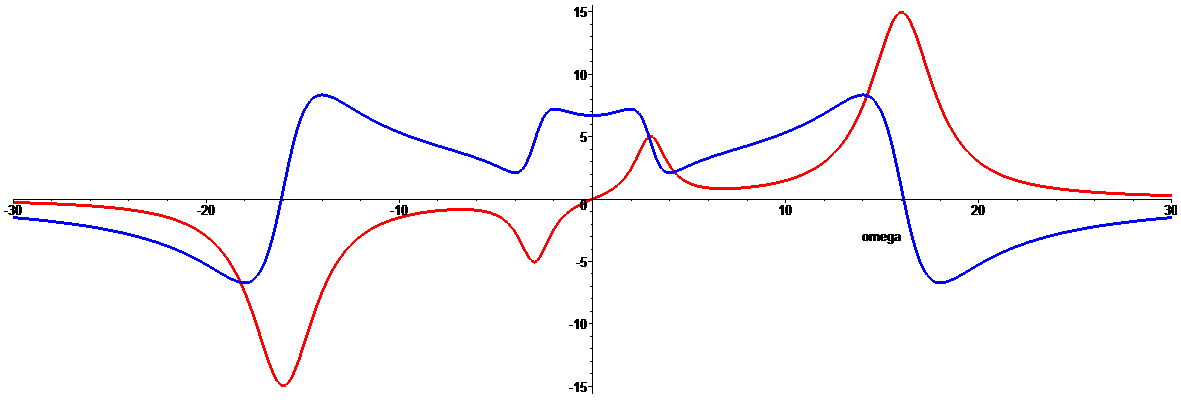
\includegraphics[width=150mm]{img/qp_plot.png}
  \caption{Quantum-perturbative plot for 3-level model of with arbitrary (non-physical) parameters. Red plot is for the imaginary
  and the blue plot is for the real part on linear susceptibility.
  \label{fig:qp_plot}}
\end{figure}
\begin{figure} 
  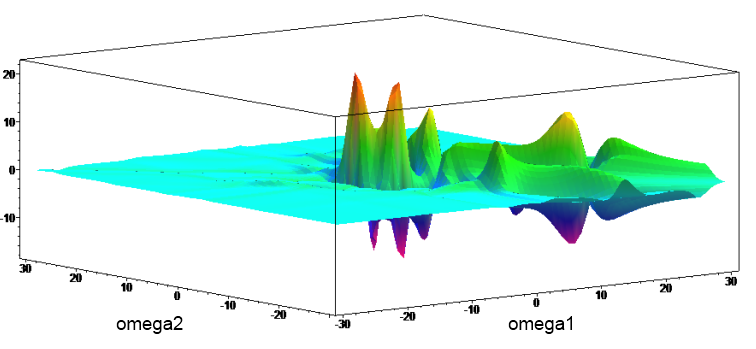
\includegraphics[width=150mm]{img/qp_3da.png} \\
  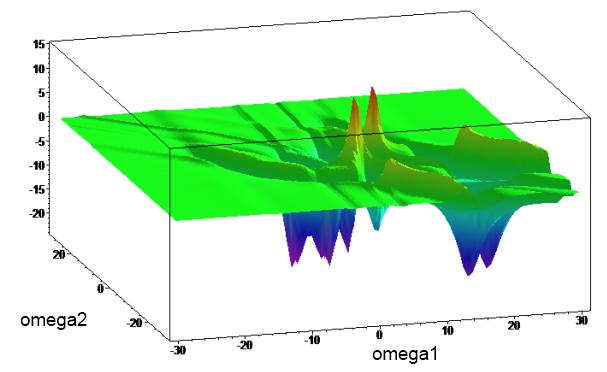
\includegraphics[width=150mm]{img/qp_3db.png}
  \caption{Quantum-perturbative plot for 3-level model of with arbitrary (non-physical) parameters. Red plot is for the imaginary
  and the blue plot is for the real part on second-order susceptibility.
  \label{fig:qp_3d}}
\end{figure}
  
\textit{brief overview of the perturbative model}

\subsection{Derivation of the Kramers-Kronig relations for a sim\-ple qua\-ntum-per\-tur\-ba\-tive model}
\label{chap:problem_dquantum}

Using the \ref{eq:derivation_lucarini} for the just showed model - we will connect the real and imaginary part of
quantum-perturbative derived optical susceptibilities using the Hilbert transform form:

\begin{subequations} \label{eq:quantum_derivation1}
  \begin{equation}   \label{eq:qderiv1_real}
    \Re  \left(  \! {\chi_{1, \,j, \,k}}({\omega_{p}}) \!  \right) = \frac {1}{\pi }\dashint_{ -\infty }^{\infty }\frac {\Im
    ({\chi_{1, \,j, \,k}}(\Omega ))}{\Omega  - {\omega_{p}}}\,d\Omega
  \end{equation}
  \begin{equation}   \label{eq:qderiv1_imag}
    \Im  \left(  \! {\chi_{1, \,j, \,k}}({\omega_{p}})\!  \right) = \frac {1}{-\pi }\dashint_{ -\infty }^{\infty }\frac {\Re
    ({\chi_{1, \,j, \,k}}(\Omega ))}{\Omega  - {\omega_{p}}}\,d\Omega  
  \end{equation}
\end{subequations}

\begin{subequations} \label{eq:quantum_derivation2}
  \begin{equation}   \label{eq:qderiv2_real}
    \Re  \left(  \! {\chi_{2, \,i, \,j, \,k}}({\omega_{p}} + {\omega_{q}}, \,{\omega_{p}}, \,{\omega_{q}})\!  \right)=\frac
    {1}{\pi} \dashint_{ - \infty }^{\infty }\dashint_{ - \infty }^{\infty }\frac {\Im ({ \chi_{2, \,i, \,j, \,k}}({\Omega_{p}} +
    {\Omega_{q}}, \,{\Omega_{p}}, \,{\Omega_{q}}))}{({\Omega_{p}} - {\omega_{p}}) \,({\Omega_{q}} -
    {\omega_{q}})}\,d{\Omega_{p}}\,d{\Omega_{q} }
  \end{equation}
  \begin{equation}   \label{eq:qderiv2_imag}
      \Im  \left(  \! {\chi_{2, \,i, \,j, \,k}}({\omega_{p}} + {\omega_{q}}, \,{\omega_{p}}, \,{\omega_{q}})\!  \right)=\frac{1}{ -
      \pi } \dashint_{ - \infty }^{\infty }\dashint_{ - \infty }^{\infty }\frac {\Re ({ \chi_{2, \,i, \,j, \,k}}({\Omega_{p}} +
      {\Omega_{q}}, \,{\Omega_{p}}, \,{\Omega_{q}}))}{({\Omega_{p}} - {\omega_{p}}) \,({\Omega_{q}} -
      {\omega_{q}})}\,d{\Omega_{p}}\,d{\Omega_{q} }
  \end{equation}
\end{subequations}

\begin{subequations} \label{eq:quantum_derivation3}
  \begin{equation}   \label{eq:qderiv3_real}
    \Re  \left(  \! {\chi_{3, \,i, \,j, \,k, \,l}}({\omega_{p}} + {\omega_{q}} + {\omega_{r}}, \,{\omega_{p}}, \,{\omega_{q}},
    \,{\omega_{r}}) \!  \right)=
  \end{equation}
  \begin{alignat*}{1}
   = \frac{1}{\pi} \dashint_{ - \infty }^{\infty }\dashint_{ - \infty }^{\infty }\dashint_{ - \infty
    }^{\infty }\frac {\Im ({\chi_{3, \,i, \,j, \,k, \,l}}({\Omega_{p}} + {\Omega_{q}} + {\Omega_{r}}, \,{\Omega_{p}}, \,{\Omega_{q}},
    \,{\Omega_{r}}))}{({ \Omega_{p}} - {\omega_{p}})\,({\Omega_{q}} - {\omega_{q}})\,( {\Omega_{r}} -
    {\omega_{r}})}\,d{\Omega_{p}}\,d{\Omega_{q}}\, d{\Omega_{r}}
  \end{alignat*}
  \begin{equation}   \label{eq:qderiv3_imag}
    \Im  \left(  \! {\chi_{3, \,i, \,j, \,k, \,l}}({\omega_{p}} + {\omega_{q}} + {\omega_{r}}, \,{\omega_{p}}, \,{\omega_{q}},
    \,{\omega_{r}}) \!  \right)=
  \end{equation}
  \begin{alignat*}{1}
  = \frac{1}{ - \pi } \dashint_{ - \infty }^{\infty }\dashint_{ - \infty }^{\infty
    }\dashint_{ - \infty }^{\infty }\frac {\Im ({\chi_{3, \,i, \,j, \,k, \,l}}({\Omega_{p}} + {\Omega_{q}} + {\Omega_{r}},
    \,{\Omega_{p}}, \,{\Omega_{q}}, \,{\Omega_{r}}))}{({ \Omega_{p}} - {\omega_{p}})\,({\Omega_{q}} - {\omega_{q}})\,( {\Omega_{r}}
    - {\omega_{r}})}\,d{\Omega_{p}}\,d{\Omega_{q}}\, d{\Omega_{r}}
  \end{alignat*}
\end{subequations}

In further chapters we will put this equations into some numerical evaluations.

\footnotesize \textit{Mathematical derivation of the Kra\-mers-Kro\-nig re\-la\-tions for sim\-ple per\-tur\-ba\-ti\-ve model.}

\subsection{Overview of the other models} \label{chap:problem_other}


D. C. Hutchings et al. \cite{hutchings_kramers2} have proposed the models for particular nonlinear absorption processes as
following: Here we would like to state  - only from the physical point of view - without formulating advanced mathematical models -
that the theory of K-K relations - or to say it precisely - the conjugated pairs of Hilbert transforms - need to be structured and
defined generaly for both the linear and nonlinear case - there must be on valid theory - it is not a good situation - when we
start from one theory and then ''modify'' it for some extra case - because it leads to misunderstanding in general. As the title of
this thesis contains the word - understanding - we should at least try to express a new, general theory of optical phenomena -
because it is ''only and even'' - the interaction of a chemical molecules with incoming photons in short or long period of time.

\begin{equation} \label{eq:other_tpa}
  \mbox{Two photon absorption: } F_{TPA} ({x_{1}}, \,{x_{2}}) = \frac {({x_{1}} + {x_{2}} - 1)^{(\frac {3}{2})}\,(\frac
  {1}{{x_{1}}} + \frac {1}{{x_{2}}}) ^{2}} {2^{7}\,{x_{1}}\,{x_{2}}^{2}}
\end{equation}
\begin{equation} \label{eq:other_raman}
  \mbox{Raman: } {F_{R}}({x_{1}}, \,{x_{2}})=\frac {({x_{1}} - {x_{2}} - 1)^{(\frac {3}{2})}\,(\frac {1}{{x_{1}}} - \frac
  {1}{{x_{2}}})^{2}}{2^{7}\,{x_{1}}\,{x_{2}}^{2}}
\end{equation}
\begin{equation} \label{eq:other_lstark}
  \mbox{Linear stark: } {F_{LS}}({x_{1}}, \,{x_{2}})= - \frac {({x_{1}} - 1)^{(\frac {3}{2})}}{2^{6}\,{x_{1}}\,{x_{2}}^{2}} \frac
  {1}{{x_{2}}^{2}}
\end{equation}
\begin{equation} \label{eq:other_qstark}
  \mbox{Quadratic stark: } {F_{QS}}({x_{1}}, \,{x_{2}})= - \frac {1\,(\frac {1}{{x_{1}} - {x_{2}}} + \frac {1}{{x_{1}} +
  {x_{2}}})}{2^{10}\, {x_{1}}\,{x_{2}}^{2}\,({x_{1}} - 1)^{(\frac {1}{2})}}
\end{equation}

Where in all \ref{eq:other_tpa} \ref{eq:other_raman} \ref{eq:other_lstark} and \ref{eq:other_qstark} equations we assume that:
${x_{1}}=\frac {\hbar\,{\omega_{1}}}{{E_{g}}}$, ${x_{2}}=\frac {h\,{\omega_{2}}}{{E_{g}}}$, where: ${E_{g}}$ - the edge absorption
energy, a nonconstant parameter.

\textit{Introduction into variety of other models avaiable in physics of the nonlinear optics}

\textbf{Should I write more on particular models?}

\subsection{Derivation of the Kramers-Kronig relations for other models} \label{chap:problem_dother}


D. C. Hutchings et al. \cite{hutchings_kramers2} have also proposed the analytical equations based on \ref{eq:other_tpa}
\ref{eq:other_raman} \ref{eq:other_lstark} and \ref{eq:other_qstark} aquired with Hilbert transform:


\begin{equation} \label{eq:hother_euqation}
  \mathrm{G}(x)=\frac {P\,\int_{ - \infty }^{\infty }\frac { \mathrm{F}(y, \,x)}{y - x}\,dy}{\pi }
\end{equation}

And they obtained the following results:

\begin{equation} \label{eq:dother_tpa}
  \mbox{Two photon absorption: } {G_{TPA}}(x) = (2\,x)^{6}\,\cdot
\end{equation}
\begin{alignat*}{1}
  \cdot\,[-\frac {3}{8}\,x^{2}(1 - x)^{( - \frac {1}{2})} + 3x(1 - x)^{(\frac
  {1}{2})} - 2(1 - x)^{(\frac {3}{2})} + 2\Theta (1 - 2\,x)(1 - 2\,x)^{(\frac {3}{2})}], 
\end{alignat*}
( where $\Theta (t)$ - Heaviside function)
\begin{equation} \label{eq:dother_raman}
  \mbox{Raman: } {G_{R}}(x) = [1/(2\,x)^{6}][-\frac {3}{8}x^{2}(1 + x)^{( - \frac {1}{2})} - 3x(1 + x)^{(\frac {1}{2})}-2(1 +
  x)^{(\frac {3}{2})}+2(1 + 2\,x)^{(\frac {3}{2})}]
\end{equation}
\begin{equation} \label{eq:dother_lstark}
  \mbox{Linear stark: } {G_{LS}}(x) = [1/(2\,x)^{6}][2 - (1 - x)^{(\frac {3}{2})} - (1 + x)^{(\frac {3}{2})}]
\end{equation}
\begin{equation} \label{eq:dother_qstark}
  \mbox{Quadratic stark: } {G_{QS}}(x) = [1/(2^{10}x^{5})]\,\cdot
\end{equation}
\begin{alignat*}{1}
  \cdot\,[(1 - x)^{( - \frac {1}{2})} - (1 + x)^{( - \frac {1}{2})} - \frac {1\,x\,(1 - x)^{(\frac {3}{2})}}{2} - \frac {1\,x\,(1 +
  x) ^{( - \frac {3}{2})}}{2}]
\end{alignat*}

In further chapters we will put this equations into a try. There can be other models found in literature - but our approach will
remaind the same - check if the model assumed is valid.

\textit{The derived models using the Hilbert transform are presented}

\section{Z-scan Measurments (understanding)} \label{chap:zscan}

\subsection{Overview of the z-scan technique} \label{chap:zscan_overview}

One of the most important questions being the major motivation of this thesis is how the theory of Hilbert transform or the
Kramers-Kronig relations can be applied to the data measured with the standard ''open aperture'' and ''closed aperture'' z-scan
technique. In this chapter we will describe the process of data collection and its translation into the nonlinear absorption
coefficient spectra and nonlinear refraction index spectra. As mentioned before, since summer 2010 we have set up the femtosecond
z-scan system using a Quantronix Integra regenerative amplifier operating at 1 kHz and providing appr. 1 mJ, 100 fs, 800 nm
pulses. It is used as a pump to the Palitra optical parametric amplifier, which, using several different frequency mixing schemes,
can provide the coverage of the 450 - 2000 nm wavelength range. The best way to describe this set up will be to use Figure 3.1.1a
and Figure 3.1.1b.

\begin{figure}
 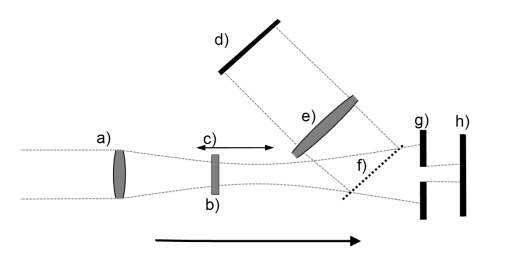
\includegraphics{img/zscan_sch.png}
 \caption{ The schematic diagram of the main measurement part of the z-scan experiment 
 \label{fig:zscan_sch}}
\end{figure}

\begin{figure}
 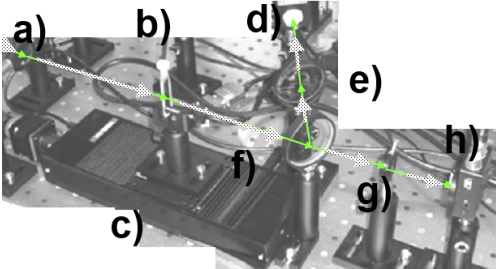
\includegraphics{img/zscan_diag.png}
 \caption{The photographic diagram of the main measurement part of the z-scan experiment 
 \label{fig:zscan_diag}}
\end{figure}

\subsubsection*{Legend for \ref{fig:zscan_sch} and \ref{fig:zscan_diag}}
Overview of the main measurement part of the z-scan set-up built at the Wroclaw University of Technology and being under usage
since summer 2010.
 
\begin{enumerate}[(a)]
  \item FOCUSING LENSE - A laser beam goes through focusing a lense.
  \item SAMPLE IN A QUEVETTE - Investigate sample is put into a silica quvette.
  \item DYNAMIC (MOBILE) STAGE - During experiment the sample changes its relative position from the lense
  \item DETECTOR 1 - Finally the beam reaches the ``Open-aperture'' detector  
  \item DEFOCUSING LENSE  - ``Open-aperture'' defocuing lense before detector
  \item BEAM SPLITTER - Laser beam is splitted to pass both through ''open-aperture'' and ''closed aperture'' with a beam splitter
  \item APERTURE - This is the aperture before the ``Closed-aperture'' detector
  \item DETECTOR 2 - Finally the beam reaches the ``Closed-aperture'' detector
\end{enumerate}

The inventor of the z-scan technique was the Dr. Mansoor Sheik-Bahae in 1989 \cite{bahae_sensitive} and since then many variants of this
technique have been deployed ``EZ-Scan", ``White Light z-scan", ``Excite-Probe z-scan" \cite{newport_application}. In a short
description - the z-scan technique uses a single laser beam, a mobile stage and two detectors - for the open and closed aperture.
Using physical model - we can relate the open-aperture results with the nonlinear absorption and the closed-aperture with the
nonlinear refraction index. The mobile stage moves the sample through the position focal point of the focusing lense. We therefore obtain
two diagrams - shown on \ref{fig:zscan_sch} and \ref{fig:zscan_diag}.


\begin{figure}
  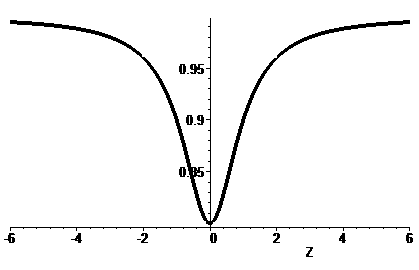
\includegraphics{img/oa_plot.png}
  \caption{A typical open-aperture transmittance $\Delta \,\mathrm{T}(Z)$ plot in a z-scan experiment, where \\ 
  $Z$ - the position of the stage/sample \\ 
  $0$ position - the focal point of focusing lense 
  \label{fig:oa_plot}}
\end{figure}


\begin{figure}
  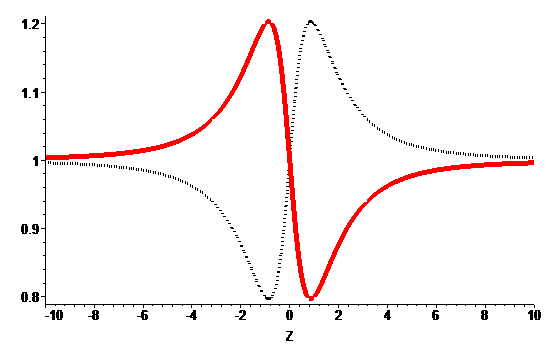
\includegraphics{img/ca_plot.png}
  \caption{A typical closed-aperture transmittance $\Delta \,\mathrm{T}(Z)$ plots in a z-scan experiment, where: \\  
    $Z$ - the position of the stage/sample, \\
    $0$ position - the focal point of focusing lense \\
    red (dashed) plot is for material with a positive (negative) refractive index
    \label{fig:ca_plot}}
\end{figure}

We must hereby stress that what we obtain with one z-scan measurement is only half a way to calculate one point in the nonlinear
spectrum plot - because a typical sample is held inside a silica cuvette and is soluted in some solution (for example chloroform or
toluen). So firstly we must measure the solution and an empty silica cuvette z-scan transmittance plots for each monochromatic
wavelength and after so - perform the z-scan experiment on the investigated sample. 

\textit{Description of the z-scan technique, description of the z-scan experiment built in Wroclaw, since summer 2010}

\subsection{Overview of the derivation} \label{chap:zscan_derivation}

\subsubsection*{Calculation of the nonlinear absorption coefficient:}

As shown of the \ref{fig:oa_plot} the open-aperture trasmittance can be described with the approximation equation:

\begin{equation}
  \Delta \,\mathrm{T}(Z)=\frac {\beta \,{I_{0}}\,(1 - e^{( - \alpha )}\,L)}{\alpha \,2\,\sqrt{2}\, \left(  \! 1 + \frac
  {Z^{2}}{(\frac {n\,\pi \,{w_{0}}\,2}{\lambda })^{2}} \!  \right) },
\end{equation}
 
where: 

\begin{tabular}{ r l }
   $\Delta \,\mathrm{T}(Z)$ & - normalized transmittance of the sample at $Z$ \\
   ${I_{0}}$ & - peak on-axis irradiance at focus \\
   $L$ & - sample length \\
   $\beta $ & - two-photon absorption coefficient \\
   $\alpha $ & - absorption coefficient \\
   $n$ & - index of refraction \\
   ${w_{0}}$ & - spot size at focus (radius at $\frac {1}{e^{2}}$) \\
   $\lambda $ & - laser wavelength \\
   $Z$ & - position of sample with respect to the focal position \\
\end{tabular}

We obtain the two-photon absorption coefficient while standard (f.e. least squares) fitting the measured open-aperture $\beta $ 
plot. This is of cource also not the complete truth, because with some advanced models we can also obtain other absorptive
nonlinearities. In a short description - the multiphoton absorption can be assumed when the closed-apperture peak is supressed, but
unfortunatelly the absorption saturation has got just the opposite effect. So the z-scan technique gives only the simple
information about the nonlinear absorption processes.

\subsubsection*{Calculation of the nonlinear refraction index:}

On the Figure \ref{fig:ca_plot} we can see the closed-aperture trasmittance plot with respect to the sample position Z. It has a
characteristic shape of peak trailing the valled or the valley trailing the peak if the ${n_{2}}$ sign is negative. What now
interest us is the difference between the peak and valley amplitude - we will call it $\Delta \,{T_{pv}}$. From this difference we
can calculate the on-axis peak nonlinear phase shift with sample at focus $\Delta \,{\Phi_{0}}$

\begin{equation} \label{eq:nlo_onaxisshift}
  \left| \! \,\Delta \,{\Phi_{0}}\, \!  \right| =\frac {\Delta \,{T_{pv}}}{0.407}\,(1 - S)^{0.27},
\end{equation}
where: 
\begin{tabular}{ r l}
  $S$ & - fraction of beam transmitted by the aperture \\
  $\Delta \,{T_{pv}}$ & - change in normalized transmittance between peak and valley. \\ 
\end{tabular}
Now we can estimate the refraction index from equation:

\begin{equation} \label{eq:nlo_estrefindex}
  {n_{2}}=\frac {\lambda \,\Delta \,{\Phi_{0}}}{2\,\pi \,{I_{0}}\,\frac {1 - e^{( - \alpha )}\,L}{\alpha }},
\end{equation}
where: 
\begin{tabular}{ r l}
  $\Delta \,{\Phi_{0}}$ & - on-axis peak nonlinear phase shift with sample at focus \\
  ${I_{0}}$  & - peak on-axis irradiance at focus \\
  $L$ & - sample length \\
  $\alpha $ & - absorption coefficient \\
  $\lambda $  & - laser wavelength \\
\end{tabular}

With data points collected for each wavelength we may obtain the full spectral plot for both nonlinear absorption coefficient and
nonlinear refraction index - due to the z-scan measurements.

\textit{Description how the gathered data is transformed into final chart. Some mathematical derivations.}

\subsection{Definition of the main problems} \label{chap:zscan_problems}

A typical z-scan experiment consists of the measurement routines with number more or less around 15-20 different wavelength. One
z-scan measurement usually takes between 5 to 10 minutes and together with:
\begin{enumerate}[(a)]
  \item long laser calibration process after each change of wavelength
  \item silica and empty-solution measurement
  \item measurement of a typical set of 10-20 measured cuvette samples it may take many days or even weeks to complete one
  measurement - so even such a simple routine is rather time-demanding. Therefore we are interested in optimizing the method, the
  physical theory understanding and the numerical precision, because the general error cumulates with the laser nonstability,
  method approximation error, fitting and numerical calculations error. 
\end{enumerate}

A typical plot containing the z-scan measurement for  the close aperture, open aperture and the laser reference is shown in the
Figure \ref{fig:zscan_both}

\begin{figure} 
  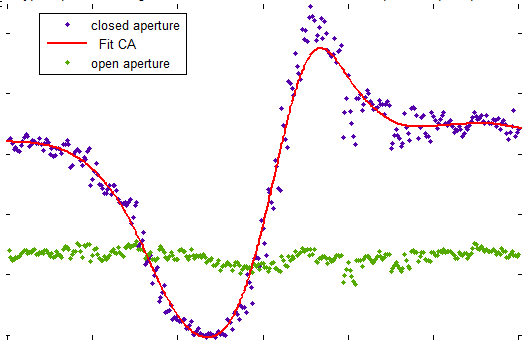
\includegraphics{img/zscan_both.png}
  \caption{A typical plot for both close and open aperture with respect to the sample position Z and with the fit splineline
  \label{fig:zscan_both}} 
\end{figure}

\textit{Discussion about the z-scan technique, its advantages and disadvantages for determination both real and imaginary part of
nonlinear susceptibility.}

\textbf{1. Is it not to short? Need to ask Prof. Samoc. Maybe we should also describe the ''White-Light or time-resolved ZScan''?}  

\section{Simpson and trapezoidal quadrature com\-bi\-ned \\ with cu\-bic in\-ter\-po\-la\-tion - HTRAN (solving)}
\label{chap:htran}

\subsection{Overview of the HTRAN} \label{chap:htran_overview}


We define the tabular-based function HTRAN and show its theoretical fundaments here. It has been implemented in MATLAB environment,
and its source code is avaiable in Appendix A.1 We shall start from the simplest possible numerical calculation of
integral - so the simpson and trapezoidal quadrature. The algorithm is based on report by I. J. Weinberg \cite{weinberg_hilbert} written for CDC
6600 supercomputer, but the difference is that it does not require the input function to be even. We first start from the
modification of the main Hilbert transform equation:

\begin{equation} \label{eq:htran_first_modification}
  \mathrm{HT}(\omega )=\frac {P\,\int_{ - \infty }^{\infty } \frac {\mathrm{R}(\Omega )}{\Omega  - \omega }\,d\Omega }{\pi } =
  {lim_{\varepsilon \rightarrow 0}} \left(  \! \int_{ - \infty }^{\omega  - \varepsilon }\frac {\mathrm{R}(\Omega )}{\Omega  -
  \omega }\,d\Omega  + \int_{\omega  + \varepsilon }^{\infty }\frac {\mathrm{R}(\Omega )}{\Omega  - \omega }\,d\Omega \!  \right),
\end{equation} 

as the integral uses the Cauchy Principal Value. 

\emptyline

We firstly observe, that:

\begin{equation} \label{eq:htran_observation0}
  \forall \omega : P\,\int_{ - \infty }^{\infty }\frac {1}{\Omega  - \omega }\,d\Omega =0
\end{equation}


Making any number of multiplications of \ref{eq:htran_observation0} does not change the fact it will equal zero - so we may obtain
a new form of the \ref{eq:htran_first_modification} integral:

\begin{equation} \label{eq:htran_newintegral}
  \mathrm{HT}(\omega )=\frac {P\,\int_{ - \infty }^{\infty }\frac {\mathrm{R}(\Omega ) - \mathrm{R}(\omega )}{\Omega - \omega
  }\,d\Omega }{\pi }
\end{equation}


As the proposed HTRAN method will take two arguments: \\
F[] - the tables of abscissas and R[] - the tabular ordinates \\
- we will assume that the function vanishes anywhere else - namely it equals zero:

\begin{equation} \label{eq:htran_vanishes}
  \forall ( \omega < F_{1} \wedge \omega < F_{N} ) : \mathrm{R}(\omega )=0  
\end{equation}

From \ref{eq:htran_newintegral} and \ref{eq:htran_vanishes} we obtain:

\begin{equation} \label{eq:htran_ht}
  \mathrm{HT}(\omega )=\frac {\int_{ - \infty }^{{F_{1}}} - \frac {\mathrm{R}(\omega )}{\Omega  - \omega }\,d\Omega  +
  \int_{{F_{1}}}^{{F_{N}}}\frac {\mathrm{R}(\Omega ) - \mathrm{R}(\omega )}{\Omega  - \omega }\,d\Omega  + \int_{{F_{N}}}^{\infty }
  - \frac {\mathrm{R}(\omega )}{\Omega  - \omega }\,d\Omega }{\pi }
\end{equation}

We shall also remember, that:

\begin{equation} \label{eq:htran_forallm}
  \forall M : \int_{ - \infty }^{\omega  - M}\frac {1}{\Omega  - \omega }\,d\Omega  + \int_{\omega + M}^{\infty }\frac {1}{\Omega 
  - \omega }\,d\Omega =0
\end{equation}

As $\omega  \in [{F_{1}}, \,{F_{N}}]$  we will now consider two conditions - that takes into account the position of  $\omega $ in
relation to ${F_{1}}$  and ${F_{N}}$ We have two posibilities:

\begin{subequations} \label{eq:htran_twoposibilities}
  \begin{equation}   \label{eq:htposs_closer}
    \omega - F_{1} < F_{N} - \omega \mbox{, which means that $\omega$ is placed closer to $F_{1}$ on the real axis }
  \end{equation}
  \begin{equation}   \label{eq:htposs_opposite}
    {F_{N}} - \omega \leq \omega  - {F_{1}} \mbox {, which is the opposite case and it is closer to ${F_{N}}$}
  \end{equation}
\end{subequations}


Each of these two cases leads to results obtained in (4.1.8a-b) we have:



\begin{subequations} \label{eq:htran_htresults}
  \begin{equation}   \label{eq:htran_htres1}
    \mathrm{HT}(\omega )= \left(  \! \frac {\int_{2\,\omega  - {F_{N}}}^{{F_{1}}} - \frac {\mathrm{R}(\omega )}{\Omega  - \omega
    }\,d\Omega  + \int_{{F_{1}}}^{{F_{N}}}\frac {\mathrm{R}(\Omega ) -  \mathrm{R}(\omega )}{\Omega  - \omega }\,d\Omega }{\pi
    }=\frac { - \mathrm{R}(\omega )\,\mathrm{ln}(\frac {{F_{1}} - \omega }{\omega  - {F_{N}}}) + \int_{{F_{1}}}^{{F_{N}}}\frac
    {\mathrm{R}( \Omega ) - \mathrm{R}(\omega )}{\Omega  - \omega }\,d\Omega }{\pi } \!  \right) 
  \end{equation}
  \begin{equation}   \label{eq:htran_htres2}
    \mathrm{HT}(\omega )= \left(  \! \frac {\int_{{F_{1}}}^{{F_{N}}}\frac {\mathrm{R}(\Omega ) - \mathrm{R}(\omega )}{\Omega  -
    \omega }\,d\Omega  + \int_{{F_{N}}}^{2\,\omega - {F_{1}}}\frac { - \mathrm{R}(\omega )}{\Omega  - \omega }\,d\Omega }{\pi
    }=\frac {\int_{{F_{1}}}^{{F_{N}}}\frac {\mathrm{R}(\Omega ) - \mathrm{R}(\omega )}{\Omega  - \omega }\,d\Omega  - \mathrm{R}(
    \omega )\,\mathrm{ln}(\frac {\omega - {F_{1}}}{{F_{N}} - \omega })}{\pi } \!  \right) 
  \end{equation}
\end{subequations}

And we can see that both the \ref{eq:htran_htresults} derivations lead to the same result:

\begin{equation} \label{eq:htran_sameresult}
  \mathrm{HT}(\omega ) = \frac { - \mathrm{R}(\omega )\, \mathrm{ln}( \frac {\omega  - {F_{1}}}{{F_{N}} - \omega }) +
 \int_{{F_{1}}}^{ {F_{N}}}\frac {\mathrm{R}(\Omega ) - \mathrm{R}(\omega )}{\Omega - \omega }\,d\Omega }{\pi }
\end{equation}

We also observe, that:

\begin{equation} \label{eq:htran_observations}
  \omega \,\ in\ \,[F_{1}, \,F_{N}] \Rightarrow (0 < \omega  - {F_{1}} \wedge 0 < {F_{N}} - \omega ) \Rightarrow (0 < \frac {\omega 
  - {F_{1}}}{{F_{N}} - \omega }) \Rightarrow \mathrm{ln}(\frac {\omega  - {F_{1}}}{{F_{N}} - \omega })
\end{equation}

What now interest us the most is the integral:

\begin{equation} \label{eq:htran_interestint} 
  \mathrm{Y}(\omega )=\int_{{F_{1}}}^{{F_{N}}}\frac {\mathrm{R}(\Omega ) - \mathrm{R}(\omega )}{\Omega  - \omega }\,d\Omega
\end{equation}


As the integrand in \ref{eq:htran_interestint} never explodes - we will calculate it numerically. We will need to prepare ourselves
to omit some difficulties - as when denominators equals zero. In algorithm we are preparing a new set of ${F_{x}}$ values, which
are just a simple midways of $\omega $ defined:

\begin{equation} \label{eq:htran_newpoints}
  {F_{x, \,k}}=\frac {{F_{k}} + {F_{k + 1}}}{2} \,\mbox{ for } \, k = 1\,\ldots\,{N - 1}
\end{equation} 

We will also need to obtain the values of a new ${R_{x}}$ table in this new ${\omega_{x}}$  values. We will do this by a simple
cubic interpolation:

\begin{subequations} \label{eq:htran_r3interp}
  \begin{equation}   \label{eq:hr3inp_first}
    {R_{x, \,1}} = \frac {3\,{R_{1}} + 6\,{R_{2}} - {R_{3}}}{8}
  \end{equation}
  \begin{equation}   \label{eq:hr3inp_next}
    {R_{x, \,k}} = \frac { - {R_{k - 1}} + 9\,{R_{k}} + 9\,{R_{k + 1}} - {R_{k + 2}}}{16} \,\mbox{ for } \, k = 2\,\ldots\,{N - 2}
  \end{equation}
  \begin{equation}   \label{eq:hr3inp_last}
    R_{x, \,{N-1}} = \frac { - {R_{N - 2}} + 6\,{R_{N - 1}} + 3\,{R_{N}}}{8}
  \end{equation}
\end{subequations}

By now the calculation of \ref{eq:htran_interestint} will be performed by a simple quadrature integration: 

\begin{equation} \label{eq:htran_simplequadrature}
  {Y_{x, \,i}}=\sum_{j=1}^{N}\,\frac {{h_{j}}\,({R_{j}} - {R_{x, \,i}})}{{F_{j}} - {F_{x, \,i}}} \,\mbox{ for } \, i =
  1\,\ldots\,{N - 1}
\end{equation}

To do such a integration we will hire both the trapezoidal rule and the Simpson's rule, depending on the evenness of N. If N is odd
only the Simpson's rule is used:

\begin{subequations} \label{eq:htran_nodd}
  \begin{equation}   \label{eq:hnodd_fnlast}
    {h_{1}} = {h_{N}} = \frac {{F_{2}} - {F_{1}}}{3} = \frac {\Delta \,F}{3}
  \end{equation}
  \begin{equation}   \label{eq:hnodd_even}
    {h_{j}} = \frac {4\,\Delta \,F}{3}  \,\mbox{ for } \,j=2, \,4\,\ldots\,{N - 1}
  \end{equation}
  \begin{equation}   \label{eq:hnodd_odd}
    {h_{j}} = \frac {2\,\Delta \,F}{3}  \,\mbox{ for } \,j=3, \,5\,\ldots\,{N - 2}
  \end{equation}
\end{subequations}

Where N is even, the last interval should be obtained using the trapezoidal rule:

\begin{subequations} \label{eq:htran_neven}
  \begin{equation}   \label{eq:hneven_first}
    {h_{1}} = \frac {\Delta \,F}{3} = \frac {{F_{2}} - {F_{1}}}{3}
  \end{equation}
  \begin{equation}   \label{eq:hneven_even}
    {h_{j}}=\frac {4\,\Delta \,F}{3}  \,\mbox{ for } \,j=2, \,4\,\ldots\,{N - 2}
  \end{equation}
  \begin{equation}   \label{eq:hneven_odd}
    {h_{j}}=\frac {2\,\Delta \,F}{3}  \,\mbox{ for } \,j=3, \,5\,\ldots\,{N - 3}
  \end{equation}
   \begin{equation}   \label{eq:hneven_prelast}
    {h_{N - 1}} = \frac {5\,\Delta \,F}{6}
  \end{equation}
   \begin{equation}   \label{eq:hneven_last}
    {h_{N}} = \frac {\Delta \,F}{2}
  \end{equation}
\end{subequations}

Next we calculate the Hilbert transform in the ${F_{x}}$ points:

\begin{equation} \label{eq:htran_htpoints}
  {HT_{x, \,i}}=\frac { - {R_{x, \,i}}\,\mathrm{ln}(\frac {{F_{x, \,i}} - {F_{x, \,1}}}{{F_{x, \,N - 1}} - {F_{x, \,i}}}) + {Y_{x, \,i}}}{\pi }
\end{equation}

Finally we need to undo the cubic interpolation. To do so, we perform the following calculations:

\begin{subequations} \label{eq:htran_undointp}
  \begin{equation}   \label{eq:htundo_first}
    {HT_{1}} = \frac {15\,{HT_{x, \,1}} - 10\,{HT_{x, \,2}} + 3\,{HT_{x, \,3}}}{8}
  \end{equation}
  \begin{equation}   \label{eq:htundo_second}
    {HT_{2}}=\frac {3\,{HT_{x, \,1}} + 6\,{HT_{x, \,2}} - 1\,{HT_{x, \,3}}}{8}
  \end{equation}
  \begin{equation}   \label{eq:htundo_next}
    {HT_{i}}=\frac { - {HT_{x, \,i - 1}} + 9\,{HT_{x, \,i}} + 9\,{HT_{x, \,i + 1}} - {\mathit{HT}_{x, \,i + 1}}}{16} \,\mbox{ for
    } \,i=3,\,4,\,\ldots\,{N - 2}
  \end{equation}
  \begin{equation}   \label{eq:htundo_prelast}
    {HT_{N - 1}}=\frac { - {HT_{x, \,N - 3}} + 6\,{HT_{x, \,N - 2}} + 3\,{HT_{x, \,N - 1}}}{8}
  \end{equation}
  \begin{equation}   \label{eq:htundo_last}
    {HT_{N}}=\frac {3\,{HT_{x, \,N - 3}} - 10\,{HT_{x, \,N - 2}} + 15\,{HT_{x, \,N - 1}}}{8}
  \end{equation}
\end{subequations}

In following chapters (or in Appendices) we will show the resultsobtained with this method.

\textit{Overview of the HTRAN method (originated by Winberg, with our modification for non-even functions)}

\subsection{HTRAN for simple linear model - results} \label{chap:htran_lin}

In the linear model we will assume that the susceptibility is calculated as the inverse Fourier transform of a decreasing,
sinusoidal and casual signal:
\begin{equation} \label{eq:htlin_resp}
  resp(t) = 1 - e^{( - t)}\,\mathrm{sin}(20\,t)\,\Theta (t) 
\end{equation}
The absorpance of the response signal - altogether with the transmittance signal should sum up to 1.

The plot of the equation \ref{eq:htlin_resp} is given on the figure \ref{fig:lin_plot}
\begin{figure}[H]
  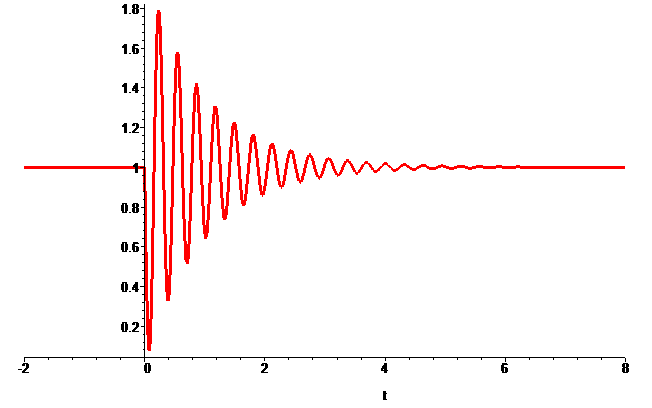
\includegraphics[width=150mm]{img/lin_plot.png}
  \caption{A typical linear response signal in time domain \label{fig:lin_plot}}
\end{figure}

First we need to calculate the Fourier transform of the signal from eq. \ref{eq:htlin_resp}:

\begin{equation} \label{eq:htlin_fresp}
  F[\mathrm{resp}(t)] = \chi (\omega )=\frac {2\,( - 10 - \pi \,\delta (\omega )\,\omega^{2} + 2\,i\,\pi \,\delta (\omega ) +
  401\,\pi \,\delta (\omega))}{(\omega \,i + 1 - 20\,i)\,(\omega \,i + 1 + 20\,i)} 
\end{equation}
\begin{alignat*}{1}
  \approx \frac{ -20}{(\omega \,i + 1 -20\,i)\,(\omega \,i + 1 + 20\,i)},
\end{alignat*}
where: $\delta (\omega )$ - Dirac delta function can be omitted from the numerical point of view.

\begin{figure} 
  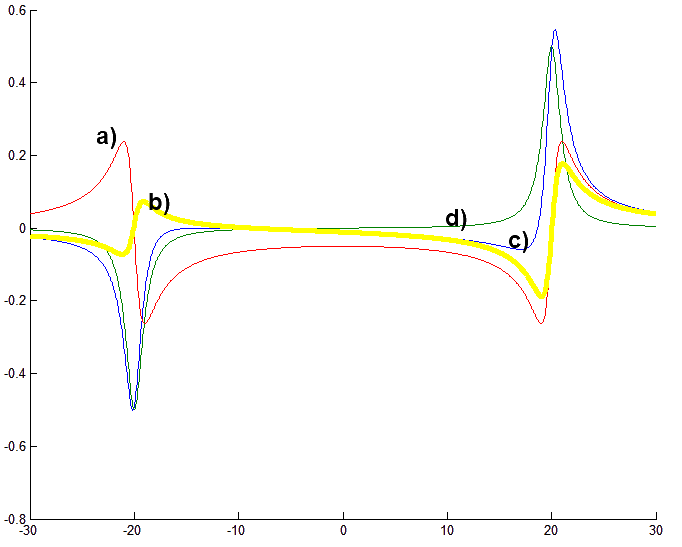
\includegraphics[width=150mm]{img/htran_lin.png}
  \caption{Results plotted together 
   a) The plot of the real part of $\chi (\omega )$ 
   b) absolute error plot (c-plot minus d-plot) 
   c) imaginary part of $\chi (\omega )$ obtained with the Hilbert transform of a-plot 
   d) part of $\chi (\omega )$ imaginary calculated analytically. \label{eq:htran_lin}
  }
\end{figure}

\footnotesize{\textit{Example cases for solving the Kramers-Kronig relations in linear model using HTRAN - with short conclusions}}

\subsection{HTRAN for simple nonlinear model - results} \label{chap:htran_nlo}

We get the equation for pump-and-probe susceptibility equation \ref{eq:pump_equation} and assume some values for the function
parameters:

\begin{equation} \label{eq:htran_fparameters}
  {\chi_{pp}}(\delta )=\frac {G\,{n_{0}}\,{\gamma_{ba}}\, \left( \! 1 - \frac {{\Omega_{1}}^{2}\,(\Delta - \delta  + I\,\eta
  )\,(\delta  + 2\,I\,\eta )}{(\Delta  - I\,\eta )\,((\delta  + I\,\theta )\,(\Delta  + \delta  + I\,\eta )\,(\delta - \Delta  +
  I\,\eta ) - {\Omega_{1}}^{2}\,(\delta  + I\,\eta ))\,2} \!  \right) }{\Delta  + \delta  + I\,\eta },
\end{equation}

where: $G = 1,\,{\gamma_{ba}} = -0.1,\, {n_{0}} = 1,\,\Delta = 1.3,\,\Delta = 1.3,\eta = 1, \theta = 1.4, \Omega_{1} = 4.3$

The results for such set of arbitrary parameters are shown on the Figure \ref{fig:htran_pnp_2d}.

\begin{figure}
  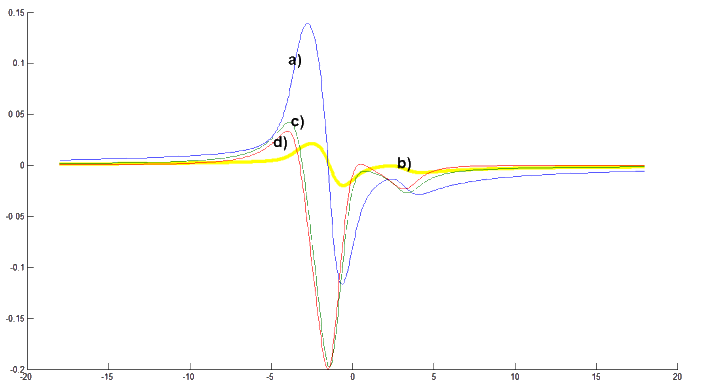
\includegraphics[width=150mm]{img/htran_pnp_2d.png}
  \caption{Result plotted together 
    a) The plot of the real part of $\chi_{pp} (\delta )$ 
    b) absolute error plot (c-plot minus d-plot) 
    c) imaginary part of $\chi_{pp} (\delta )$
    d) imaginary part of ${\chi_{pp}}(\delta )$ calculated analytically.
    \label{fig:htran_pnp_2d}}
\end{figure}

The resulted b-plot seems to be a not-so-bad introduction into the Hilbert transform evaluation, as we have only employed the
simple Simpson's rule. We would also like to perform the 3-Dimensional analysis of the assumed pump-probe susceptibility, so we
employ the (2.4.5a-b) equations for each frequency, which require performing two integrations (one, for each frequency-domain
argument). Unfortunatelly, only the obtained 3-Dimensial shapes are similary to the original ones, but the relative error is huge:

\begin{figure}
  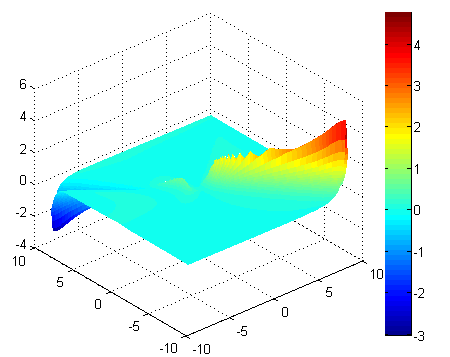
\includegraphics{img/htran_pnp_3derr.png}
  \caption{Combined relative error of 3-Dimensial calculations. The light-cyan color shows the area of error below 100\%, which is
  not very bad, but there are areas with error more above 100\%. \label{fig:htran_pnp_3derr}}
\end{figure}

Let's now perform the evaluation for the wave-mixing model as stated in the model described by \ref{eq:feff1_plus}. We expand this
equation to resolve the complex conjugate of D function and the resulting function is:

\begin{equation} \label{eq:htran_feffexp}
  {\chi_{mix}}(\delta ) = 
    \frac{2\,N\,{w_{0}}\,{\mu_{ba}}^{4}}{3\,\varepsilon_0\,h^{3}}( - \delta - \Delta - \frac {i}{{T_{2}}})\,(\delta +
    \frac{2\,i}{{T_{2}}})\,((\Delta + \frac {i}{{T_{2}}})\,\,(\Delta + \delta + \frac {i}{{T_{2}}})\,
\end{equation}
\begin{alignat*}{1}
  (\delta ^{3} - \frac
    {2\,i\,\delta ^{2}}{{T _{2}}} - \delta \,\Delta ^{2} - \frac {2\,i\,\delta }{{T_{1}}\,{T_{2}}} - \frac {\delta }{{T_{2}}^{2}} +
    \frac {\delta ^{2}}{{T_{1 }}} - \frac {\Delta ^{2}}{{T_{1}}} - \frac {1}{{T_{1}}\,{T_{2}}^{2}} - {\Omega_{2}}\,\delta  + \frac
    {{\Omega_{2}}\,i}{{T_{2}}}) )
\end{alignat*}

With such an complex function we obtain the following two and three dimensional results:
\begin{center}
  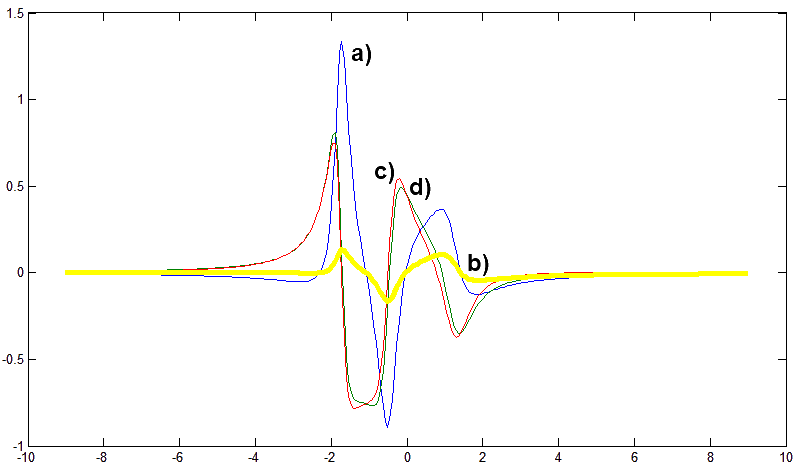
\includegraphics[width=150mm]{img/htran_fmix_2d.png}
  \captionof{figure}[htran_mix_2d]{Results plotted together
   a) The plot of the real part of ${\chi_{mix}}(\delta )$
   b) absolute error plot (c-plot minus d-plot)
   c) (red) imaginary part of  ${\chi_{mix}}(\delta )$
   d) (grey) imaginary part of ${\chi_{mix}}(\delta )$ calculated analytically.
   \label{fig:htran_mix_2d} 
   }
\end{center}

As the obtained 3-Dimensial shape looks very similar to those obtained analytically, the relative error still remains huge for some
areas:

\begin{center}
  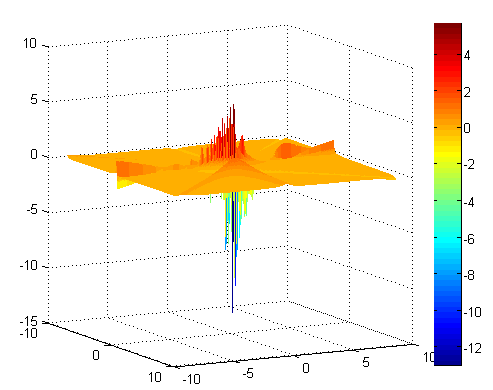
\includegraphics{img/htran_fmix_3derr.png}
  \captionof{figure}[htran_fmix_3derr]{Combined relative error for the real part of nonlinear susceptibility ${\chi_{mix}}(\delta
  )$ describing the wave-mixing process}
  \label{htran_fmix_3derr}
\end{center}

\textit{Example cases for solving the Kramers-Kronig relations in simple nonlinear model using HTRAN - with short conslusions.}

\subsection{HTRAN for simple quantum-perturbative model - results} \label{chap:htran_quantum}

We will use the models already prepared for both linear and second-order nonlinear susceptibilities defined
in the Chapter \ref{chap:problem_quantum}.

\begin{equation} \label{eq:htran_qpeq}
  \chi_{1, \,qp}(\omega ) = 
  \frac{N}{\varepsilon_0\,\hbar} \sum_{n=1}^{2}\,(\frac {{\mu_{1, \,n}}\,{\mu_{2, \,n}}}{{\Omega_{n}} - \omega -
  i\,{\gamma_{n}}} + \frac {{\mu_{2, \,n}}\,{\mu_{1, \,n}}}{{\Omega_{n}} + \omega + i\,{\gamma_{n}}}),
\end{equation}

where:

\begin{equation*}
  \mu = [[1, \,3], \,[ -1, \, -2]],\,\Omega =[3, \,16],\,\gamma =[1, \,2],\,N=5,\,\varepsilon_{0}=1, \,h= - 1
\end{equation*}



\begin{figure} 
  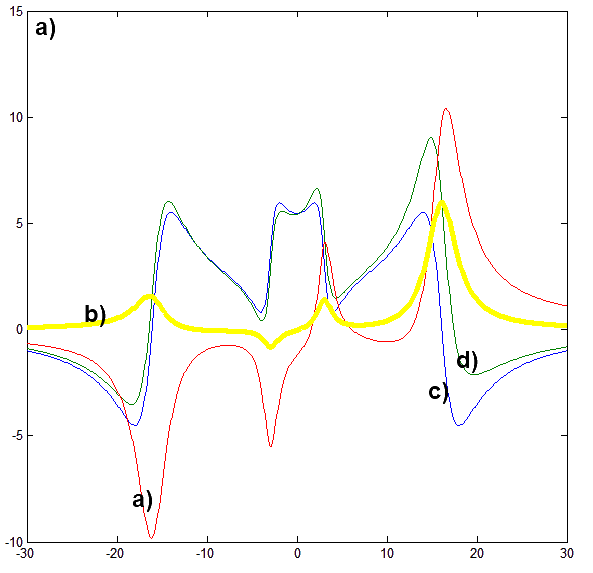
\includegraphics[width=70mm]{img/htran_qp_2da.png} 
  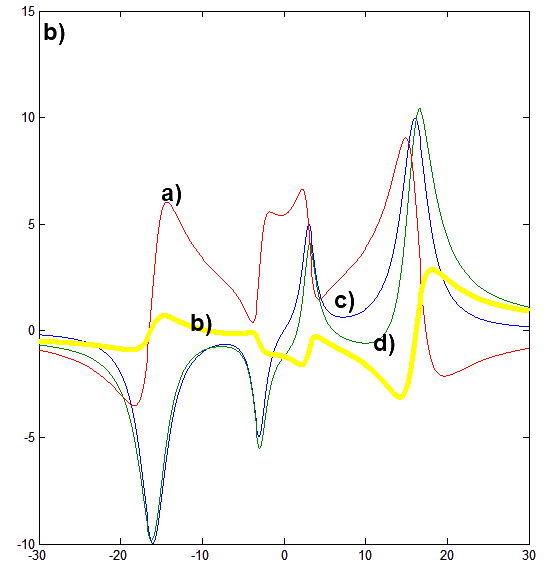
\includegraphics[width=70mm]{img/htran_qp_2db.png}  
  \caption{Results plotted together:
  a.a) The plot of the imag part of ${\chi_{1, \,qp}}(\delta )$ 
  a.b) absolute error plot (a.d-plot minus a.c-plot) 
  a.c) real part of ${\chi_{pp}}(\delta )$ calculated analytically
  a.d) real part of ${\chi_{1, \,qp}}(\delta )$ obtained with the Hilbert transform of a-plot
  b.a) The plot of the real part of ${\chi_{1, \,qp}}(\delta )$
  b.b) absolute error plot (b.d-plot minus b.c-plot)  
  b.c) imaginary part of ${\chi_{pp}}(\delta )$ calculated analytically 
  b.d) imaginary part of ${\chi_{1, \,qp}}(\delta )$ obtained with the Hilbert transform of a-plot 
  \label{htran_qp_2d}}
\end{figure}

\begin{equation}
  {\chi_{2, \,qp}}({\omega_{1}}, \,{\omega_{2}})=N \sum_{n=1}^{2} \sum_{m=1}^{2} \sum_{l=1}^{2}\,(
    \frac {{\mu_{l, \,n}}\,{\mu_{ nm}}\,{\mu_{ml}}}
      {({\Omega_{nl}} - \omega_1 - \omega_2 - i\,{\gamma_{nl}})\,({\Omega_{ml}} - \omega_1 - i\,{\gamma_{ml}})}
\end{equation}
\begin{alignat*}{1} 
  + \frac {{\mu_{l, \,n}}\,{\mu_{nm}}\,{\mu_{ml}}}
      {({\Omega_{nl}} - \omega_1 - \omega_1 - i\,{\gamma_{nl}})\,({\Omega_{ml}} - \omega_2 - i\,{\gamma_{ml}})} 
  + \frac {{\mu_{l, \,n}}\,{\mu_{nm}} \,{\mu_{ml}}}
      {({\Omega_{mn}} - \omega_1 - \omega_2 - i\,{\gamma_{mn}})\,({\Omega_{nl}} + \omega_2 + i\,{\gamma_{nl}})} 
+\\ + \frac {{\mu_{l, \,n}}\,{\mu_{nm}}\,{\mu_{ml}}}
      {({\Omega_{mn}} - \omega_1 - \omega_2 - i\,{\gamma_{mn}})\,({\Omega_{nl}} + \omega_2 + i\,{\gamma_{nl}})} 
  + \frac {{\mu_{l, \,n}}\,{\mu_{nm}}\,{\mu_{ml}}}
      {({\Omega_{nm}} + \omega_1 + \omega_2 + i\,{\gamma_{nm}})\,({\Omega_{ml}} - \omega_1 - i\,{\gamma_{ml}})} 
+\\ + \frac {{\mu_{l, \,n}}\,{\mu_{nm}}\,{\mu_{ml}}}
      {({\Omega_{nm}} + \omega_1 + \omega_2 + i\,{\gamma_{nm}})\,({\Omega_{ml}} - \omega_1 - i\,{\gamma_{ml}})} 
  + \frac {{\mu_{l, \,n}}\,{\mu_{nm}}\,{\mu_{ml}}}
      {({\Omega_{ml}} + \omega_1 + \omega_2 + i\,{\gamma_{ml}})\,({\Omega_{nl}} + \omega_1 + i\,{\gamma_{nl}})} 
+\\ + \frac {{\mu_{l, \,n}}\,{\mu_{nm}}\,{\mu_{ml}}}
      {({\Omega_{ml}} + \omega_1 + \omega_2 + i\,{\gamma_{ml}})\,({\Omega_{nl}} + \omega_2 + i\,{\gamma_{nl}})})  
      (2\,{ \varepsilon_{0}}\,h^{2})
\end{alignat*}

where: 
$\mu=[[1,\,3],\,[-1,\,-2]],\,\Omega=[[3,\,16],\,[4,\,12]],\,\gamma=[[1,\,2],\,[-1,\,3]],\,N=5,\,\varepsilon_{0}=1,\,h=-1$

 

\begin{figure}
  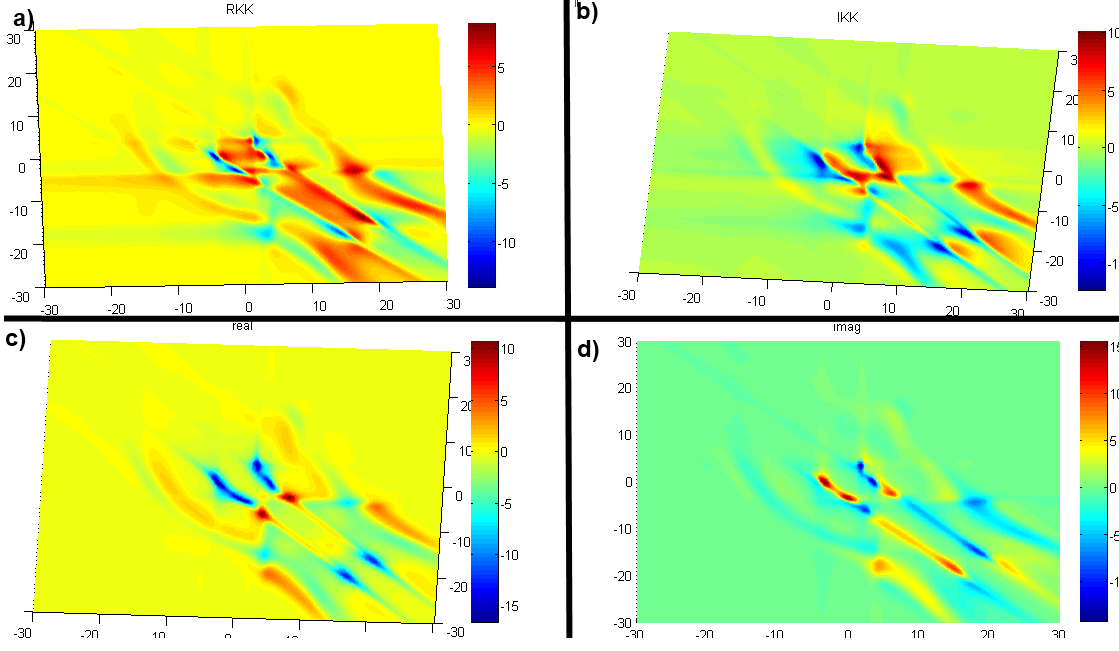
\includegraphics[width=150mm]{img/htran_qp_3d.png}
  \caption{Results of the HTRAN 3-Dimensional method plotted together.  
     a) - The calculated real part of ${\chi_{2, \,qp}}$ 
     b) The calculated imaginary part of ${\chi_{2, \,qp}}$ 
     c) The real part of nonlinear susceptibility ${\chi_{2, \,qp}}$ calculated analytically 
     d) The imaginary part of the nonlinear susceptibility ${\chi_{2, \,qp}}$
     \label{htran_qp_3d}}
\end{figure}

We can see, there is a similarity in obtained plots, but both the relative and absolute error do not satisfy us at all. Results
obtained with 2-Dimensional model were more satysfying.

Example cases for solving the Kramers-Kronig relations in simple quantum-perturbative model using HTRAN - with short conslusions.

\subsection{HTRAN for other models - results} \label{chap:htran_other}

Unfortunatelly the results obtained for the \ref{eq:dother_tpa} were far from accurate, so we will not show them for HTRAN method.

\textit{Example cases for solving the Kramers-Kronig relations for other models using HTRAN - with short conslusions.}

\section{Newton-Cotes quadrature (solving)} \label{chap:nc}
\subsection{Overview of the NC quadrature of arbitrary degree}  \label{chap:nc_quadrature}

Newton-Cotes formula for numerical integration is taken into consideration. We compare formula for an arbitrary degree - having in
our mind, that the choice between formulas of high and low degree must be undertaken with the awareness of numerical errors that
may arise. Newton-Cotes quadrature is a method for numerical integration with equispaced vertices. As we would like to integrate
function f = f(x) within the range $[a, b]$ we introduce the following calculations.

\begin{subequations} \label{eq:nc_parameters}
  \begin{equation}   \label{ncparms_x}
    {x_{n, \,k}}=a + \frac {(b - a)\,k}{n} \,\mbox{ for }\,k = 0, \,1,\,\ldots,\,n
  \end{equation}
  \begin{equation}   \label{eq:ncparms_omega}
    {\omega_{n}}(x) = (x - {x_{n, \,0}})(x - {x_{n, \,1}}),\,\ldots,\,(x - {x_{n, \,n}})
  \end{equation}
  \begin{equation}   \label{eq:ncparms_lambda}
    {\lambda_{n, \,k}}(x)=\frac {{\omega_{n}}(x)}{({\frac {\partial }{\partial x}}\,{\omega_{n}}({x_{n, \,k}}))\,(x - {x_{n,\,k}})}
    \, \mbox{ for}\, k = 0, \,1,\,\ldots,\,n
  \end{equation}
  \begin{equation}   \label{eq:ncparms_a}
    {A_{n, \,k}}=\int_{a}^{b}{\lambda_{n, \,k}}(x)\,dx = \frac {(b - a)\,( - 1)^{(n - k)}\,\int_{0}^{n}\prod_{j=0, \,j \neq
    k}^{n}\,(t - j)\,dt}{n\,k\mathrm{!}\,(n - k)\mathrm{!}}\, \mbox{ for }\,k = 0, \,1,\,\ldots,\,n
  \end{equation}  
\end{subequations} 

With such defined parameters the quadrature in sense of Newton-Cotes is defined as following:

\begin{equation} \label{eq:nc_mainequation}
   {NC_{n}}(f)={A_{n, \,k}}\, \left(  \! \sum_{k=0}^{n}\, (a + \frac {k\,(b - a)}{n}) \!  \right) 
\end{equation}

The numerical algorithm for the Newton-Cotes quadrature of an arbitrary degree has been prepared in Appendix A.2. It has been
modified to omit the singularity and to estimate the number of mini-steps needed to partition the integration range - see the
source code and comments. The function parameters are defined below:

\subsubsection*{Input arguments: }

\begin{tabular}{r l}
  fun & - the real-valued function we will like to integrate (function-handle), mandatory argument \\
  a & - integration starting point, mandatory argument \\
  b & - integration ending point, mandatory argument \\
  tol & - required tolerance, default value $10^{( - 5)}$ \\
  n & - degree of the Newton-Cotes quadrature, default value 8 \\
  cs & - how close (in absolute value) are we getting near the singularity, default value $10^{( - 2)}$ \\
  pts & - number of points to perform the discrete Hilbert transform, default value 200 \\
\end{tabular}


\subsubsection*{Output arguments:}
\begin{tabular}{r l}
  F & - an array of points, abscissas \\
  H & - calculated Hilbert transform values, ordinates \\
\end{tabular}

\textit{The description of the Newton-Cotes algorithm}

\subsection{NC for simple linear model - results} \label{chap:nc_lin}

As the prepared numeric method depends on many input parameter arguments, we have tried to perform the evaluation in many different
cases, some of those results are stated below. We are calculating the same model as in 4.2

\begin{equation} \label{eq:nc_algoritm}
  \chi (\omega ) \symbol{126} = \frac { - 20}{(\omega \,i + 1 - 20\,i)\,(\omega \,i + 1 + 20\,i)}
\end{equation} 

\begin{figure}
  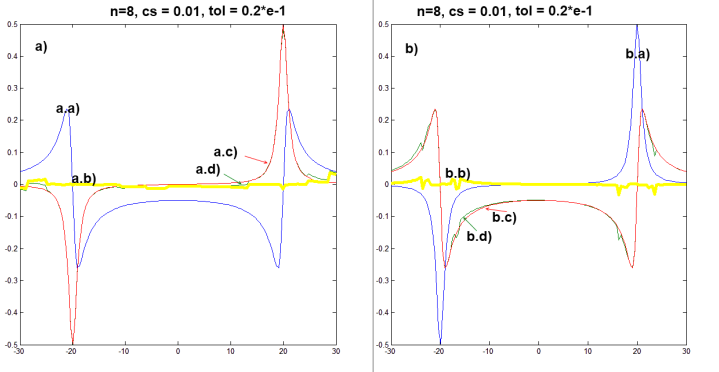
\includegraphics[width=150mm]{img/nc_lin1.png}
  \caption{Calcuations for parameters ($n=8, \,c s=\mbox{.1e-1}, \,tol=\mbox{.2e-1}$ 
     a.a) The plot of the real part of $\chi (\omega )$ 
     a.b) absolute error plot (a.d-plot minus a.c-plot) 
     a.c) imaginary part of $\chi (\omega )$ calculated analytically 
     a.d) imaginary part of $\chi (\omega )$ obtained with the Hilbert transform of a.a-plot, 
     b.a) The plot of the imaginary part of $\chi (\omega )$ 
     b.b) absolute error plot (b.d-plot minus b.c-plot) 
     b.c) real part of $\chi (\omega )$ calculated analytically 
     b.d) real part of $\chi (\omega )$ obtained with the Hilbert transform of b.a-plot 
     \label{fig:nc_lin1}
  }
\end{figure}

\begin{figure}
  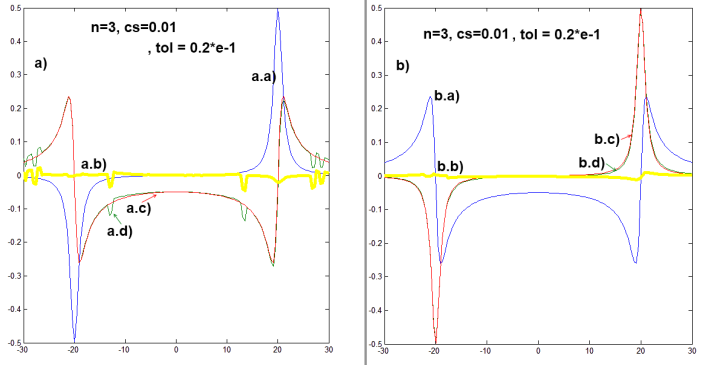
\includegraphics[width=150mm]{img/nc_lin2.png}
  \caption{
     Calcuations for parameters ($n=3, \,cs=\mbox{.1e-1}, \,tol=\mbox{.2e-1}$
     a.a) The plot of the imaginary part of $\chi (\omega )$
     a.b) absolute error plot (a.d-plot minus a.c-plot) 
     a.c) real part of $\chi (\omega )$ calculated analytically 
     a.d) real part of $\chi (\omega )$ obtained with the Hilbert transform of a.a-plot, 
     b.a) The plot of the real part of $\chi (\omega )$
     b.b) absolute error plot (b.d-plot minus b.c-plot)
     b.c) imaginary part of $\chi (\omega )$ calculated analytically 
     b.d) imaginary part of $\chi (\omega )$ obtained with the Hilbert transform of b.a-plot
     \label{fig:nc_lin2} 
  }
\end{figure}  

\begin{figure}
  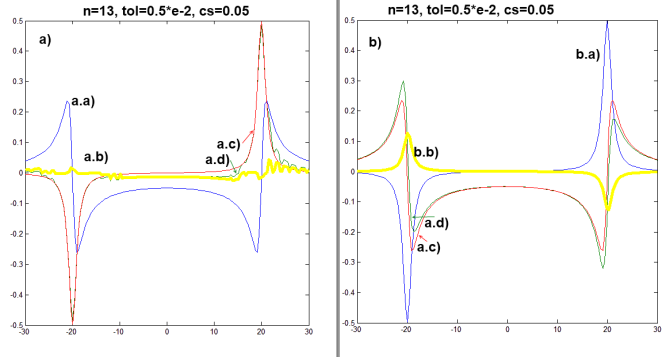
\includegraphics[width=150mm]{img/nc_lin3.png}
  \caption{
    Calcuations for parameters ($n=13, \,tol=\mbox{.5e-2}, \,cs=\mbox{.5e-1}$
    a.a) The plot of the real part of $\chi (\omega )$
    a.b) absolute error plot (a.d-plot minus a.c-plot) 
    a.c) imaginary part of $\chi (\omega )$ calculated analytically 
    a.d) imaginary part of $\chi (\omega )$ obtained with the Hilbert transform of a.a-plot, 
    b.a) The plot of the imaginary part of $\chi (\omega )$
    b.b) absolute error plot (b.d-plot minus b.c-plot) 
    b.c) real part of $\chi (\omega )$ calculated analytically 
    b.d) real part of $\chi (\omega )$ obtained with the Hilbert transform of b.a-plot
    \label{nc_lin3}     
  }
\end{figure}

\begin{figure}
  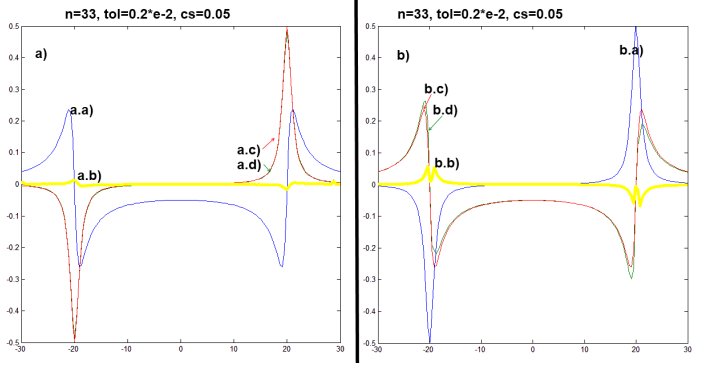
\includegraphics[width=150mm]{img/nc_lin4.png}
  \caption{Calcuations for parameters ($n=33, \,tol=\mbox{.2e-2}, \,cs=\mbox{.5e-1}$
    a.a) The plot of the real part of $\chi (\omega )$
    a.b) absolute error plot (a.d-plot minus a.c-plot) 
    a.c) imaginary part of $\chi (\omega )$ calculated analytically 
    a.d) imaginary part of $\chi (\omega )$ obtained with the Hilbert transform of a.a-plot,
    b.a) The plot of the imaginary part of $\chi (\omega )$
    b.b) absolute error plot (b.d-plot minus b.c-plot) 
    b.c) real part of $\chi (\omega )$ calculated analytically 
    b.d) real part of $\chi (\omega )$ obtained with the Hilbert transform of b.a-plot
    \label{nc_lin4} 
    }
\end{figure}

We cannot tell with hundred percent confidence which set of parameters will fit the best any given function and the user will need
to try many combinations before obtaining the final plot, but what we gave is the opportunity to set each one parameter manually,
which may lead to better results in the particular cases.

\textit{Example cases for solving the Kramers-Kronig relations in linear model using modified Newton-Cotes method - with short
conclusions.}

\subsection{NC for simple nonlinear model - results} \label{chap:nc_nlo}

We have performed calculations for the same both nonlinear pump-probe and wave-mixing model as in the chapter \ref{chap:htran_lin}.
Results for 1-dimension and 2-dimensions has been presented below:
\begin{equation} \label{eq:nc_chipp}
  {\chi_{pp}}(\delta ) = \frac {G\,{n_{0}}\,{\gamma_{ba}}}{\Delta  + \delta  + I\,\eta }\, \left(1 - \frac
  {{\Omega_{1}}^{2}\,(\Delta - \delta  + I\,\eta )\,(\delta  + 2\,I\,\eta )}{2\,(\Delta  - I\,\eta )\,((\delta  + I\,\theta
  )\,(\Delta  + \delta  + I\,\eta )\, (\delta  - \Delta  + I\,\eta ) - {\Omega_{1}}^{2}\,(\delta  + I\,\eta ))} \!  \right) 
\end{equation}
where: \\
$G=1, \gamma_{ba} = -0.1, n_{0} = 1, \Delta = 1.3, \eta = 1, \theta = 1.4, \Omega_{1}=4.3$ 
\begin{equation} \label{eq:nc_chimix}
  {\chi_{mix}}(\delta )= 6\,N\,{w_{0}}\,\varepsilon_0\,h^{3}\,{\mu_{\mathit{ba}}}^{4}
   \,( - \delta  - \Delta  - \frac {i}{{T_{2}}})
   \,(\delta  + \frac{2\,i}{{T_{2}}}) (\Delta  + \frac {i}{{T_{2}}})\,(\Delta  + \delta  + \frac
  {i}{{T_{2}}})\cdot
\end{equation}
\begin{alignat*}{1}
  \cdot	(\delta ^{3} - \frac {2\,i\,\delta ^{2}}{{T_{2}}} - \delta \,\Delta ^{2} - \frac {2\,i\,\delta }{{T_{1}}\,{T_{2}}}
  - \frac {\delta }{{T_{2}}^{2}} + \frac {\delta ^{2}}{{T_{1}}} - \frac {\Delta ^{2}}{{T_{1}}} - \frac {1}{{T_{1}}\,{T_{2}}^{2}} -
  {\Omega_{2}}\,\delta  + \frac {{\Omega_{2}}\,i}{{T_{2}}})
\end{alignat*}
where: $N=1, \,{w_{0}}=1, \,{\mu_{ba}}=1, \,{T_{1}}=1, \,{T_{2}}=2, \,{\Omega_{2}}=1, \,{\varepsilon_{0}}=1, \,h=1, \,\Delta =1$

\begin{figure} 
  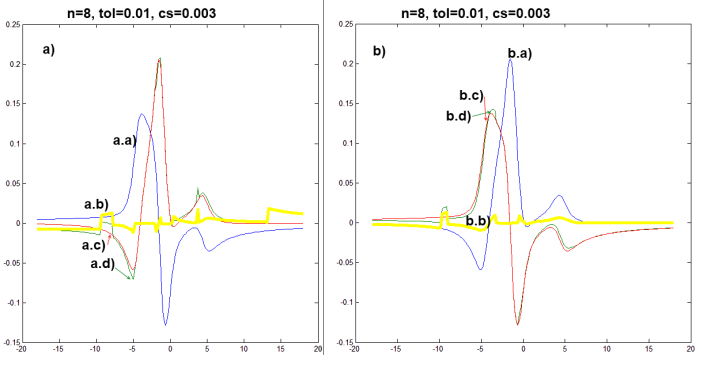
\includegraphics[width=150mm]{img/nc_fmix1.png}
  \caption{Calculations for parameters ($n=8, \,cs=\mbox{.3e-2}, \,tol=\mbox{.1e-1}$
     a.a) The plot of the real part of ${\chi_{pp}}(\delta )$
     a.b) absolute error plot (a.d-plot minus a.c-plot) 
     a.c) imaginary part of ${\chi_{pp}}(\delta )$ calculated analytically 
     a.d) imaginary part of ${\chi_{pp}}(\delta )$ obtained with the Hilbert transform of a.a-plot, 
     b.a) The plot of the imaginary part of ${\chi_{pp}}(\delta )$ 
     b.b) absolute error plot (b.d-plot minus b.c-plot) 
     b.c) real part of $\chi (\omega )$ calculated analytically 
     b.d) real part of ${\chi_{pp}}(\delta )$ obtained with the Hilbert transform of b.a-plot 
     \label{nc_fmix1}
     }
\end{figure}

\textit{Example cases for solving the Kramers-Kronig relations in simple nonlinear model using NC - with short conslusions}

\subsection{NC for simple quantum-perturbative model - results} \label{chap:nc_quantum}

\subsubsection*{Linear model - results:}

For the linear susceptibility we have used the model from the \ref{chap:problem_quantum}: 

\begin{equation} \label{nclin_chipp}
  {\chi_{1, \,qp}}(\omega ) = \frac { \left(  \! \sum_{n=1}^{2}\,(\frac {{\mu_{1, \,n}}\,{ \mu_{2, \,n}}}{{\Omega_{n}} - \omega  -
  i\,{\gamma_{n}}} + \frac {{\mu_{2, \,n}}\,{\mu_{1, \,n}}}{{\Omega_{n}} + \omega + i\,{\gamma_{n}}}) \!  \right) \,N}{\varepsilon
  0\,h}
\end{equation}

This time we have used the following parameters: \\
$\mu = [[3, \, - 0.5], \,[1.2, \,2.4]]$, \\ 
$\Omega =[ - 3, \,13]$, \\
$\gamma =[0.7, \,2.3]$, \\ 
$N=8$, \\ 
${\varepsilon_{0}}=1.4, \\
h= - 2.7$

Evaluation time of two plots given in the \ref{fig:nc_qp1} was 615 seconds.

\begin{figure}
  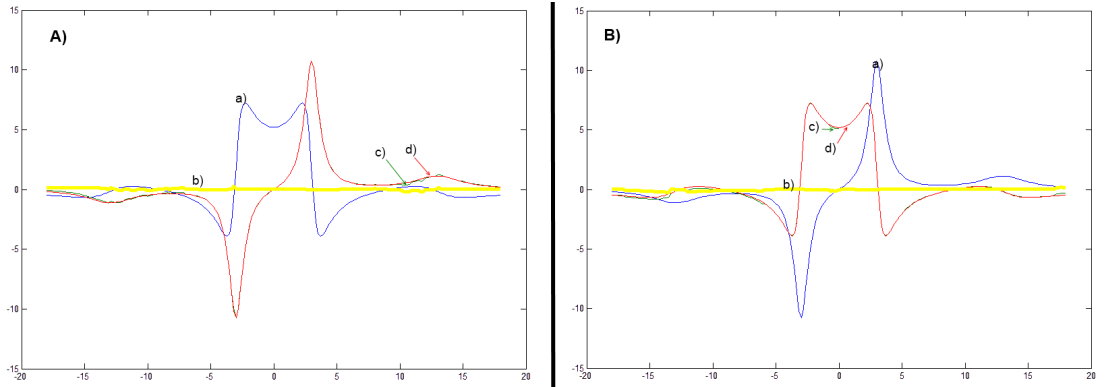
\includegraphics[width=150mm]{img/nc_qp1.png}
  \caption{Results plotted together 
    a.a) The plot of the imag part of ${\chi_{1, \,qp}}(\delta )$
    a.b) absolute error plot (d-plot minus c-plot) 
    a.c) real part of ${\chi_{1, \,qp}}(\delta )$ obtained with the Hilbert transform of a-plot 
    a.d) real part of ${\chi_{pp}}(\delta )$ calculated analytically 
    b.b) The plot of the real part of ${\chi_{1, \,qp}}(\delta )$ 
    b.b) absolute error plot (d-plot minus c-plot) 
    b.c) imaginary part of ${\chi_{1, \,qp}}(\delta )$ obtained with the Hilbert transform of a-plot 
    b.d) imaginary part of ${\chi_{pp}}(\delta )$ calculated analytically  
    \label{fig:nc_qp1}
  }
\end{figure}

\subsubsection*{Second-order model - results:}

For the second-order susceptibility we have used the model from the \ref{chap:problem_quantum}:

\begin{equation} \label{nclin_chipp2}
  \chi_{2, \,qp}({\omega_{1}}, \,{\omega_{2}})=N\,\sum_{n=1}^{2}\sum_{m=1}^{2}\sum_{l=1}^{2}\,
    (\frac {{\mu_{l,\,n}}\,{\mu_{nm}}\,{\mu_{ml}}}
      {({\Omega_{nl}} - \omega_1 - \omega_2 - i\,{\gamma_{nl}})\,({\Omega_{ml}} - \omega_1 - i\,{\gamma_{ml}})} +
\end{equation}
\begin{alignat*}{1}
  + \frac   {{\mu_{l, \,n}}\,{\mu_{nm}}\,{\mu_{ml}}}
      {({\Omega_{nl}} - \omega_1 - \omega_1 - i\,{\gamma_{nl}})\,({\Omega_{ml}} - \omega_2 - i\,{\gamma_{ml}})}
      \nonumber 
  + \frac   {{\mu_{l, \,n}}\,{\mu_{nm}}\,{\mu_{ml}}}
      {({\Omega_{mn}} - \omega_1 - \omega_2 - i\,{\gamma_{mn}})\,({\Omega_{nl}} + \omega_2 + i\,{\gamma_{nl}})}
      \nonumber 
+\\ + \frac{{\mu_{l, \,n }}\,{\mu_{nm}}\,{\mu_{ml}}} 
      {({\Omega_{mn}} - \omega_1 - \omega_2 - i\,{\gamma_{mn}})\,({\Omega_{nl}} + \omega_2 + i\,{\gamma_{nl}})} 
  + \frac   {{\mu_{l, \,n}}\,{\mu_{nm}}\,{\mu_{ml}}}
      {({\Omega_{nm}} + \omega_1 + \omega_2 + i\,{\gamma_{nm}})\,({\Omega_{ml}} - \omega_1 - i\,{\gamma_{ml}})}
      \nonumber
+\\ + \frac {{\mu_{l, \,n}}\,{\mu_{ nm}}\,{\mu_{ml}}}
      {({\Omega_{nm}} + \omega_1 + \omega_2 + i\,{\gamma_{nm}})\,({\Omega_{ml}} - \omega_1 - i\,{\gamma_{ml}})} 
  + \frac {{\mu_{l, \,n}}\,{\mu_{nm}}\,{\mu_{ml}}}
      {({\Omega_{ml}} + \omega_1 + \omega_2 + i\,{\gamma_{ml}})\,({\Omega_{nl}} + \omega_1 + i\,{\gamma_{nl}})}
      \nonumber 
+\\ + \frac {{\mu_{l, \,n}}\,{\mu_{nm}}\,{\mu_{ml}}}
      {({\Omega_{ml}} + \omega_1 + \omega_2 + i\,{\gamma_{ml}})\,({\Omega_{nl}} + \omega_2 + i\,{\gamma_{nl}})})  
      (2\,{\varepsilon_{0}}\,h^{2})
\end{alignat*}
where: \\
$\mu = \left| \begin{array}{cc} 
    1 & 3 \\ -1 & -2 
  \end{array} \right|,\, 
  \Omega = \left| \begin{array}{cc} 
    3 & 16 \\ 4 & 12 
  \end{array} \right|,\,
  \gamma = \left| \begin{array}{cc} 
  1 & 2 \\ -1 & 3
  \end{array} \right|,\, N=5,\, {\varepsilon_{0}}=1,\,h= - 1$

\emptyline

\textit{Example cases for solving the Kramers-Kronig relations in simple quantum-perturbative model using NC - with short
conslusions}

\subsection{NC for other models - results} \label{chap:nc_other}

Text and graphs here... 

\textit{Example cases for solving the Kramers-Kronig relations for other models using NC - with short conslusions.}

\section{Hilbert Clenshaw-Curtis iterations (solving)} \label{chap:hcc}

\subsection{Overview of the Hilbert Clenshaw-Curtis iterations} \label{chap:hcc_overview}

The adaptive and iterative algorithm for obtaining the Hilbert transform of a given regime of abscissas is presented. 

\subsubsection*{Clenshaw Curtis quadrature: }

The heart of the calculation is based on the typical Clenshaw-Curtis quadrature of function that has been expanded into a form of
Chebyshev polynomials. We define the quadrature problem as follows - for a given function f(x) find a value of the integral:

\begin{equation} \label{eq:cci_equation}
  CCI = \int_{ - 1}^{1}\mathrm{f}(x)\,dx
\end{equation}

The first step in solving this quadrature, after the idea of C.W. Clenshaw and A.R. Curtis \cite{clenshaw_method} is to do the
following change of variables:

\begin{subequations} \label{eq:cci_variables}
  \begin{equation} \label{eq:ccivars_x}
    x=\mathrm{cos}(\theta ) 
  \end{equation}
  \begin{equation} \label{eq:ccivars_cci}
    CCI = \int_{0}^{\pi }\mathrm{f}(\mathrm{cos}(\theta ))\,\mathrm{sin}( \theta )\,d\theta  
  \end{equation}
\end{subequations} 
 
By using the Discrete Cosine Transform of I-type, we can estimate the integral \ref{eq:ccivars_cci} with the following series:

\begin{subequations} \label{eq:cci_costrans}
  \begin{equation}   \label{eq:ccicos_main}
    \int_{0}^{\pi }\mathrm{f}(\mathrm{cos}(\theta ))\,\mathrm{sin}(\theta )\,d\theta \approx {a_{0}} +  \left( \! \sum_{k=1}^{\frac
    {N}{2} - 1}\,\frac {2\, {a_{2\,k}}}{1 - (2\,k)^{2}} \!  \right) + \frac {{a_{N}}}{1 - N ^{2}}  
  \end{equation}
  \begin{equation}   \label{eq:ccicos_parama}
    {a_{k}}=\frac {2\,\int_{0}^{\pi }f\,\mathrm{cos}(\theta )\, \mathrm{cos}(k\,\theta )\,d\theta }{\pi }  
  \end{equation}
\end{subequations}

Now we perform the simple approximation of \ref{eq:ccicos_parama} with:

\begin{equation} \label{eq:ccia_approx}
  {a_{k}} \approx \frac {2\, \left(  \! \frac {\mathrm{f}(1)}{2} + \frac {\mathrm{f}( - 1)\,( - 1)^{k}}{2} +  \left( \!
  \sum_{k=1}^{N - 1}\, \mathrm{f}(\mathrm{cos}(\frac {n\,\pi }{N}))\,\mathrm{cos}(\frac {n\,\pi \,k}{N}) \!  \right)  \!
  \right)}{N}
\end{equation}
 
And while in the \ref{eq:ccicos_main} we need only ${a_{2\,k}}$, the \ref{eq:ccia_approx} can be simplified:

\begin{equation} \label{eq:cci_a2k}
  {a_{2\,k}} \approx \frac {2\, \left(  \! \frac {\mathrm{f}(1) - \mathrm{f}( - 1)}{2} + \mathrm{f}(0)^{( - k)} +  \left(  \!
  \sum_{k=1}^{\frac {N}{2} - 1}\, \left(  \! \mathrm{f}(\mathrm{cos}(\frac {\pi \,n}{N}))+ \mathrm{f}( - \mathrm{cos}(\frac {\pi
  \,n}{N}))\,\mathrm{cos} \left(  \! \frac {n\,k\,\pi }{\frac {N}{2}} \!  \right)  \!  \right)  \!  \right)  \!  \right) }{N}  
\end{equation}

We can now simplify the \ref{eq:cci_a2k} using the matrix notation:

\begin{subequations} \label{eq:cci_matrix}
  \begin{equation}   \label{eq:ccimatrix_yn}
    {y_{n}}=\mathrm{f}(\mathrm{cos}(\frac {\pi \,n}{N}) + \mathrm{f}( - \mathrm{cos}(\frac {n\,\pi }{N})))  
  \end{equation}
  \begin{equation}   \label{eq:ccimatrix_dkn}
    {\mathrm{D}_{k, \,n}}=\frac {2\,\mathrm{cos} \left(  \! \frac {n\,k\,\pi }{\frac {N}{2}} \!  \right) \,{C_{k}}}{N}
    \qquad \mbox{ where: }\, {C_{k}} = 
    \begin{cases} 
      \frac {1}{2}\, & \mbox{ for }\,k = 0, N/2, \\ 
      1 & \mbox{ otherwise. } \\
    \end{cases}
  \end{equation}
\end{subequations}

We can observe, that both \ref{eq:cci_a2k} and \ref{eq:cci_matrix} describes the DCT-I transform. Now we use the statement, that
DCT-I is equivalent to a DFT of 2N - 2 real numbers with even symmetry. So we state:

\begin{subequations} \label{eq:cci_dft}
  \begin{equation}   \label{eq:ccidft_ym}
    {Y_{m}}={y_{2\,m}} \wedge {Y_{N - 1 - m}}={x_{2\,m + 1}}\,\mbox{ for }\, (m = 0, 1,\, \ldots,\,N/2-1)  
  \end{equation}
  \begin{equation}   \label{eq:ccidft_fy}
    FY = DFT(Y)
  \end{equation}
  \begin{equation}   \label{eq:ccidft_vectora}
    [a] = DCT-I(y) = \Re (e^{( - \frac {j\,n\,\pi }{2\,N})}\,FY)
  \end{equation}
\end{subequations} 

Now as we got the vector of a coefficients \ref{eq:ccidft_vectora} we can perform the final calculation by multiplying with vector
d:

\begin{equation} \label{eq:cci_vectord}
  {d_{0}} = 1, {d_{2\,k}}=\frac {2}{1 - (2\,k)^{2}}, {d_{N}}=\frac {1}{1 - N^{2}} 
\end{equation} 

And we get the final conslusion:

\begin{equation}
  \int_{ - 1}^{1}\mathrm{f}(x)\,dx=d^{T}\,[a]
\end{equation}

\subsubsection*{Hilbert transform using the Clenshaw-Curtis quadrature:}

While the Clenshaw-Curtis quadrature is defined for finite range $[-1,\,1]$, the Hilbert transform uses the definite and improper
integral over the range $[-\infty,\, \infty]$. What must now be done is to change the range of integrations without changing the
value of the Hilbert transform:

\begin{subequations} \label{eq:cci_range}
  \begin{equation}   \label{eq:ccirange_x}
    x = \frac {t}{1 - t^{2}}
  \end{equation}
  \begin{equation}   \label{eq:ccirange_hil}
    \textbf{Hil(f)(s)} = \frac {1\,\int_{ - \infty }^{\infty }\frac {\mathrm{f}(x)}{x - s}\,dx}{\pi } = \frac {1\,\int_{ -
    1}^{1}\frac {\mathrm{f}(\frac {t}{1 - t^{2}})\,(1 + t^{2})}{(t^{2} - 1)\,(t + s\,t^{2} - s)}\,dt}{\pi }
  \end{equation}
\end{subequations}
   
Our simple algorithm uses the implementation of Clenshaw-Curtis quadrature with the inner function:

\begin{equation} \label{eq:cci_innerfun} 
  g(t,s) = \frac {\mathrm{f}(\frac {t}{1 - t^{2}})\,(1 + t^{2})}{(t^{2} - 1)\,(t + s\,t^{2} - s)}
\end{equation}
 
In our implementation is adaptive - we compare two results for number of points N and 2*N - if the result is satisfactory, the loop
ends, if not - we continue with doubling the number of points in the Clenshaw-Curtis quadrature implementation - so the step and
tolerance must be selecter wisely.

\subsubsection*{Our implementation of the Hilbert Clenshaw-Curtis iterations:}

So far we have presented the overview of procedures responsible for evaluation of the Clenshaw-Curtis quadrature and the Hilbert
transform using the Clenshaw-Curtis quadrature in one point. But in the typical situation we have the whole vector of function
values for a given range of abscissas - so what is left - we perform the single-point Hilbert transform based on the
Clenshaw-Curtis quadrature for each given point. But to omit problems with singularities, we will add some post- and
precalculations - using the cubic interpolation. The whole procedure is now:

\textbf{INPUT:} \\ 
X, Y - given N-length abscissas and related ordinates

\emptyline

\textbf{PRE-CALCULATIONS:} \\
From N points of Y we calculate the cubic interpolation having N-1 inner points:

\begin{subequations} \label{eq:cci_cubicinterpolation}
  \begin{equation}   \label{eq:ccicinterp_first}
    {Yp_{1}}=\frac {3\,{Y_{1}} + 6\,{Y_{2}} - {Y_{3}}}{8}
  \end{equation}
  \begin{equation}   \label{eq:ccicinterp_next}
    {Yp_{k}}=\frac { - {Y_{k - 1}} + 9\,{Y_{k}} + 9\,{Y_{k + 1}} - {Y_{k + 2}}}{16}
  \end{equation}
  \begin{equation}   \label{eq:ccicinterp_last}
    {Yp_{N}}=\frac { - {Y_{N - 2}} + 6\,{Y_{N - 1}} + 3\,{Y_{N}}}{8}
  \end{equation}
\end{subequations}

\textbf{MAIN CALCULATIONS:} \\
With desired tolerance we calculate the N-1 values for each on of inner points:

\begin{equation} \label{eq:cci_approx}
  Hh_{k} \approx Hil(f)({Yp_{k}})
\end{equation}

\textbf{POST-CALCULATIONS:} \\
From N-1 points of Hh we calculate N points using the reverse cubic interpolation

\begin{subequations} \label{eq:cci_revcubicinterp}
  \begin{equation}   \label{eq:ccircinterp_first}
    {H_{1}}=\frac {15\,{Hh_{1}} - 10\,{Hh_{2}} + 3\,{Hh_{3}}}{8}
  \end{equation}
  \begin{equation}   \label{eq:ccircinterp_second}
    {H_{2}}=\frac {3\,{Hh_{1}} + 6\,{Hh_{2}} - {Hh_{3}}}{8}
  \end{equation}
  \begin{equation}   \label{eq:ccircinterp_next}
    {H_{k}}=\frac { - {Hh_{k - 1}} + 9\,{Hh_{k}} + 9\,{Hh_{k + 1}} - {Hh_{k + 2}}}{16}
  \end{equation}
  \begin{equation}   \label{eq:ccircinterp_prelast}
    {H_{N - 1}}=\frac { - {Hh_{N - 3}} + 6\,{Hh_{2}} - {Hh_{3}}}{8}
  \end{equation}
  \begin{equation}   \label{eq:ccircinterp_last}
    {H_{N}}=\frac {3\,{Hh_{N - 3}} - 10\,{Hh_{N - 2}} + 15\,{Hh_{N - 1}}}{8}
  \end{equation}
\end{subequations}

\textbf{OUTPUT:}
\begin{tabular}{r l}
  H & - N-length hilbert transform for given function values at X abscissas \\
\end{tabular}

\emptyline

The algorithm source has been presented in the Appendix A.3

\textit{Overview of the Clenshaw-Curtis iterations method}

\subsection{HCCI for simple linear model} \label{chap:hcc_lin}

Text and graphs here.... 

\textit{Example cases for solving the Kramers-Kronig relations in linear model using CCI - with short conclusions}

\subsection{HCCI for simple nonlinear model} \label{chap:hcc_nlo}

Text and graphs here.... 

\textit{Example cases for solving the Kramers-Kronig relations in simple nonlinear model using CCI - with short conslusions.}


\subsection{HCCI for simple quantum-perturbative model} \label{chap:hcc_quantum}
 
Text and graphs here.... 

\textit{Example cases for solving the Kramers-Kronig relations in simple quanum-perturbative model using CCI - with short
conslusions}

\subsection{HCCI for other models} \label{chap:hcc_other}

Text and graphs here.... 

\textit{Example cases for solving the Kramers-Kronig relations for other models using CCI - with short conslusions}

\section{Fast Hartley transform approach (solving)} \label{chap:hartley}

\subsection{Overview of the FTHA} \label{chap:hartley_overview}

The Fast Hartley Transform approach for the Hilbert transform is based on two efficient O (n log n) discrete Hartley transforms and
was well described by Soo-Chang Pei in \cite{chang_computation}. This approach is faster than another discrete Hilbert transform
based on two Fourier transorms, because the whole computation are carried using only real numbers, which is faster than Fourier computation carried
using time consuming complex numbers.

\subsubsection*{Discrete Hartley Transform}

For a given N-lenght vector X both the discrete Hartley transform and inverse discrete Hartley transform are defined as follows:

\begin{subequations} \label{eq:fhta_definition}
  \begin{equation}   \label{eq:fhtadef_dht}
    \mathrm{DHT}({X_{k}})=\sum_{n=0}^{N - 1}\,{X_{n}}\,(\mathrm{cos}(\frac {2\,\pi \,k\,n}{N}) + \mathrm{sin}(\frac {2\,\pi
    \,k\,n}{N}))
  \end{equation}
  \begin{equation}   \label{eq:fhtadef_idht}
    \mathrm{IDHT}({H_{k}})=\frac {\sum_{k=0}^{N - 1}\,{H_{n}}\,(\mathrm{cos}(\frac {2\,\pi \,k\,n}{N}) + \mathrm{sin}(\frac {2\,\pi
    \,k\,n}{N}))}{N}  
  \end{equation}
\end{subequations}

\subsubsection*{Hartley transform convolution theorem}

Now we will introduce the Hartley transform convolution theorem. We define the N-lenght vector x as convolution of two N-length
vectors ${x_{1}}$, ${x_{2}}$ as follows:

\begin{equation} \label{eq:hartley_convolution}
  {x_{n}}={x_{1, \,n}} = {x_{2, \,n}} = \sum_{k=0}^{N - 1}\,{x_{1, \,k}}\,{x_{2, \,n - k}} 
\end{equation}

For a given convolution, the following theorem is stated:

\begin{equation} \label{eq:hartley_theorem}
  \mathrm{DHT}({x_{n}})=\mathrm{DHT}({x_{1, \,k}})\,\mathrm{even}(\mathrm{DHT}({x_{2, \,k}})) + \mathrm{DHT}({x_{1, \, -
  k}})\,\mathrm{odd}(\mathrm{DHT}({h_{2, \,k}}))
\end{equation}

where: $\mathrm{DHT}({x_{2, \,k}})=\mathrm{even}(\mathrm{DHT}({x_{2, \,k}})) + \mathrm{odd}(\mathrm{DHT}({x_{2, \,k}}))$%

The proof of the Hartley transform convolution theorem can be found in \cite{chang_computation}. 

\subsubsection*{Relation between discrete Fourier and discrete Hilbert transform}

Now we will derive the discrete Fourier transform of the Hilbert transform for a given N-lenght vector x:

\begin{equation} \label{eq:hartley_dfttheorem}
  \mathrm{DFT}(\mathrm{DISCRETE\_HILBERT}({x_{k}}))=\mathrm{DFT}(\mathrm{h}(k))\,\mathrm{DFT}({x_{k}}) (-
  i)\,\mathrm{sgn}(k)\,\mathrm{DFT}({x_{k}})
\end{equation}

where: 

\begin{subequations} \label{eq:hartley_dfttparams}
  \begin{equation}   \label{eq:hdfttps_bigh}
    \mathrm{H}(k) = \mathrm{DFT}({h_{k}})
  \end{equation}
  \begin{equation}   \label{eq:hdfttps_smallh}
    {h_{k}}=\frac {1}{\pi \,k}\,\mbox{ discrete Hilbert kernel }  
  \end{equation}
\end{subequations} 

and also: 

\begin{subequations} \label{eq:hartley_defh}
  \begin{equation}   \label{eq:hdefh_fhalf}
    H(k) = i \,\mbox{ for }\, k=1, \,2,',\,\ldots,\,\frac {N}{2} - 1
  \end{equation}
  \begin{equation}   \label{eq:hdefh_middle}
    H(k) = 0\,\mbox{ for }\,  k=0, \,\frac {N}{2}
  \end{equation}
  \begin{equation}   \label{eq:hdefh_shalf}
    H(k) = -i\, \mbox{ for } \,k=\frac {N}{2} + 1, \,\frac {N}{2} + 2,\,\ldots,\,N - 1
  \end{equation}
\end{subequations}

\subsubsection*{Application of the discrete Hartley transform to calculate the discrete Hilbert transform:}

Using the Hartley transform convolution theorem \ref{eq:hartley_defh} for a given N-lenght vector x we obtain:

\begin{equation} \label{eq:hartley_fullconvolution}
  \mathrm{DHT}(\mathrm{DISCRETE\_HILBERT}({x_{k}}))=\mathrm{DHT}({x_{k}})\,\mathrm{even}(\mathrm{DHT}({h_{k}})) +
  \mathrm{DHT}({x_{- k}})\,\mathrm{odd}(\mathrm{DHT}({h_{k}}))
\end{equation} 

where: ${x_{ - k}}={x_{(N - k)\,\mathrm{mod}\,N}}$ (time reversal).

Now we should notice, that the discrete Hilbert transform kernel defined in \ref{eq:hdfttps_smallh} is an odd function, so its even
part equals zero. So \ref{eq:hartley_fullconvolution} simplifies now into a product of two separate Hartley transforms:

\begin{equation} \label{eq:hartley_simpleconvolution}
  \mathrm{DHT}(\mathrm{DISCRETE\_HILBERT}({x_{k}}))=\mathrm{DHT}({x_{ - k}})\,\mathrm{odd}(\mathrm{DHT}({h_{k}})) =
  \mathrm{DHT}({x_{- k}})\,\mathrm{DHT}({h_{k}})
\end{equation}

By \cite{chang_computation} the second transform is defined:

\begin{subequations} \label{eq:hartley_strans} 
  \begin{equation}   \label{eq:hstrans_fhalf}
    \mathrm{DHT}({h_{k}})=1\, \mbox{ for }\, k=1, \,2,\,\ldots,\,\frac {N}{2} - 1
  \end{equation}
  \begin{equation}   \label{eq:hstrans_middle}
    \mathrm{DHT}({h_{k}})=0\, \mbox{ for }\, k=0, \,\frac {N}{2}
  \end{equation}
  \begin{equation}   \label{eq:hstrans_shalf}
    \mathrm{DHT}({h_{k}})= - 1\, \mbox{ for }\, k=\frac {N}{2} + 1, \,\frac {N}{2} + 2 .. N - 1
  \end{equation}
\end{subequations}

If order to calculate the Hilbert of a given N-lenght vector x the last thing to do is apply the inverse discrete Hartley transform
on the very right side of \ref{eq:hartley_simpleconvolution} equation.

\subsubsection*{Fast Hartley Transform algorithm}

Ronald F. Ullmann has showed the fast algorithm for the discrete Hartley transform in \cite{ullmann_algorithm}. The important
assumption is that - as for the fast Fourier transform algorithm, the fast Hartley transform algorithm is defined for a K-length
vector x, where K is the power-of-two:

\begin{equation} \label{eq:ullmand_existp}
  \exists p\,\ \in\ \,N : K=2^{p}
\end{equation}


The \ref{eq:ullmand_existp} condition for the algorithm and the further possibilities to modify it are discussed further. We will
start with the very same thing as in the fast Fourier algorithm - we split the x vector into two smaller vectors:

\begin{subequations} \label{eq:hartley_smallervectors}
  \begin{equation}   \label{eq:hsvs_even}
    {x_{1, \,\frac {m}{2}}}={x_{m}}\, \mbox{ for }\, m=0, \,2,\,\ldots,\,N - 1
  \end{equation}
  \begin{equation}   \label{eq:hsvs_odd}
    {x_{2, \,\frac {m - 1}{2}}}={x_{m}}\, \mbox{ for }\, m=1, \,3,\,\ldots,\,N - 2
  \end{equation}
\end{subequations}

Taking into account the initial definition of the discrete Hartley transform \ref{eq:fhtadef_dht}, we obtain:

\begin{multline}  \label{eq:hartley_longdht}
 \mathrm{DHT}({x_{k}})= \left(  \! \sum_{n=0}^{\frac {N}{2} - 1}\,\mathrm{x}(2\,n)\,(\mathrm{cos}(\frac {2\,\pi \,k\,2\,n}{N}) +
 \mathrm{sin}(\frac {2\,\pi \,k\,2\,n}{N})) \! \right)  + \\
 \left(  \! \sum_{n=0}^{\frac {N}{2} - 1}\,\mathrm{x}(2\,n +
 1)\,(\mathrm{cos}(\frac {2\,\pi \,k\,(2\,n + 1)}{N}) + \mathrm{sin}(\frac {2\,\pi \,k\,(2\,n + 1)}{N})) \! \right)
\end{multline}

In \cite{ullmann_algorithm} the following ''shift rule'' for the discrete Hartley transform is stated :

\begin{equation} \label{eq:hartley_shiftrule}
  \mathrm{DHT}({x_{k + c}})=\mathrm{DHT}({x_{k}})\,\mathrm{cos}(c)
 + \mathrm{DHT}({x_{ - k}})\,\mathrm{sin}(c)
\end{equation}

If we apply the Hartley shift rule  \ref{eq:hartley_shiftrule} to the splitted equation in \ref{eq:hartley_longdht} we obtain:

\begin{multline} \label{eq:hartley_srapplied}
  \mathrm{DHT}({x_{k}})=\mathrm{DHT}({x_{1, \,k}}) + \mathrm{cos}(\frac {2\,\pi \,k}{N})\,\mathrm{DHT}({x_{2, \,k}}) +
  \mathrm{sin}(\frac {2\,\pi \,k}{N})\,\mathrm{DHT}({x_{2, \, - k}})\, \\
  \mbox{ for }\,k=0, \,1, \,3,\,\ldots,\frac {N}{2} - 1
\end{multline}

The rule \ref{eq:hartley_srapplied} can be applied only for the half of the possible k values ($k < \frac{N}{2}$). Now we will use
the periodic properties of the discrete Hartley transform kernel:

\begin{subequations} \label{eq:hartley_kernel}
  \begin{equation}   \label{eq:hkern_plus}
    \mathrm{cos}(\frac {2\,\pi \,k\,(n + N)}{N}) + \mathrm{sin}(\frac {2\,\pi \,k\,2\,(n + N)}{N})=\mathrm{cos}(\frac {2\,\pi
    \,k\,n}{N}) + \mathrm{sin}(\frac {2\,\pi \,k\,2\,n}{N})
  \end{equation}
  \begin{equation}   \label{eq:hkern_minus}
    \mathrm{cos} \left(  \! \frac {2\,\pi \,k\,(n + \frac {N}{2})}{N} \!  \right)  + \mathrm{sin} \left(  \! \frac {2\,\pi
    \,k\,2\,(n+ \frac {N}{2})}{N} \!  \right) = - (\mathrm{cos}(\frac {2\,\pi \,k\,n}{N}) + \mathrm{sin}(\frac {2\,\pi
    \,k\,2\,n}{N}))
  \end{equation}
\end{subequations}


The rule \ref{eq:hartley_srapplied} using the periodicity property from \ref{eq:hartley_kernel} can be now used for all k indices:

\begin{subequations} \label{eq:hartley_periodicity}
  \begin{equation}   \label{eq:hperiod_fhalf}
    \mathrm{DHT}({x_{k}})=\mathrm{DHT}({x_{1, \,k}}) + \mathrm{cos}(\frac {2\,\pi \,k}{N})\,\mathrm{DHT}({x_{2, \,k}}) +
    \mathrm{sin} (\frac {2\,\pi \,k}{N})\,\mathrm{DHT}({x_{2, \, - k}})
  \end{equation}
  
  for $\,k=0, \,1,\dotsc,\frac {N}{2} - 1$
  \begin{equation}   \label{eq:hperiod_shalf}
    \mathrm{DHT}({x_{k}})=\mathrm{DHT}({x_{1, \,k - \frac {N}{2}}}) - \mathrm{cos} \left(  \! \frac {2\,\pi \,(k - \frac
    {N}{2})}{N} \!  \right) \,\mathrm{DHT}({x_{2, \,k - \frac {N}{2}}}) - \mathrm{sin} \left(  \! \frac {2\,\pi \,(k - \frac
    {N}{2})}{N}  \! \right) \,\mathrm{DHT}({x_{2, \, - k + \frac {N}{2}}})
  \end{equation}
  
  for $\,k=\frac {N}{2}, \,\frac {N}{2} + 2,\dotsc,\,N - 1$ \\
\end{subequations} 
The remaining definition for the negative index, need to be explained:
\begin{equation} \label{eq:hartley_negindex}
  \mathrm{DHT}({v_{ - k}})=\mathrm{DHT}({v_{(N - k)\,\mathrm{mod}\,N}})
\end{equation}
Of course this is a typical divide'n'conquer approach, where the complexity is reduced from $\mathrm{O}(n^{2})\,$ to
$\,\mathrm{O}(n\,\mathrm{log}(n))$, very similar to the approach used in the Cooley-Tukey FFT algorithm \cite{Tukey_algorithm}.


\subsubsection*{Non-power-of-two case}

There are several approaches when calculating the fast Fourier transform for a non-power-of-two case length of the input x vector. 
One approach PFA is the Good-Thomas \cite{Good_interaction} / prime-factor algorithm for a vector length K defined:

\begin{equation}  \label{eq:hartley_goodk}
  K={K_{1}}\,{K_{2}},
\end{equation}

Where ${K_{1}}$ and ${K_{2}}$ are relatively prime numbers. Another approach was presented by Leo Bluestein, called also the chirp
z-transform algorithm is presented in \cite{bluestein_linear}. Another author, Georg Bruun, has invented the the approach based on
the recursive polynomial-factorization in \cite{bruun_ztransform}. Rader has prepared the special FFT algorithm expecially for
vectors of prime size in \cite{rader_dicrete}. But we will use the simplest possible approach - called the zero-padding. So in case
of input vector with the size of non-power-of-two, we add the suffix vector filled with vectors to fit the next possible
power-of-two size. In the worst case, there input vector size will be doubled, which has no influence on the asymptotic complexity,
which remains O(n log n). While the discrete signal analysis is the domain of scientists, we will end with conclusion stated by M.
Lamb in \cite{lamb_issues} that he is uncertain if zero padding has an influence on the spectral resolution, but in most cases it
has alittle influence on the results obtained in the discrete transforms.

The source code of the discrete Hilbert transform using both the fast Hartley transform and inverse fast Hartley transform has beed
presented in Appenxid A.4

\textit{Overview of the fast Hartley transorms, the algorithm is in O(n log n)}

\subsection{FTHA for simple linear model} \label{chap:hartley_lin}

Text and graphs here.... 

\textit{Example cases for solving the Kramers-Kronig relations in linear model using  - FTH with short conclusions.}

\subsection{FTHA for simple nonlinear model} \label{chap:hartley_nlo}

Text and graphs here.... 

\textit{Example cases for solving the Kramers-Kronig relations in simple nonlinear model using FTH - with short conslusions.}

\subsection{FTHA for simple quantum-perturbative model} \label{chap:hartley_quantum}

Text and graphs here.... 

\textit{Example cases for solving the Kramers-Kronig relations in simple quantum-perturbative model using FTH - with short
conslusions.}

\subsection{FTHA for other models} \label{chap:hartley_other}

More texts and graphics comes shortly.... 

\textit{Example cases for solving the Kramers-Kronig relations for other models using FTHA - with short conslusions.}

\section{Hermite-Hilbert transform (solving)} \label{chap:hermite}

\subsection{Overview of the HHT}  \label{chap:hermite_overview}

Hermite-Hilbert transform approach is based on the precalcution of already-known Hermite polynomials and Hermite base of orthogonal
functions. The algorithm is based on the master thesis of Mathias Johansson \cite{johansson_hilbert}.

\subsubsection*{Hermite polynomials and Hermite functions:}

Hermite polynomial of an arbitrary n degree is defined as follows:

\begin{equation} \label{eq:hermite_definition}
 {H_{n}}(x)=\frac {( - 1)^{n}\,e^{(x^{2})}\,d^{n}\,e^{( - x^{2})} }{dt^{n}}
\end{equation}

There is also an recursive equation for Hermite polynomials:

\begin{subequations} \label{eq:hermite_recursive}
  \begin{equation}   \label{eq:hrec_next}
    {H_{n}}(x)=2\,x\,{H_{n - 1}}(x) + 2\,(n - 1)\,{H_{n - 2}}(x)
  \end{equation}
  \begin{equation}   \label{eq:hrec_first}
    {H_{0}}(x)=1
  \end{equation}
\end{subequations}

Using the Hermite polynomial we would like to derive a set of orthogonal polynomials in $L^{2}$. Therefore we introduce the
weight function and the norm function:

\begin{subequations} \label{eq:hermite_weight}
  \begin{equation}   \label{eq:hwht_weight}
    \mathrm{w}(x)=e^{( - \frac {x^{2}}{2})}
  \end{equation}
  \begin{equation}   \label{eq:hwht_iter}
    {N_{n}}(x)=\sqrt{2^{n}\,n\mathrm{!}\,\sqrt{\pi }}
  \end{equation}
\end{subequations}

If we multiply the n-th Hermite polynomial with the weight function w(x) and divide it by the n-th norm function ${N_{n}}$ we
obtain a n-th orthogonal Hermite function:

\begin{equation} \label{eq:hermite_orthogonal}
  {\phi_{n}}(x)=\frac {\mathrm{w}(x)\,{H_{n}}(x)}{{N_{n}}(x)} = \frac {e^{( - \frac {x^{2}}{2})}\,{H_{n}}(x)}{\sqrt{2^{n}\,n
\mathrm{!}\,\sqrt{\pi }}}
\end{equation}

Based on the recursive equation in \ref{eq:hermite_recursive} we also obtain:


\begin{subequations} \label{eq:hermite_recresult}
  \begin{equation}   \label{eq:hrr_weight}
    {\phi_{n}}(x)=\sqrt{\frac {2\,x\,{\phi_{n - 1}}(x)}{n}} - (n - 1)\,\sqrt{\frac {{\phi_{n - 2}}(x)}{(n - 1)\,n}}
  \end{equation}
  \begin{equation}   \label{eq:hrr_iter}
    {\phi_{0}}(x)=\frac {e^{( - \frac {x^{2}}{2})}}{\pi ^{(\frac {1}{4})}}
  \end{equation}
\end{subequations}

\subsubsection*{Hilbert transform of Hermite functions:}


Johansson after polish mathematician Stefan L. Hahn \cite{hahn_hilbert} states that for any f(x) and
$\mathrm{HILBERT}(\mathrm{f}(x))$ belonging to ${L_{1}}$ we have:

\begin{equation} \label{eg:hermite_hproperty}
  \mathrm{HILBERT}(x\,\mathrm{f}(x))=x\,\mathrm{HILBERT}(\mathrm{F}(x)) - \frac {1\,\int_{ - \infty }^{\infty }\mathrm{f}(\tau
)\,d\tau }{\pi }
\end{equation}

The proof of the Theorem stated in \ref{eg:hermite_hproperty} is short:

\begin{equation} \label{eq:hermite_hpropproof}
  \mathrm{HILBERT}(x\,\mathrm{f}(x)) = \frac{1}{\pi }\,\dashint_{ -\infty }^{\infty } \frac {\tau \,\mathrm{f}(\tau )}{x - \tau
  }\,d\tau  = \frac {1}{\pi }\,\dashint_{ - \infty }^{\infty }\frac {(x - s)\,\mathrm{f}(x - s)}{s}\,ds,
\end{equation}
\begin{alignat*}{1}
  \mbox { where }\,s &= x - \tau = \frac{1}{\pi }\,\dashint_{ -\infty }^{\infty }\frac {x\,\mathrm{f}(x - s)}{s}\,ds -
  \frac{1}{\pi }\, \dashint_{ -\infty }^{\infty }\mathrm{f}(x - s)\,ds = \\
  &= x\,\mathrm{HILBERT}(\mathrm{f}(x)) - \frac {1}{\pi }\,\dashint_{ - \infty}^{\infty }\mathrm{f}(\tau )\,d\tau 
\end{alignat*}

From both equations \ref{eg:hermite_hproperty} and \ref{eq:hermite_recresult} we now obtain the important result:

\begin{subequations} \label{eq:hermite_impresult}
  \begin{equation}   \label{eq:hir_phinext}
    \mathrm{HILBERT}({\phi_{n}}(x))=\sqrt{\frac {2}{n}}\, \left( \! x\,{\phi_{n - 1}}(x) - \frac {1\,\int_{ - \infty
    }^{\infty}{\phi_{n - 1}}(\eta )\,d\eta }{\pi } \!  \right)  - (n - 1)\, \sqrt{\frac {1}{n\,(n - 1)}}\,{\phi_{n - 2}}(x)
  \end{equation}
  \begin{equation}   \label{eq:hir_phifirst}
    \mathrm{HILBERT}({\phi_{0}}(x))=2\,\sqrt{2}\,\pi ^{(\frac {1}{4})}\,\int_{0}^{\infty }e^{( - \frac {\omega
    ^{2}}{2})}\,\mathrm{sin}(\omega \,x)\,d\omega
  \end{equation}
\end{subequations}

\subsubsection*{Hilbert transform based on the Hermite functions:}

Now we can derive the Hilbert transform of an arbitrary function. We start with expanding f = f(x) into a series sum:

\begin{subequations} \label{eq:hermite_fexpand}
  \begin{equation}   \label{eq:hfe_f}
     \mathrm{f}(x)=\sum_{n=0}^{\infty }\,{a_{n}}\,{\phi_{n}}(x) 
  \end{equation}
  \begin{equation}   \label{eq:hfe_an}
     {a_{n}}(x)=\int_{ - \infty }^{\infty }\mathrm{f}(x)\,{\phi_{n}}(x)\,dx
  \end{equation}
\end{subequations}

For each function that has a limited series expansion at infinity we can provide an estimation used in further numerical algorithm:

\begin{subequations} \label{eq:hermite_estimate}
  \begin{equation}   \label{eq:hest_fapprox}
      f(x) \approx \sum_{n=0}^{N}\,{a_{n}}\,{\phi_{n}}(x
  \end{equation}
  \begin{equation}   \label{eq:hest_happrox}
     \mathrm{HILBERT}(\mathrm{f}(x)) \approx \sum_{n=0}^{N}\,{a_{n}}\,\mathrm{HILBERT}({\phi_{n}}(x))
  \end{equation}
\end{subequations}

\subsubsection*{Short description of the numerical algorithm:}

Taking a look on the \ref{eq:hermite_estimate} we can see, that the only difficulty is to calculate the ${a_{n}}$ coefficients,
while both the ${\phi_{n}}(x)$ and $\mathrm{HILBERT}({\phi_{n}}(x))$ can be precalculated once. The integral in
\ref{eq:hermite_fexpand} is now much easier because there is no singularity. The algorithm is given in Appendix A.5 and it
consists of three main parts:


\begin{tabular}{l}
  1. PRECALCULATION of Hermite function coefficients - done once using Maple Toolbox \\
  MAIN LOOP with: \\
  2. ESTIMATION OF ${a_{n}}$ COEFFICIENTS \\
  3. CALCULATION OF THE HILBERT TRANSFORM \ref{eq:hest_happrox} \\
\end{tabular}

\textit{Overview of the Hermite-Hilbert transorms and overview of the precalculation of the Hermite polynomials in a possibly short
time/memory}

\subsection{HHT for simple linear model} \label{chap:hermite_lin}

Text and graphs here.... 

\textit{Example cases for solving the Kramers-Kronig relations in linear model using  - HHT with short conclusions}

\subsection{HHT for simple nonlinear model} \label{chap:hermite_nlo}

Text and graphs here....

\textit{Example cases for solving the Kramers-Kronig relations in simple nonlinear model using HHT - with short conslusions}

\subsection{HHT for simple quantum-perturbative model} \label{chap:hermite_quantum}

Text and graphs here.... 

\textit{Example cases for solving the Kramers-Kronig relations in simple quantum-perturbative model using HHT - with short
conslusions}

\subsection{HHT for other models} \label{chap:hermite_other}

Text and graphs here.... 

\textit{Example cases for solving the Kramers-Kronig relations for other models using HHT - with short conslusions}

\section{Fourier-series (solving)} \label{chap:fourier}

\subsection{Overview of the Fouries-series based method}  \label{chap:fourier_overview}

The concept of the Hilbert transform evaluation based on the Fourier series also comes from the master thesis by Mathias Johansson
\cite{johansson_hilbert}. There is an important drawback in this approach - in general it should be applied to the periodical
functions, but we will further assume they have relatively long period. 

\subsubsection*{Fourier series:} 

Each periodical function can be decomposed into a infinite Fourier series. For a given periodic function f with a given period 2*P,
we will introduce the Fourier coefficients:

\begin{subequations} \label{eq:fourier_coeffs}
  \begin{equation}   \label{eq:fcoeffs_an}
    {a_{f, \,n}}=\int_{ - P}^{P}\mathrm{f}(x)\,\mathrm{cos}(n\,x)\, dx
  \end{equation}
  \begin{equation}   \label{eq:fcoeffs_bn}
    {b_{f, \,n}}=\int_{ - P}^{P}\mathrm{f}(x)\,\mathrm{sin}(n\,x)\, dx
  \end{equation}
\end{subequations}

Not getting deeply into harmonic analysis - we will assume that a series of partial sums:

\begin{equation} \label{eq:fourier_partialsums}
  {S_{f, \,N}}(x)=\frac {{a_{f, \,0}}}{2} + (\sum_{n=1}^{N}\,({a
_{f, \,n}}\,\mathrm{cos}(n\,x) + {b_{f, \,n}}\,\mathrm{sin}(n\,x)
))
\end{equation}

for a function $f\,\ \in \,{L_{2}}( - P, \,P)$ converges at almost every point to the f, which can be written as:

\begin{equation} \label{eq:fourier_canbewritten}
  \mbox{if }\,S = \{t : \lim_{N\rightarrow \infty }\,{S_{f, \,N}}(t) \neq \mathrm{f}(t) \} then |S| \leq {\aleph_{0}}
\end{equation}

\subsubsection*{Hilbert transform based on the Fourier series:}

After Johansson \cite{johansson_hilbert} we state that for any given function $f\,\ \textbf{in}\ \,{L_{2}}( - P, \,P)$ we can
calculate the Hilbert transform using the form of Fourier series for this function. All we need to do is to make a swap in the
\ref{eq:fourier_partialsums} equation - the ${a_{n}}$ coefficients should be swapped with ${b_{n}}$ coefficients.

\begin{equation} \label{eq:fourier_hilbert}
  HILBERT(f(x)) = \lim_{N\rightarrow \infty }\,\frac {{a_{f, \,0}}}{2} + (\sum_{ n=1}^{N}\,({b_{f, \,n}}\,\mathrm{cos}(n\,x)
+ {a_{f, \,n}}\, \mathrm{sin}(n\,x)))\,\mbox{ [at alm. every point x] }
\end{equation}

\subsubsection*{Algorithm overview:}

As mentioned before we will prepare the algorithm as for the periodic function, but we will try to imply that the period is much
longer than the area of interest. We would like to calculate the Hilbert transform for the both periodical and nonperiodical
function f. The first step is to calculate the properties of the input X interval, which is the region in which we are interested
of both input function f values and the values of its Hilbert transform. The second step is to calculate the Fourier coefficients
in a main loop. In the same loop we calculate the next partial sum values. The last step is to extract the inner interval from the
extended interval, to omit the numerical errors near the interval edges.

The full source code of this algorithm, has been presented in the appendix A.6.

\textit{The algorithm is ready, results will be generated - results are quite well for finite signals/spectras}

\subsection{Fouries-series for simple linear model} \label{chap:fourier_lin}

Text and graphs here.... 

\textit{Example cases for solving the Kramers-Kronig relations in linear model using Fourier-series - with short conclusions.}

\subsection{Fouries-series for simple nonlinear model} \label{chap:fourier_nlo}

Text and graphs here.... 

\textit{Example cases for solving the Kramers-Kronig relations in simple nonlinear model using Fourier-series - with short
conslusions}

\subsection{Fouries-series for simple quantum-perturbative model} \label{chap:fourier_quantum}

Text and graphs here.... 

\textit{Example cases for solving the Kramers-Kronig relations in simple quantum-perturbative model using Fourier-series - with
short conslusions}

\subsection{Fouries-series for other models} \label{chap:fourier_other}

Text and graphs here.... 

\textit{Example cases for solving the Kramers-Kronig relations for other models using Fourier-series - with short conslusions}

\section{MATLAB ® out-of-the-box functions (solving)} \label{chap:matlab}

\subsection{Overview of the MATLAB ® interior functions} \label{chap:matlab_overview}

Why not take into consideration the already built-in numerical methods from MATLAB? We compare the results obtained with: 
\begin{tabular}{r l}
  - quadgk() - adaptive Gauss-Kronrod quadrature; \\
  - hilbert() - fast Hilbert transform based on both FFT and IFFT. \\
\end{tabular}

\subsubsection*{Adaptive Gauss-Kronrod quadrature - theory:}

The source code of the adaptive Gauss-Kronrod quadrature has been published in the popular Fortran 77 numerical integration
QUADPACK library and has been also translated into the MATLAB core language. It is also based on the ''quadva'' routine decribed by
Lawrence F. Shampine in \cite{shampine_vectorized}. The foundamental idea of this numerical integration algorithm is the nested
quadrature rule - the more accurate quatradure approximation is calculated from the less accurate one. The algorithm is adaptive
and the error estimation is based on the (G-K7,15) pair of the quadrature rules - less and more accurate - the 7-point Gauss rule
and the 15-point Kronrod rule with a share nodes. For more information about the theory beneath this algorithm - please read D.
Calvetti et al \cite{calvetti_computation} or the \ref{chap:nc_other} from the book by David Kahaner \cite{kahaner_numerical}.

\textit{Short overview on the Gauss-Kronrod quadrature theory}

\subsubsection*{Adaptive Gauss-Kronrod quadrature - short tutorial:}

With the given theory the MATLAB implementation of the Gauss-Kronrod quadrature has been prepared to work as flexible as possible.
The user is able to cope with given parameters. Three of them are important for us: \\
A. 'Waypoints' - the most important parameter when performing the numerical integration with a singularity. As the Hilbert
transform already has the singularity by definition, we will need to properly define the waypoint for each calculation;

B. '''AbsTol' and ''RelTol'' - the absolute and the relative error tolerance, to control the calculation time and its accuracy. The
short tutorial MATLAB m-file with examples and more practical explanation has been presented in the Appendix B.1.

\textit{The short tutorial overview on the MATLAB® quadgk() function usage}

\subsubsection*{Fast Hilbert transform routine - theory:}

The discrete Hilbert transform (DHT) is given by definition after \cite{kak_multilayeredarray} - for a given n-length X vector:

\begin{equation} \label{eq:matlab_fhttheroy}
  \mathrm{DHT}({X_{k}})=\frac { \left(  \! \sum_{s=0}^{n - 1}\,{X _{s}}\,(1 - ( - 1)^{(k - s)})\,\mathrm{cot}(\frac {\pi \,(k - s)
}{n}) \!  \right) \,1}{n}
\end{equation}

The other definition by \cite{calvetti_computation} uses the convolution:

\begin{subequations} \label{eq:matlab_convolution}
  \begin{equation}   \label{eq:mconv_dht}
    \mathrm{DHT}({X_{k}})  = X[] * h[] = \sum_{s=0}^{n - 1}\,{h_{k - s}}\,{X_{s}}
  \end{equation}
  \begin{equation}   \label{eq:mconv_hk}
    {h_{k}}=\frac { \left(  \! \mathrm{cot}(\frac {\pi \,k}{n}) - \frac {\mathrm{cos}(\pi \,k)}{\mathrm{sin}(\frac {\pi \,k}{n})}\!
      \right) \,1}{n}
  \end{equation}
\end{subequations}

The important issue is that the DHT is closely related to the discrete Fourier transform (DFT). For a given n-length X vector in
order to evaluate the DHT(X) we can hire the DFT routine. To start, we must remember that in the continous case:

\begin{equation} \label{eq:matlab_issue}
  \mathrm{FOURIER}(\mathrm{HILBERT}({X_{k}}))=( - i\,\mathrm{sgn}( \frac {n}{2} - k)\,\mathrm{sgn}(k))\,\mathrm{FOURIER}({X_{k}})
\end{equation}

where:

\begin{equation} \label{eq:matlab_kernel}
   - i\,\mathrm{sgn}(\frac {n}{2} - k)\,\mathrm{sgn}(k)=\mathrm{FOURIER}(\frac {1}{\pi \,k})
\end{equation}

Therefore in the discrete case we find the similar equation to \ref{eq:matlab_issue} relating the DHT and DFT:

\begin{equation} \label{eq:matlab_reldhtdft}
  \mathrm{DFT}(\mathrm{DHT}({X_{k}}))=( - i)\,\mathrm{sgn}(\frac {n}{2} - k)\,\mathrm{sgn}(k)\,\mathrm{DFT}({X_{k}})
\end{equation}

From the \ref{eq:matlab_reldhtdft} we can see, that it is quite easy to operate within the Fourier/frequency domain - because the
quite complicate convolution is transformed to a simple algebraic operations. Also - if we have the quick algorithm to perform both
the DFT and inverse-DFT - for example with the fast Fourier transform (FFT) and the inverse fast Fourier transform (IFFT) - the DHT
operation will be calculated as follows:

\begin{equation} \label{eq:matlab_fulldhthdf}
  \mathrm{DHT}({X_{k}})=\mathrm{IDFT}(( - i)\,\mathrm{sgn}(\frac {n}{2} - k)\,\mathrm{sgn}(k)\,\mathrm{DFT}({X_{k}}))
\end{equation}

\textit{The foundametals of the discrete Hilbert transform and its relation with the discrete Fourier transform}

\subsubsection*{Fast Hilbert transform routine - short tutorial:}

While the hired DFT and IDFT routines are evaluated in complex domain, for a given input n-length X vector we have that:

\begin{equation} \label{eq:matlab_implication}
  \mathrm{hilbert}(X) \Rightarrow X + i\,\mathrm{DHT}(X)
\end{equation}

In order to obtain the final result we need to take the imaginary part of the \textit{MATLAB® hilbert() }function output. The other
important issue is that the \textit{MATLAB® hilbert()} function has one optional parameter called N - to computer the N-point Hilbert transform. If the input vector X is too short, it will be padded with zeros, otherwise it will be truncated.

The short tutorial MATLAB m-file with examples and more practical explanation has been presented in the Appendix B.2

\textit{The short tutorial overview on the MATLAB® hilbert() function usage}

\textit{Overview of the method using MATLAB ® interior functions}

\subsection{MIF for simple linear model} \label{chap:matlab_lin}

Text and graphs here.... 

\textit{Example cases for solving the Kramers-Kronig relations in linear model using MIF - with short conclusions}

\subsection{MIF for simple nonlinear model} \label{chap:matlab_nlo}
Text and graphs here.... 

\textit{Example cases for solving the Kramers-Kronig relations in simple nonlinear model using MIF - with short conslusions}

\subsection{MIF for simple quantum-perturbative model} \label{chap:matlab_quantum}

Text and graphs here.... 

\textit{Example cases for solving the Kramers-Kronig relations in simple quantum-perturbative model using MIF - with short
conslusions}

\subsection{MIF for other models} \label{chap:matlab_other}

Text and graphs here.... 

\textit{Example cases for solving the Kramers-Kronig relations for other models using MIF - with short conslusions}

\section{General comparison of used numerical methods (understanding)} \label{chap:comparison}

\subsection*{HTRAN conlusions:} \label{chap:comparison_htran}

HTRAN method is fast (it employes the full-vector calculation at once) but for most cases is very inaccurate 

\subsection*{Newton-Cotes method conlusions:} \label{chap:comparison_nc}

Newton-Cotes method is extremely time demanding (it takes more than 10 minutes for one model even if we require small tolerance),
because it employes the new quadrature routine for each calculation point, as it is the method close to analitycal (without any
full-vector manipulations). For the advanced - multi-dimensionoal

\subsubsection*{Comparison:}

We can divide methods in two groups.  In the first group numerical methods works on the full vectors and are
not so accurate, but very usefull for the multidimensional calculations.

In the second group numerical methods works on points, these methods are more accurate and better for one-dimensional evaluation,
but may be sometimes time demanding.

\textit{Nice charts of numerical comparisons here :)}

\section{Conclusion (understanding)} \label{chap:conclusion}

\subsection{Model conclusion} \label{chap:conclusion_model}

We have presented both the linear and nonlinear model with comments that arise from the literature. The main question remains -
what is the true and valid model for describing the interation of finite amount of photons with chemical molecules

\emptyline

1. Kramers-Kronig relations in general are false - because they assume that imaginary part must be an odd function and the real
part must be an even function. We state, that only in general case - we can talk about the conjugate integral pairs, so the real
and imaginary part are connected with Hilbert (not with the K-K) transform.

\emptyline

2. Only linear model - we can assume the even/odd properties being 100\% sure.

\emptyline

3. The Lorentz/Gauss discussion

\emptyline

4. Response discussion, relaxation time, extended causality principle, multistep multiphoton absorption

\textit{Final discussion about the used models}

\subsection{Numerical conclusion} \label{chap:conclusion_numerical}

We have presented several methods and the comparison of their accuracy, convergency and speed. Which method is the best and why?

\emptyline

1. The FFT-based algorithms cannot be used as-they-are, we need to
estimate of the left and right


\emptyline

2. 


\textit{Final discussion about the used numerical methods and their accuracy}

\subsection{Z-scan technique conclusion} \label{chap:conclusion_zscan}

The Z-scan experiment was the most important motivation for this thesis to be written. It is of course one of many experimental
setups in nonlinear optics - but the questions are: \\
- how both the experimental and numerical accuracy influence on the final results \\
- how to avoid this problems in the z-scan experiment? \\
\emptyline

1. We need to correct the error bars

2. We should try to somehow geometrically orient all investigated molecules within a sample (some outer electromagnetic field) to
check any susceptibility tensor element - not only to make the so-called averaging, which may lead to not a complete perspective

3. We should correct the data collection in relation to laser instability.

4. We should establish an numericaly proper algorithm to some advanced fitting with valid models in complex domain.

5. Maybe it will be possible to combine the Z-scan technique with the pump-and-probe approach?

\textit{Final discussion for the building better z-scan experiment (Z-scan 2.0 ? :))}

\subsection{General conclusion} \label{chap:conclusion_general}

1. This thesis in only an introduction into an important, but hard interdisciplinary problem concerning the investigation of light
and matter interaction in area of nonlinear optics. 

2. This topic should be continuated and the cooperation between various disciplines is the key role to solve many questions state
by nowadays nonlinear optics scientists - so the strong mathematical, numerical, chemical and quantum-mechanical background skills
are together required, one person is unable to have it all, so a team should be created (here in Wroclaw).

''A major challenge for researchers working in a multidisciplinary area is the need to learn relevant concepts outside of their
expertise. This may require searching through a vast amount of literature, often leading to frustrations of not being able to
extract pertinent information quickly. ''- P. Prasad \cite{prasad_nanophotonics}

3. We can find many papers in area of Kramers-Kronig for nonlinear optics, but in my opinion - in case of nonlinear optics many of
them are false and not properly argumented, with wrong or improper mathematical assumptions, numerical errors and sometimes even
tendential optimism and non-sceptisms, which - especially in area of modern physics - is inunderstandable.

4. We are all in a long run for a Nobel prize :) It's a huge motivation :)

\textit{Strong words to motivate new scientific generations :)}

\subsection{Further questions and research direction} \label{chap:conclusion_further}

1. Why do we use and when can we use the Fourier transform when translating between the time-domain and the frequency domain.

2. As the linear model in optical research is quite well described, we need to prepare tools for the nonlinear calculations, which
involves operating on the 2-Dimensional data sets. There are algorithms like 2D-FFT, 2D-FHT, maybe there also can be an algorithm
for 2D-hilbert transform as described in (2.4.4a-b). 

3. And how with higher dimensional data (f.e. third-order or fifth-order nonlinear phenomena)?

4. We need to make a further research on the topic of the harmonic analisys and Fourier analisys and its application to the
spectral analisys.

\textit{Can we build a model of an optimal molecule for (all-optical-switching) without doing experiments first, or create a class
of molecules that we should be interested in?}

\section{Acknowledgements} \label{chap:acknowledgements}

Text here... 

\textit{Final acknowledgements}

\section{Published Results} \label{chap:published_results}

K. Parjaszewski, M. Samoć, ''\textit{Understanding the Kramers-Kronig
relations in nonlinear optics}'', PANIC 2010 Conference, Wroclaw
University of Technology

\emptyline

K. Parjaszewski, M. Samoć,''\textit{Understanding and solving the
Kramers-Kronig relations in nonlinear optics}'', PANIC 2011 Conference,
Wroclaw University of Technology

\emptyline

M. Nyk, D. Wawrzyńczyk, K. Parjaszewski and M. Samoć,
''\textit{Spectrally Resolved Nonlinear Optical Response of
Up-conversion Lanthanide-Doped NaYF4 Nanoparticles}'', J. Phys. Chem.
C, prov. accepted 

\emptyline

M. Samoć, K. Matczyszyn, M. Nyk, J. Olesiak-Bańska, J. Szeremeta, L.
Mazur, D. Wawrzyńczyk, P. Hańczyc, M. Wielgus, K. Parjaszewski, M.
Gordel, R. Kołkowski, \textit{"Z-scan with a tunable femtosecond
laser: what we can learn'', }abstract submitted


\section{References}
\nocite{*}
\bibliographystyle{plain}
\bibliography{biblio}

\end{document}